%\def\R{$\textsf{R}$}
%\def\S{$\textsf{S}$}

%\renewcommand{\labelitemii}{$\circ$}
\newcommand{\sfa}{a}
\newcommand{\worst}{\mbox{\em worst}}
\newcommand{\best}{\mbox{\em best}}
\newcommand{\regret}{\mbox{\em regret}}
\newcommand{\opt}{\mbox{\em opt}}
\newcommand{\join}{\bowtie}
\newcommand{\lE}{\underline{E}}
\newcommand{\uE}{\overline{E}}
\newcommand{\heads}{{\it heads}}
\newcommand{\tails}{{\it tails}}

\newcommand{\A}{{\cal A}}
\newcommand{\B}{{\cal B}}
\newcommand{\C}{{\cal C}}
\newcommand{\D}{{\cal D}}
\newcommand{\E}{{\cal E}}
\newcommand{\F}{{\cal F}}
\newcommand{\G}{{\cal G}}
%\newcommand{\H}{{\cal H}}
\newcommand{\I}{{\cal I}}
\newcommand{\J}{{\cal J}}
\newcommand{\K}{{\cal K}}
%\newcommand{\L}{{\cal L}}
\newcommand{\M}{{\cal M}}
\newcommand{\N}{{\cal N}}
%\newcommand{\O}{{\cal O}}
\newcommand{\Ocal}{{\cal O}}
\newcommand{\Hcal}{{\cal H}}
\renewcommand{\P}{{\cal P}}
\newcommand{\Q}{{\cal Q}}
\newcommand{\R}{{\cal R}}
%\newcommand{\S}{{\cal S}}
\newcommand{\T}{{\cal T}}
\newcommand{\U}{{\cal U}}
\newcommand{\V}{{\cal V}}
\newcommand{\W}{{\cal W}}
\newcommand{\X}{{\cal X}}
\newcommand{\Y}{{\cal Y}}
\newcommand{\Z}{{\cal Z}}


\newcommand{\IR}{\mathbb{R}}
\newcommand{\dfn}{\begin{definition}}
\newcommand{\edfn}{\end{definition}}
\newcommand{\thm}{\begin{theorem}}
\newcommand{\ethm}{\end{theorem}}
\newcommand{\xam}{\begin{example}}
\newcommand{\exam}{\end{example}}
\newcommand{\inter}{\cap}
\newcommand{\union}{\cup}




\documentclass[t, 8pt, seriff]{beamer}


%\documentclass[a4paper,xcolor=svgnames]{beamer} 
\usepackage[portuguese]{babel}
\usepackage[utf8]{inputenc}
\usepackage{times}
\usepackage{amsmath,amsthm}
\usepackage{amssymb,latexsym}
\usepackage{graphics}
%\usepackage{graphicx}

\usepackage{multimedia}
% \usepackage{movie15}
\usepackage{media9}

\usetheme{default}
%\usetheme{Singapore}
%\usetheme{PaloAlto} 
\usetheme{Boadilla}
% other themes: AnnArbor, Antibes, Bergen, Berkeley, Berlin, Boadilla, boxes, CambridgeUS, Copenhagen, Darmstadt, default, Dresden, Frankfurt, Goettingen,
% Hannover, Ilmenau, JuanLesPins, Luebeck, Madrid, Maloe, Marburg, Montpellier, PaloAlto, Pittsburg, Rochester, Singapore, Szeged, boxes, default

\useoutertheme{infolines}
%\usefonttheme{serif}
% you can also specify font themes: default, professionalfonts, serif, structurebold, structureitalicserif, structuresmallcapsserif

%\definecolor{vermelho}{RGB}{100,30,40}
%\definecolor{vermelholys}{RGB}{132,158,139}
%\definecolor{vermelholyslys}{RGB}{173,190,177}
%\definecolor{vermelholyslyslys}{RGB}{214,223,216}


%\usecolortheme[named=vermelho]{structure}




 



%\documentclass[a4paper,xcolor=svgnames]{beamer} 
%\usepackage[brazil]{babel}
%\usepackage[latin1]{inputenc}
\usepackage{ragged2e}
\usepackage{bm}
\usepackage[T1]{fontenc}
%\usepackage{amsmath,amsthm,amsfonts,amssymb} 
\usepackage{multirow}
%\usetheme{CambridgeUS} 
%\setbeamercolor{normal text}{bg=white}
\usepackage {graphicx,color}

\usepackage{wrapfig} % inserir a figura ao lado do texto
\usepackage[dvips]{epsfig} % inserir figuras de extensao post script (ps)
\usepackage{textcomp}
% \usepackage{undertilde} % colocar o til abaixo do x
\usepackage{multicol} % cor na linha
\usepackage{tabularx}
\usepackage{rotating} %rotacionar figuras e tabelas


\usepackage{ragged2e}
%\justifying



\newtheorem{lema}{Lema}
\newtheorem{defi}{Definição}
\newtheorem{teo}{Teorema}
\newtheorem{corol}{Corolário}
\newtheorem{prop}{Proposição}


\newtheoremstyle{Exercício}{}{}{\rm}{}{\bf $\bigstar$ }{:}{ }{} %% \scshape para mudar
\theoremstyle{Exercício}
\newtheorem{exer}{Exercício}

\theoremstyle{plain}
\newtheoremstyle{Exemplo}{}{}{\rm}{}{\bf $\rhd$ }{:}{ }{} %% \scshape para mudar
%o tamanho a maiusculo
\theoremstyle{Exemplo}
\newtheorem{exem}{Exemplo}

% 
% \theoremstyle{plain}
% \newtheoremstyle{Nota}{}{}{\rm}{}{\bf\scshape}{:}{ }{}
% \theoremstyle{Nota}
 \newtheorem{nota}{Nota}






%\setlength{\rightskip}{0pt}
%\setlength{\leftskip}{0pt}
%\setlength{\spaceskip}{0pt}
%\setlength{\xspaceskip}{0pt}



\newcommand{\fullpage}[1]{
\begin{frame}
 #1
\end{frame}
}


\setbeamersize{text margin left=3em, text margin right=3em}



\setbeamertemplate{theorems}[numbered]



\definecolor{links}{HTML}{2A1B81}
\hypersetup{colorlinks,linkcolor=,urlcolor=links}


\graphicspath{{./graphics/}} 			% path das figuras (recomendável)

\newcommand{\cor}[1]{ \{{#1}\}}


\title[Probabilidade]{  Probabilidade (PGE950) }
\author[ Raydonal Ospina  \& Leandro  Rêgo
%\textcopyright 
\ ]{
%Probabilidade\\ 
 Sessão 3 \\
${}$ \\
Raydonal Ospina  }
\date[PGE950 - \today ]{{\tiny PGE950 }}

\institute[UFPE]{Departamento de Estatística\\
Universidade Federal de Pernambuco\\
Recife/PE}


\usecolortheme[rgb={0,0.3,0.5}]{structure}


%%%%%%%%%%%%%%%%%%%%%%%%%%%%%%%%%%%%%%%%%%%%%%%%%%%%%%%%%%%%%%%%%%%%%%
\begin{document}
% \SweaveOpts{concordance=TRUE}
\begin{frame}
  \titlepage
\end{frame}
%%%%%%%%%%%%%%%%%%%%%%%%%%%%%%%%%%%%%%%%%%%%%%%%%%%%%%%%%%%%%%%%%%%%%%
%\textsc{\section{Experimento Aleatório}
%\begin{frame}
%\frametitle{\textbf{Experimento Aleatório}}
%\baselineskip=13pt
%\begin{block}{}
%	
%	Um {\em experimento} é qualquer processo de observação.
%	
%	\begin{itemize}
%		\item Incerteza ou chance. Implica em falta de capacidade para
%		de predizer seu comportamento em futuras realizações.
%		
%		\item Razões.
%		
%		\begin{itemize}
%			\item não sabemos todas as causas envolvidas;
%			
%			\item não temos dados
%			suficientes sobre as condições iniciais do experimento;
%			
%			\item as causas
%			podem ser tão complexas que o cálculo do seu efeito combinado não é
%			possível;
%			
%			\item existe alguma aleatoriedade fundamental no
%			experimento, por exemplo, mecânica quântica;
%		\end{itemize}
%	\end{itemize}
%\end{block}
%
%\begin{block}{}
%	
%	Os seguintes
%	traços caracterizam um experimento aleatório:
%	
%	\begin{enumerate}
%		\item[(a)] Se for possível repetir as mesmas condições do
%		experimento, os resultados do experimento em diferentes realizações
%		podem ser diferentes.
%		
%		\item[(b)] Pode-se descrever o conjunto de
%		todos os possíveis resultados do experimento.
%		
%		\item[(c)] quando o experimento for repetido um grande número de
%		vezes, uma configuração definida ou regularidade surgirá. É esta
%		regularidade que torna possível construir um modelo probabilístico.
%	\end{enumerate}
%	
%\end{block}
%\end{frame}
%
%
%\begin{frame}
%\frametitle{\textbf{Caracterização}}
%\baselineskip=13pt
%\begin{block}{}
%
%Os resultados de um experimento aleatório são caracterizados pelos
%seguintes componentes:
%
%\begin{enumerate}
%	\item o conjunto de resultados possíveis $\Omega.$ 
%	\item a coleção de conjuntos de resultados de interesse $\A$;
%	\item um valor numérico $P$ da verosimilhança ou probabilidade de
%	ocorrência de cada um dos conjuntos de resultados de interesse.
%\end{enumerate}
%
%\end{block}
%\end{frame}
%
%%
%\begin{frame}
%\frametitle{\textbf{Espaço Amostral}}
%\baselineskip=13pt
%\begin{block}{}
%
%
%O conjunto de possíveis resultados de um experimento aleatório é
%chamado de {\em espaço amostral}  (SS = Sample Space). Existem quatro pontos que são
%desejáveis da especificação de um espaço amostral:
%
%\begin{enumerate}
%\item[SS1.] listar os possíveis resultados do experimento;
%
%\item[SS2.] fazê-lo sem duplicação;
%
%\item[SS3.] fazê-lo em um nível de detalhamento suficiente para os
%interesses desejados;
%
%\item[SS4.] especificar essa lista completamente em um sentido
%prático, embora usualmente não completa no que se refere a todos os
%resultados logicamente ou fisicamente possíveis.
%\end{enumerate}
%
%(Este conjunto não necessariamente é único e sua
%determinação depende do interesse do observador ou pessoa que realiza o
%experimento aleatório).
%
%\end{block}
%Espaços amostrais podem ser enumeráveis ou não enumeráveis;
%se os elementos do espaço amostral podem ser colocados em uma correspondência 1-1 com um subconjunto
%dos inteiros, o espaço amostral é enumerável.
%\end{frame}
%%
%%
%%\begin{frame}
%%\frametitle{\textbf{Espaço Amostral}}
%%\baselineskip=13pt
%%
%%\end{frame}
%
%
%
%%=====================================================================
%\begin{frame}
%%\begin{block}{}
%%	
%%	
%
%%	
%%\end{block}
%\begin{exem}
%Por exemplo, em uma única jogada de uma moeda poderíamos ter:
%\begin{itemize}
%\item $\Omega_1=\{cara,coroa\}$; $\Omega_2=\{cara,coroa,borda\}$; ou $\Omega_3=\{(x,y)\in \mathbb{R}^2\}$, onde $(x,y)$ são as coordenadas do centro da moeda após parar.
%\end{itemize}
%
%
%\end{exem}
%
%\begin{exem}
%Suponhamos que é selecionado ao acaso um estudante de uma sala de aula e é medida a sua altura. O resultado do experimento é a estatura, medida em metros.
%
%$$\Omega_1 = \{ x \in \mathbb{R}: x=1 + a_1 10^{-1} + a_2 10^{-2}, \ \text{com} \ a_1, a_2 \in \mathbb{N}_0 \ \text{e} \  a_1, a_2 \leq 10  \},$$  em que $\mathbb{N}_0$ é o conjunto dos números naturais incluindo o zero.  $\Omega_1$ indica que a estatura está medida em metros, com estatura mínima de um metro ($a_1=a_2=0$) e estatura máxima de dois metros e dez centímetros  ($a_1=a_2=10$). Este espaço amostral pode ser adequado para a população Brasileira sendo que um metro como estatura minima pode ser muito pequena. Em princípio, e de forma conceitual, a estatura é uma variável contínua. Assim, podemos propor como espaço amostral 
%$$\Omega_2 = [1 , \quad 2,1]  = \{ x \in \mathbb{R}: 1\leq x \leq 2,1 \},$$ 
%que reflete a possibilidade de mensurar a estatura com uma precisão absoluta,  com estatura mínima de exatamente um metro e máxima de dois metros e dez centímetros.
%\end{exem}
%
%\end{frame}
%
%\begin{frame}
%%\begin{block}{}
%%	
%%	
%
%%	
%%\end{block}
%
%\begin{exem}
%Outras possibilidades poderiam ser  
%$$\Omega_3 = (0 , \quad 100)  = \{ x \in \mathbb{R}: 0< x < 100 \},$$ e
%$$\Omega_4 = (0 , \quad \infty)  = \{ x > 0 \},$$ 
%Podemos pensar em $\Omega_3$ e $\Omega_4$ como exageros para o espaço amostral, não pelo fato da medição ser absoluta mas pela própria escala de variação dos valores. Contudo, estes dois espaços contêm os possíveis resultados de interesse. 
%\end{exem}
%
%\begin{exem}
%Observamos a posição de uma partícula que se move aleatoriamente sobre o eixo real. Aqui, $\Omega =\mathbb{R}.$
%\end{exem}
%
%\end{frame}
%%=====================================================================
%
%
%
%
%\begin{frame}
%%\frametitle{\textbf{Eventos e Coleção de Eventos}}
%%\baselineskip=13pt
%%\begin{block}{}
%
%\begin{block}{Eventos e Coleção de Eventos}
%\begin{itemize}
%\item  o elemento $\omega \in \Omega$ é chamado de
%{\it evento elementar}, e todo subconjunto do espaço amostral  $A\subset\Omega$ é dito de  {\it evento}.
%%		
%%		\item Um {\em evento} é um subconjunto do espaço amostral.
%%		
%\item Se ao
%realizarmos um experimento aleatório, o resultado pertence a um dado
%evento $A$, dizemos que $A$ {\em ocorreu}.
%
%\item Utilizaremos as operações Booleanas de conjuntos (complementar,
%união, intersecção, diferença) para expressar eventos combinados de
%interesse.
%
%\end{itemize}
%
%\end{block}
%
%
%\begin{block}{Eventos Disjuntos}
%
%%\begin{definition}
%Os eventos $A$ e $B$ s\~ao {\em disjuntos} ou {\em mutuamente excludentes}
%ou {\em mutuamente exclusivos} se n\~ao puderem ocorrer juntos.
%%	, ou, em
%%	linguagem de conjuntos, $A\cap B = \emptyset$.
%%\end{definition}
%\end{block}
%
%%\begin{block}{}
%
%\begin{exer}
%Sejam $A$, $B$, e $C$ eventos em um mesmo espaço amostral $\Omega$.
%Expresse os seguintes eventos em função de $A$,
%$B$, e $C$ e operações Booleanas de conjuntos (uniões, interseções, etc).
%\begin{description}
%\item[(a)] Pelo menos um deles ocorre:
%%\[ A\cup B\cup C.\]
%\item[(b)] Exatamente um deles ocorre:
%%\[ (A\cap B^c\cap C^c)\cup(A^c\cap B\cap C^c)\cup(A^c\cap B^c\cap C).\]
%\item[(c)] Apenas $A$ ocorre:
%%\[ (A\cap B^c\cap C^c).\]
%\item[(d)] Pelo menos dois ocorrem:
%%\[ (A\cap B\cap C^c)\cup(A\cap B^c\cap C)
%%\cup(A^c\cap B\cap C)\cup (A\cap B\cap C).\]
%\item[(e)] No m\'aximo dois deles ocorrem:
%%\[ (A\cap B\cap C)^c.\]
%%	\item[(f)] Nenhum deles ocorre:
%%\[ (A^c\cap B^c\cap C^c).\]
%%	\item[(f)] Ambos $A$ e $B$ ocorrem, mas $C$ não ocorre:
%%\[ (A\cap B\cap C^c).\]
%\end{description}
%\end{exer}
%
%%\end{block}
%\end{frame}
%%
%%\begin{frame}
%%\frametitle{\textbf{Exemplos de Eventos}}
%%\baselineskip=13pt
%%\begin{block}{Eventos Disjuntos}
%%
%%%\begin{definition}
%%Os eventos $A$ e $B$ s\~ao {\em disjuntos} ou {\em mutuamente excludentes}
%%ou {\em mutuamente exclusivos} se n\~ao puderem ocorrer juntos, ou, em
%%linguagem de conjuntos, $A\cap B = \emptyset$.
%%%\end{definition}
%%\end{block}
%%
%%\begin{block}{}
%%
%%%\begin{example}
%%Sejam $A$, $B$, e $C$ eventos em um mesmo espaço amostral $\Omega$.
%%Expresse os seguintes eventos em função de $A$,
%%$B$, e $C$ e operações Booleanas de conjuntos.
%%\begin{description}
%%\item[(a)] Pelo menos um deles ocorre:
%%%\[ A\cup B\cup C.\]
%%\item[(b)] Exatamente um deles ocorre:
%%%\[ (A\cap B^c\cap C^c)\cup(A^c\cap B\cap C^c)\cup(A^c\cap B^c\cap C).\]
%%\item[(c)] Apenas $A$ ocorre:
%%%\[ (A\cap B^c\cap C^c).\]
%%\item[(d)] Pelo menos dois ocorrem:
%%%\[ (A\cap B\cap C^c)\cup(A\cap B^c\cap C)
%%%\cup(A^c\cap B\cap C)\cup (A\cap B\cap C).\]
%%\item[(e)] No m\'aximo dois deles ocorrem:
%%%\[ (A\cap B\cap C)^c.\]
%%\item[(f)] Nenhum deles ocorre:
%%%\[ (A^c\cap B^c\cap C^c).\]
%%\item[(g)] Ambos $A$ e $B$ ocorrem, mas $C$ não ocorre:
%%%\[ (A\cap B\cap C^c).\]
%%\end{description}
%%%\end{example}
%%
%%\end{block}
%%\end{frame}
%
%%
%\begin{frame}
%%%\frametitle{\textbf{Partição}}
%%%\baselineskip=13pt
%%\begin{block}{}
%\begin{defi}[Partição] Dado um espaço amostral $\Omega$, uma partição
%$\Pi=\{A_{\alpha},\alpha\in\I\}$ de $\Omega$ é uma coleção de
%eventos que satisfaz:
%\begin{enumerate}
%\item[P1.] Para todo $\alpha\neq\beta$, $A_{\alpha}\cap
%A_{\beta}=\emptyset$;
%%
%\item[P2.] $\cup_{\alpha\in\I}A_{\alpha}=\Omega.$
%\end{enumerate}
%\end{defi}
%%\end{block}
%%
%%\begin{block}{}
%
%Portanto, cada elemento
%$\omega\in\Omega$ pertence a um, e somente um, dos eventos
%$A_{\alpha}$ de uma partição.
%
%\begin{exem}
%A coleção de intervalos $\{(n,n+1]:n \in \mathbb{Z} \}$ é uma partição dos
%números reais $\mathbb{R}$. 
%\end{exem}
%
%%\end{block}
%\end{frame}
%%
%%
%\begin{frame}
%\frametitle{\textbf{Álgebra de Eventos}}
%\baselineskip=13pt
%\begin{block}{}
%
%
%Por que não analisar todos os subconjuntos de um dado espaço amostral?
%\begin{itemize}
%\item o espaço amostral pode conter um grau de
%detalhamento superior ao que estamos interessados no momento;
%
%\item quereremos associar cada
%evento $A$ com uma probabilidade numérica $P(A)$, porém nosso conhecimento sobre $P$ pode não
%estender para todos os subconjuntos de $\Omega$;
%
%\item Axiomas de Kolmogorov podem implicar que não exista $P$ definida em
%todos os subconjuntos de $\Omega$ (não enumerável).
%\end{itemize}
%
%Estaremos interessados em uma coleção especial $\A$ de subconjuntos do espaço amostral
%chamada de uma {\em álgebra de eventos}.
%
%\end{block}
%%\end{frame}
%%%
%%\begin{frame}
%%\frametitle{\textbf{Álgebra de Eventos}}
%%%\baselineskip=13pt
%%%\begin{block}{}
%%
%%\begin{definition}
%%Uma álgebra de eventos $\A$ é uma coleção de subconjuntos do espaço
%%amostral $\Omega$ que satisfaz:
%%
%%\begin{enumerate}
%%\item não é vazia;
%%
%%\item fechada com respeito a complementos (se $A\in\A$, então
%%$A^c\in\A$);
%%
%%\item fechada com respeito a uniões finitas (se $A,B\in\A$, então $A\union
%%B\in\A$).
%%\end{enumerate}
%%\end{definition}
%%
%%{\bf Observação:} Pelas Leis de De Morgan, vemos que $\A$ é fechada com respeito a
%%intersecções finitas também.
%%
%%%\end{block}
%%\end{frame}
%%%
%%\begin{frame}
%%\frametitle{\textbf{Exemplos de Álgebra de Eventos}}
%%%\baselineskip=13pt
%%%\begin{block}{}
%%
%%
%%%\begin{example}
%%\begin{enumerate}
%%\item A menor álgebra de eventos é $\A=\{\emptyset,\Omega\}$;
%%\item A maior álgebra de eventos é o conjunto das partes de
%%$\Omega$;
%%\item Um exemplo intermediário, temos:
%%$$\Omega=\{1,2,3\}\mbox{, }\A=\{\Omega,\emptyset,\{1\},\{2,3\}\}.$$
%%\item A álgebra de eventos finitos e co-finitos (conjuntos cujo complemento é finito). Seja $\Omega=\IR$ e
%%$$\A=\{A\subseteq \IR:A\mbox{ é finito}\}\cup\{A\subseteq \IR:A^c\mbox{ é finito}\},$$
%%ou seja, $\A$ consiste dos subconjuntos de $\IR$ que ou são finitos ou têm complementos finitos.
%%$\A$ é uma álgebra de eventos.
%%\end{enumerate}
%%%\end{example}
%%%
%%%\end{block}
%%\end{frame}
%%%
%%\begin{frame}
%%\frametitle{Propriedades de Álgebra de Eventos}
%%
%%\vspace{-0.1cm}
%%\begin{lema} Se $\A$ é uma álgebra, então $\Omega\in\A$ \end{lema}
%%
%%\begin{proof} Como $\A$ é não vazia, seja $A$ um elemento qualquer seu. Pela
%%segunda propriedade de álgebras, temos que $A^c\in\A$, e pela
%%terceira propriedade temos que $\Omega=A\union A^c\in\A$. \end{proof}
%%
%%\begin{teo} \label{interalgebra}Sejam $\A_1$ e $\A_2$ álgebras de subconjuntos de $\Omega$ e
%%seja $\A=\A_1\inter \A_2$ a coleção de subconjuntos comuns as duas
%%álgebras. Então, $\A$ é uma álgebra. \end{teo}
%%
%%\begin{proof} Como $\A_1$ e $\A_2$ são álgebras, ambos contém $\Omega$.
%%Então, $\Omega\in\A$. Se $A\in\A$, então $A$ está em ambos $\A_1$ e
%%$\A_2$. Logo, $A^c$ está em ambos $\A_1$ e $\A_2$, e portanto na sua
%%intersecção $\A$. Se $A,B\in\A$, então eles estão em ambos $\A_1$ e
%%$\A_2$. Consequentemente, $A\union B$ está em ambos $\A_1$ e $\A_2$
%%e, portanto, em $\A$. Como $\A$ satisfaz as três condições da
%%definição de álgebra de eventos, $\A$ é uma álgebra de eventos.
%%\end{proof}
%%
%%\end{frame}
%%%
%%\begin{frame}
%%%\frametitle{\textbf{Propriedades de Álgebra de Eventos}}
%%%\baselineskip=13pt
%%%\begin{block}{}
%%
%%
%%É fácil ver que a prova do
%%%Teorema~\ref{interalgebra}
%%teorema anterior pode ser estendida para o caso
%%de uma intersecção de um número arbitrário de álgebras. O seguinte corolário usa este fato
%%para provar que sempre existe uma menor álgebra contendo uma família qualquer de eventos.
%%
%%\begin{corol} Existe uma menor (no sentido de inclusão) álgebra contendo
%%qualquer família dada de subconjuntos de $\Omega$. \end{corol}
%%\begin{proof}
%%Seja $\C$ uma coleção qualquer de subconjuntos de $\Omega$, defina $\A(\C)$ como sendo o conjunto que é igual a intercessão de todas as álgebras de eventos que contém $\C$, isto é:
%%$$\A(\C)=\bigcap_{\A\supseteq\C:\A\mbox{ é uma álgebra de eventos}}\A.$$
%%Pelo
%%%Teorema~\ref{interalgebra}
%%teorema anterior, $\A(\C)$ é uma álgebra de eventos, e consequentemente é a menor álgebra de eventos contendo $\C$. $\A(\C)$ é conhecida como a {\em álgebra de eventos gerada por $\C$}.
%%\end{proof}
%%%
%%%\end{block}
%%\end{frame}
%%%
%%\begin{frame}
%%%\frametitle{\textbf{Propriedades de Álgebra de Eventos}}
%%%\baselineskip=13pt
%%%\begin{block}{}
%%
%%\begin{teo} Se $\A$ é uma álgebra de eventos, então
%%$$A_i\in\A,i=1,2,\ldots,n\Rightarrow \union_{i=1}^{n}A_i \in \A$$
%%\end{teo}
%%
%%\begin{proof} Para $n=1$, o resultado é óbvio. Para $n=2$, o resultado segue
%%diretamente da terceira propriedade na definição de álgebra de
%%eventos. Vamos agora provar o passo indutivo, suponha que
%%$$A_i\in\A,i=1,2,\ldots,k\Rightarrow \union_{i=1}^{k}A_i \in \A.$$
%%Vamos agora provar que o caso $n=k+1$ é verdadeiro. Suponha que
%%$A_i,i=1,2,\ldots,k+1\in\A$, então como
%%$$\union_{i=1}^{k+1}A_i=(\union_{i=1}^{k}A_i)\union A_{k+1},$$
%%temos que utilizando o caso $n=k$, $\union_{i=1}^{k}A_i\in\A$. Como $\union_{i=1}^{k}A_i\in\A$ e $A_{k+1}\in \A$, temos que utilizando o caso $n=2$, $(\union_{i=1}^{k}A_i)\union A_{k+1}\in \A$.
%%\end{proof}
%%
%%%\end{block}
%%\end{frame}
%%
%%\begin{frame}
%%\frametitle{Construindo uma Álgebra de Eventos}
%%
%%
%%\begin{nota} Uma maneira de construir uma álgebra de eventos, é primeiro
%%particionar $\Omega$ em um número finito subconjuntos e depois considerar álgebra que consiste
%%dos eventos que são uniões finitas dos subconjuntos da partição. \end{nota}
%%
%%\begin{exem}
%%Por exemplo, $\Omega=\{a,b,c,d\}$. Considere a partição,
%%$\{\{a,c\},\{b,d\}\}$, então considere a coleção de eventos que consiste de uniões finitas dos eventos desta
%%partição: $\A=\{\emptyset, \Omega, \{a,c\},\{b,d\}\}$. É fácil ver
%%que $\A$ é uma álgebra de eventos.
%%\end{exem}
%%
%%\end{frame}
%%%
%%\begin{frame}
%%%\frametitle{\textbf{Construindo uma Álgebra de Eventos}}
%%%\baselineskip=13pt
%%%\begin{block}{}
%%
%%\begin{defi}
%%Dada uma coleção finita eventos $\C=\{A_1,A_2,\ldots,A_n\}$, define-se um {\bf  átomo} de $\C$ como sendo qualquer evento
%%$B$ da seguinte forma: $B=B_1\cap B_2\cap\ldots\cap B_n$, onde $B_i=A_i$ ou $B_i=A_i^c$ para $i=1,2,\ldots,n$.
%%\end{defi}
%%
%%\begin{exer}
%%	\begin{enumerate}
%%\item Note que existem no máximo $2^{|\C|}$ átomos diferentes e que eles formam uma partição de $\Omega$ (verifique!). 
%%
%%\item Quando $\C$ for uma coleção finita de eventos, um evento pertencerá a $\A(\C)$, se e somente se,
%%for igual a uma união finita de átomos de $\C$. Note que $\A(\C)$ terá no máximo $2^{2^{|\C|}}$ elementos (verifique!).
%%\end{enumerate}
%%\end{exer}
%%
%%\begin{exem}
%%Se $\Omega=\{a,b,c,d,e,f\}$, encontre a álgebra gerada por $\C=\{\{a,b,d\},\{b,d,f\}\}$.
%%
%%Note que Os átomos de $\C$ são
%%$\{\{a\},\{f\},\{c,e\},\{b,d\}\}$. Logo,
%%\begin{eqnarray}
%%& & \A(\C)=\{\emptyset,\Omega,\{a\},\{f\},\{c,e\},\{b,d\},\{a,f\},\{a,c,e\},\nonumber \\
%%& & \{a,b,d\}, \{c,e,f\},\{b,d,f\},\{b,c,d,e\},\{a,f,c,e\},\nonumber \\
%%& & \{a,f,b,d\},\{a,b,c,d,e\},\{b,c,e,d,f\}\}.\nonumber
%%\end{eqnarray}
%%\end{exem}
%%%
%%%\end{block}
%%\end{frame}
%%%
%%
%%
%%\begin{frame}
%%\begin{defi}[Função Indicadora]
%%	Seja $\Omega$ o espaço amostral e $\A$ uma coleção de subconjuntos de $\Omega.$ A função indicadora de um conjunto $A \in \A $ é denotada por $\mathbf{1}_A(x)$ e é definida por 
%%	$$
%%	\mathbf{1}_A(x) = 
%%	\begin{cases}
%%	1 &\text{se}\ x \in A, \\
%%	0 &\text{se}\ x \notin A. 
%%	\end{cases} = 
%%	\begin{cases}
%%	1 &\text{se}\ x \in A, \\
%%	0 &\text{se}\ x \in A^c = X - A. 
%%	\end{cases}
%%	$$
%%\end{defi}
%%
%%
%%Note que podemos determinar $A$ a partir de sua função indicadora:
%%$$A=\{\omega:\mathbf{1}_A(\omega)=1\}.$$
%%\begin{exem}
%%	Se $\mathbf{1}_A(\omega)$ for identicamente igual a 1, ou seja,
%%	$\mathbf{1}_A(\omega)=1$, $\forall\omega\in\Omega$, então $A$ é igual ao espaço
%%	amostral $\Omega$. Se $\mathbf{1}_A(\omega)$ for identicamente igual a 0,
%%	então $A$ é igual ao conjunto vazio $\emptyset$. Se $\mathbf{1}_A(\omega)$ for igual
%%	a 1 somente quando $\omega=\omega_0$, então $A$ é o evento
%%	$\{\omega_0\}$ que contém somente o elemento $\omega_0$.
%%\end{exem}
%%
%%Note que existe uma correspondência 1-1 entre eventos e suas
%%funções indicadoras:
%%$$A=B\Leftrightarrow (\forall \omega\in\Omega)\mathbf{1}_A(\omega)=\mathbf{1}_B(\omega).$$
%%
%%
%%
%%\end{frame}
%%
%%\begin{frame}
%%\begin{nota}
%%	O fato que eventos são iguais se, e somente se, suas funções
%%indicadoras forem idênticas nos permitem explorar a aritmética de
%%funções indicadoras, ou seja,  para construir argumentos rigorosos no que se refere a relação entre
%%eventos. nós transformamos proposições sobre eventos em
%%proposições sobre funções indicadoras e podemos então utilizar nossa
%%familiaridade com álgebra para resolver perguntas menos familiares
%%sobre eventos.
%%\end{nota}
%%
%%Sejam $A$ e $B$ subconjuntos de $\Omega$ então:
%%\begin{enumerate}
%%	\item $A\subseteq B \Leftrightarrow \mathbf{1}_A\leq \mathbf{1}_B$
%%	\item $\mathbf{1}_{A^\complement} = 1-\mathbf{1}_A.$ (complemento de um conjunto)
%%	
%%	\item $\mathbf{1}_{A\cap B} = \min\{\mathbf{1}_A,\mathbf{1}_B\} = \mathbf{1}_A \cdot\mathbf{1}_B,\,$ (interseção de conjuntos)
%%	\item $\mathbf{1}_{A\cup B} = \max\{{\mathbf{1}_A,\mathbf{1}_B}\} = \mathbf{1}_A + \mathbf{1}_B - \mathbf{1}_A \cdot\mathbf{1}_B,$ (união de conjuntos)
%%	\item $\mathbf{1}_{A\Delta B} = \max\{{\mathbf{1}_A,\mathbf{1}_B}\} = \mathbf{1}_A + \mathbf{1}_B - 2 \cdot \mathbf{1}_A \cdot\mathbf{1}_B, $(diferença simétrica de conjuntos)
%%	\item $\mathbf{1}_{A-B}=\max\{\mathbf{1}_A-\mathbf{1}_B,0\}=\mathbf{1}_A\mathbf{1}_{B^c}$
%%	\item Suponhamos que $A_1, \ldots, A_n$ é uma coleção de subconjuntos de $ \A  $ e seja $\mathbf{1}_n = \{1,2,3,...,n\}$ como o conjunto de índices, então
%%	$$ \prod_{k \in \mathbf{1}_n} ( 1 - \mathbf{1}_{A_k}(\omega)),$$  para todo $\omega \in \Omega. $
%%	é claramente um produto de 0's e 1's. Este produto vale 1 precisamente para os $\omega \in \Omega$ que não pertencem a nenhum dos conjuntos $A_k$ e 0 em caso contrário. Isto é,
%%	$$\prod_{k \in \mathbf{1}_n} ( 1 - \mathbf{1}_{A_k}) = \mathbf{1}_{\Omega - \bigcup_{k} A_k} = 1 - \mathbf{1}_{\bigcup_{k} A_k}.$$
%%\end{enumerate}
%% 
%%\end{frame}
%%
%%
%%\begin{frame}
%%\begin{exem}
%%	Utilizando funções indicadoras, verifique que $A\subseteq
%%	B\Leftrightarrow B^c\subseteq A^c$.
%%	
%%	{\bf Solução:} Temos que
%%	\begin{eqnarray}
%%	& & A\subseteq B\Leftrightarrow \mathbf{1}_A\leq \mathbf{1}_B\Leftrightarrow 1-\mathbf{1}_A\geq 1-\mathbf{1}_B \nonumber \\
%%	& & \Leftrightarrow \mathbf{1}_{A^c}\geq \mathbf{1}_{B^c}\Leftrightarrow B^c\subseteq A^c.\nonumber
%%	\end{eqnarray}
%%\end{exem}	
%%
%%\begin{exer}
%%	Provar as propriedades da função indicadora do slide anterior.
%%\end{exer}
%%
%%\begin{exem}
%%
%%	Utilizando funções indicadoras, determine se $$(A-C)\union
%%	(B-C)=(A\inter B^c\inter C^c)\union (A^c\inter B\inter C^c).$$
%%	(Sugestão: Faça um Diagrama de Venn.)
%%
%%
%%\end{exem}
%%\end{frame}
%%
%%\begin{frame}
%%	{\bf Solução:} Seja $\omega\in A\inter B\inter C^c$. Então,
%%	$\mathbf{1}_A(\omega)=\mathbf{1}_B(\omega)=\mathbf{1}_{C^c}(\omega)=1$. Portanto, temos
%%	\begin{eqnarray}
%%	& & \mathbf{1}_{(A-C)\union
%%		(B-C)}=\mathbf{1}_{A-C}+\mathbf{1}_{B-C}-\mathbf{1}_{A-C}\mathbf{1}_{B-C} \nonumber \\
%%	& & =\mathbf{1}_A\mathbf{1}_{C^c}+\mathbf{1}_B\mathbf{1}_{C^c}-\mathbf{1}_A\mathbf{1}_{C^c}\mathbf{1}_B\mathbf{1}_{C^c}.\nonumber
%%	\end{eqnarray}
%%	De onde conclui-se que $\mathbf{1}_{(A-C)\union (B-C)}(\omega)=1$. Por outro
%%	lado,
%%	\begin{eqnarray}
%%	& & \mathbf{1}_{(A\inter B^c\inter C^c)\union (A^c\inter B\inter
%%		C^c)}=\mathbf{1}_{(A\inter B^c\inter C^c)}\nonumber
%%	\\
%%	& &+\mathbf{1}_{(A^c\inter B\inter
%%		C^c)}-\mathbf{1}_{(A\inter B^c\inter C^c)}\mathbf{1}_{(A^c\inter B\inter C^c)}
%%	\nonumber
%%	\\
%%	& &
%%	=\mathbf{1}_A\mathbf{1}_{B^c}\mathbf{1}_{C^c}+\mathbf{1}_{A^c}\mathbf{1}_B\mathbf{1}_{C^c}-\mathbf{1}_A\mathbf{1}_{B^c}\mathbf{1}_{C^c}\mathbf{1}_{A^c}\mathbf{1}_B\mathbf{1}_{C^c}\nonumber
%%	\end{eqnarray}
%%	De onde conclui-se que $$\mathbf{1}_{(A\inter B^c\inter C^c)\union (A^c\inter
%%		B\inter C^c)}(\omega)=0.$$ Logo, $$\mathbf{1}_{(A-C)\union (B-C)}\ne
%%	\mathbf{1}_{(A\inter B^c\inter C^c)\union (A^c\inter B\inter C^c)},$$ o que
%%	implica que $$(A-C)\union (B-C)\ne (A\inter B^c\inter C^c)\union
%%	(A^c\inter B\inter C^c).$$
%%	%\exam
%%
%%\end{frame}
%%
%%
%%\begin{frame}
%%\vspace{-0.2cm}
%%\begin{exem}
%%	As seguintes questões não estão relacionadas umas com as
%%	outras.
%%	\begin{enumerate}
%%		\item[a.] Se $\mathbf{1}_A\mathbf{1}_B$ for identicamente igual a zero, o que sabemos a respeito da relação entre $A$ e $B$?
%%		\item[b.] Se $A\inter B^c=B\inter A^c$, o que sabemos a respeito da relação entre $A$ e $B$?
%%		\item[c.] Se $\mathbf{1}_A^2+\mathbf{1}_B^2$ for identicamente igual a 1, o que podemos
%%		concluir sobre $A$ e $B$?
%%		\item[d.] Se $\mathbf{1}_A-\mathbf{1}_B$ for identicamente igual a 1,  o que podemos
%%		concluir sobre $A$ e $B$?
%%		\item[e.] Se $A\inter B=B\union A$, o que podemos
%%		concluir sobre $A$ e $B$?
%%	\end{enumerate}
%%\end{exem}
%%	\begin{exem}[Definindo funções]
%%		Funções indicadoras servem para ajudar a definir funções. Por exemplo, 
%%		$$f(x)= \begin{cases}
%%		0 \ , & x <-1\\
%%		1+x \ , & -1 \leq x < 0\\
%%		1-x \ , & 0 \leq x < 1\\
%%		0 \ , & x \geq 1
%%		\end{cases} $$
%%		Note que $f(x)$ pode ser escrita como
%%		$$
%%		f(x)=(1+x)\mathbf{1}_{[-1,0)}(x)+(1-x)\mathbf{1}_{[0,1)}(x),
%%		$$
%%		ou de forma mais compacta como
%%		$$f(x)=(1-\vert x\vert)\mathbf{1}_{[-1,1]}(x) $$
%%	\end{exem}
%%
%%\end{frame}
%%
%%
%%
%%
%%\section{Fundamentos}
%%\begin{frame}
%%\frametitle{Fundamentos de Probabilidade}
%%\begin{block}{O que entendemos por probabilidade?}
%%	
%%	Raciocínio probabilístico.
%%	\begin{itemize}
%%		\item comum em nosso dia-dia;
%%		\item precisa ser levado seriamente em conta
%%		se desejamos tomar decisões racionais.
%%	\end{itemize}
%%	
%%	Em geral, precisamos incorporar conhecimento
%%	probabilístico que seja tanto qualitativo como também quantitativo. Antes de focarmos em uma teoria
%%	probabilística, vamos explorar o espaço de alternativas. Pode-se
%%	classificar as formas de raciocínio probabilístico nas seguintes
%%	dimensões:
%%	
%%\end{block}
%%
%%	\begin{itemize}
%%		\item grau de precisão -- o conceito estrutural
%%		\item o significado, ou interpretação a ser dada a probabilidade
%%		\item estrutura matemática formal de probabilidade dada por um
%%		conjunto de axiomas
%%	\end{itemize}
%%	
%%	Compreensão de fundamentos de probabilidade é importante, pois aplicações de teoria da probabilidade dependem fortemente de seus fundamentos. Por exemplo, os fundamentos influem na escolha dos métodos estatísticos a serem utilizados (Frequentistas, Bayesianos, \ldots) e na interpretação dos resultados obtidos.
%%	
%%\end{frame}
%%
%%%\begin{frame}
%%%\frametitle{Fundamentos de Probabilidade}
%%%
%%%\begin{block}{}
%%%\begin{itemize}
%%%	\item grau de precisão -- o conceito estrutural
%%%	\item o significado, ou interpretação a ser dada a probabilidade
%%%	\item estrutura matemática formal de probabilidade dada por um
%%%	conjunto de axiomas
%%%\end{itemize}
%%%
%%%Compreensão de fundamentos de probabilidade é importante, pois aplicações de teoria da probabilidade dependem fortemente de seus fundamentos. Por exemplo, os fundamentos influem na escolha dos métodos estatísticos a serem utilizados (Frequentistas, Bayesianos, \ldots) e na interpretação dos resultados obtidos.
%%%
%%%\end{block}
%%%\end{frame}
%%
%%%\begin{frame}
%%%\frametitle{Exemplos}
%%%
%%%\begin{exem}
%%%Suponha que Alice tenha uma moeda honesta e que ela e Bob saibam que a moeda é honesta. Alice joga a moeda e olha o resultado. Após a moeda ser jogada, qual a probabilidade de cara segundo Bob?
%%%\end{exem}
%%%
%%%\begin{exem}
%%%Suponha agora que Alice tenha duas moedas, uma honesta e outra tendenciosa e é duas vezes mais provável dar cara que coroa com esta moeda. Alice escolhe uma das moedas (suponha que ela sabe distinguir as moedas) e está prestes a jogá-la. Bob sabe que uma moeda é honesta e que a outra é tendenciosa e que é duas vezes mais provável cair cara que coroa com a moeda tendenciosa, mas ele não sabe que moeda Alice escolheu nem lhe foi dada a probabilidade com que Alice escolhe a moeda honesta. Qual a probabilidade de cara segundo Bob?
%%%\end{exem}
%%%\end{frame}
%%%
%%%\begin{frame}
%%%\frametitle{Exemplos}
%%%
%%%\begin{exem}[Paradoxo de Ellsbergue.] Suponha que existam duas urnas cada uma com 60 bolas. A urna 1 contém 30 bolas azuis e 30 bolas verdes. Tudo que se sabe sobre a urna 2 é que ela contém bolas azuis e verdes, mas não sabe-se a distribuição das bolas. Considere que existem duas loterias com prêmios baseados no sorteio de bolas dessas urnas. Loteria $L_1$ paga R\$1.000,00 se uma bola azul for sorteada na urna 1, e R\$0,00 caso contrário. Loteria $L_2$ paga R\$1.000,00 se uma bola azul for sorteada na urna 2, e R\$0,00 caso contrário. Qual das loterias você prefere?
%%%\end{exem}
%%%
%%%\begin{exem}
%%%	Suponha agora que temos duas outras loterias $L_3$ e $L_4$, onde a primeira paga R\$1.000,00 somente se uma bola verde for sorteada da urna 1, e a segunda para R\$1.000,00 somente se uma bola verde for sorteada da urna 2. Qual das loterias você prefere?
%%%\end{exem}
%%%
%%%\end{frame}
%%%
%%%\begin{frame}
%%%%\frametitle{\textbf{Exemplos}}
%%%%\baselineskip=13pt
%%%\begin{block}{}
%%%A maioria das pessoas quando questionada se prefere um bilhete da Loteria $L_1$ ou $L_2$ prefere um bilhete da loteria $L_1$. Também, é verificado que a maioria das pessoas que preferiram a loteria $L_1$ a loteria $L_2$ preferem a loteria $L_3$ a loteria $L_4$. Com estas preferências, não é possível que o decisor possua uma única distribuição de probabilidade subjetiva sobre as cores das bolas na urna 2, pois a primeira preferência ($L_1$ sobre $L_2$) indica que o decisor considera que existam mais bolas verdes que azuis na urna 2, e a segunda ($L_3$ sobre $L_4$) indica que o decisor considera que existam mais bolas azuis que verdes na urna 2. Esse fenômeno é conhecido na literatura como {\em aversão a ambiguidade}, e pode-se modelar a incerteza do  decisor por um conjunto de medidas de probabilidade ao invés de uma única medida de probabilidade.
%%%%%\end{example}
%%%%
%%%\end{block}
%%%\end{frame}
%%%
%%\begin{frame}
%%\frametitle{\textbf{Hierarquia de Conceitos Estruturais de Probabilidade}}
%%\baselineskip=13pt
%%\begin{block}{Possivelmente}
%%"Possivelmente $A$'' é o conceito mais
%%rudimentar e menos preciso, e o usado pelos antigos Gregos para
%%distinguir entre o que era necessário e o que era contingente.
%%Existe um número de conceitos de possibilidade que incluem os
%%seguintes:
%%
%%\begin{description}
%%\item[possibilidade lógica,] no sentido que não se contradiz
%%logicamente;
%%\item[possibilidade epistêmica,] segundo a qual ocorrência de $A$
%%não contradiz nosso conhecimento, que inclui, mas estende mais que
%%mera lógica;
%%\item[possibilidade física,] a ocorrência de $A$ é compatível com
%%leis físicas, contudo ela pode ser extremamente improvável --- por
%%exemplo, uma moeda parando e ficando equilibrada na borda em uma
%%superfície rígida;
%%\item[possibilidade prática,] a noção do dia-a-dia segundo a qual
%%$A$ é praticamente possível se ele tem pelo menos uma
%%verosimilhança não tão pequena de ocorrer.
%%\end{description}
%%\end{block}
%%\end{frame}
%%%
%%\begin{frame}
%%%\frametitle{\textbf{Hierarquia de Conceitos Estruturais de Probabilidade}}
%%%\baselineskip=13pt
%%\begin{block}{Provavelmente}
%%%
%%\begin{description}
%%\item[Provavelmente.] Provavelmente $A$ é um fortalecimento da noção
%%de possibilidade que significa mais que provável que não.
%%%Enquanto
%%%ela pode corresponder ao caso que a probabilidade numérica de $A$
%%%seja maior que 1/2, este conceito não requer nenhum comprometimento
%%%com probabilidade numérica nem com o preciso estado de conhecimento
%%%que probabilidade numérica requer.
%%
%%\item[Probabilidade Comparativa.] ``$A$ é pelo menos tão provável quanto
%%$B$''. A probabilidade comparativa inclui ``provavelmente $A$''
%%através de ``$A$ é pelo menos tão provável quanto $A^c$''. Pode ser
%%relacionada com probabilidade numérica através de $P(A)\geq P(B)$;
%%embora como nos dois exemplos anteriores, probabilidade comparativa
%%não requer nenhum comprometimento com probabilidade numérica.
%%
%%\item[Probabilidade Intervalar.] ``$A$ tem probabilidade intervalar, ou probabilidade inferior e superior\\
%%$(\underline{P}(A),\overline{P}(A))$''. Isto permite um grau de
%%indeterminação variável sem nenhum comprometimento com que exista um
%%``verdadeiro'' valor no intervalo.
%%
%%\item[Probabilidade Numérica.] ``A probabilidade de $A$ é o número real
%%$P(A)$.'' Este é o conceito usual e com o qual nos ocuparemos neste
%%curso,porém não é o único conceito
%%utilizado em linguagem ordinária e no raciocínio probabilístico do
%%dia-a-dia.  É provável que ela tenha
%%inibido o desenvolvimento de teorias matemáticas apropriadas para
%%outros fenômenos aleatórios.
%%\end{description}
%%\end{block}
%%\end{frame}
%%%
%%%\begin{frame}
%%%\frametitle{\textbf{Hierarquia de Conceitos Estruturais de Probabilidade}}
%%%\baselineskip=13pt
%%%\begin{block}{}
%%%
%%%\begin{description}
%%%
%%%
%%%\item[Probabilidade Intervalar.] ``$A$ tem probabilidade intervalar, ou probabilidade inferior e superior\\
%%%$(\underline{P}(A),\overline{P}(A))$''. Isto permite um grau de
%%%indeterminação variável sem nenhum comprometimento com que exista um
%%%``verdadeiro'' valor no intervalo.
%%%
%%%\item[Probabilidade Numérica.] ``A probabilidade de $A$ é o número real
%%%$P(A)$.'' Este é o conceito usual e com o qual nos ocuparemos neste
%%%curso,porém não é o único conceito
%%%utilizado em linguagem ordinária e no raciocínio probabilístico do
%%%dia-a-dia.  É provável que ela tenha
%%%inibido o desenvolvimento de teorias matemáticas apropriadas para
%%%outros fenômenos aleatórios.
%%%\end{description}
%%%
%%%\end{block}
%%%\end{frame}
%%%
%%\begin{frame}
%%\frametitle{\textbf{Interpretações de Probabilidade}}
%%\baselineskip=13pt
%%\begin{block}{}
%%
%%
%%Parece não ser possível reduzir probabilidade a outros conceitos;
%%ela é uma noção em si mesma. O melhor que podemos fazer é relacionar
%%probabilidade a outros conceitos através de uma interpretação. Os
%%cinco mais comuns grupos de interpretação são os seguintes:
%%
%%\begin{description}
%%\item[1.] {\bf Lógica:} grau de confirmação da hipótese de uma proposição que
%%``$A$ ocorre'' dada uma evidência através da proposição que ``$B$
%%ocorreu''. Esta interpretação está ligada a um sistema lógico formal
%%e não, digamos, ao mundo físico.  Ela é usada para tornar o
%%raciocínio indutivo quantitativo. Quando as evidências ou premissas
%%são insuficientes para deduzir logicamente a hipótese ou conclusão,
%%podemos ainda medir quantitativamente o grau de suporte que uma
%%evidência da a uma hipótese através de probabilidade lógica.
%%
%%\item[2.] {\bf Subjetiva:} se refere ao grau de crença pessoal na
%%ocorrência do evento $A$ e é medida através da interpretação
%%comportamental de disposição a apostar ou agir.
%%
%%\end{description}
%%
%%\end{block}
%%\end{frame}
%%
%%\begin{frame}
%%\frametitle{\textbf{Interpretações de Probabilidade}}
%%\baselineskip=13pt
%%\begin{block}{}
%%
%%\begin{description}
%%\item[3.] {\bf Frequentista:} se refere ao limite da frequência
%%relativa de ocorrência do evento $A$ em repetidas realizações não
%%relacionadas do experimento aleatório $\E$. Note que limites de
%%frequência relativas são uma idealização, pois não se pode realizar
%%infinitas realizações de um experimento.
%%
%%\item[4.] {\bf Propensidade:} tendência, propensidade, ou disposição
%%para um evento $A$ ocorrer. Por exemplo, considerações de simetria, podem levar a conclusão que um dado tem a mesma propensão ou tendência a cair em qualquer uma de suas faces.
%%
%%\item[5.] {\bf Clássica:} baseada em uma enumeração de {\em casos
%%igualmente prováveis}.
%%\end{description}
%%
%%\end{block}
%%\end{frame}
%%%
%%\begin{frame}
%%\frametitle{\textbf{Frequências Relativas}}
%%\baselineskip=13pt
%%\begin{block}{}
%%
%%Resta-nos discutir o terceiro elemento para modelagem do raciocínio
%%probabilístico, a associação de uma medida numérica a eventos que
%%representam a verosimilhança com que eles ocorrem. As propriedades
%%desta associação são motivadas em grande parte pelas propriedades de
%%frequência relativas. 
%%
%%Considere uma coleção de experimentos
%%aleatórios $\E_i$ que possuem a mesma álgebra de eventos $\A$ e tem
%%resultados individuais não necessariamente numéricos $\{\omega_i\}$.
%%
%%
%%Seja $X(\omega)$ uma função real dos resultados, com
%%$X_i=X(\omega_i)$ sendo o valor associado com o resultado $\omega_i$
%%do $i$-ésimo experimento.
%%
%%\end{block}
%%
%%\begin{block}{}
%%	
%%	Seja $Av_nX=\frac{1}{n}\sum_{i=1}^{n}X_i$ ($Av_n$ de Average (média) que depende de $n$)
%%	a média dos resultados dos $n$ primeiros experimentos. Por
%%	simplicidade matemática, assumiremos que a função $X$ é escolhida de
%%	uma família $\F$ de funções que podem assumir apenas um {\bf número
%%	finito} de valores numéricos. Fixando uma dada sequência de
%%	resultados $\{\omega_i\}$, é fácil verificar as seguintes
%%	propriedades de $Av_n$:
%%	
%%	\begin{enumerate}
%%		\item[Av0.] $Av_n:\F\rightarrow \IR$.
%%		
%%		\item[Av1.] Se para todo $\omega$, $X(\omega)\geq 0$, então $Av_n\geq
%%		0$.
%%		
%%		\item[Av2.] Se $X$ é uma função constante, então $Av_nX=X$.
%%		
%%		\item[Av3.] Para todo $X,Y\in\F$, para todo $\alpha,\beta\in\IR$,
%%		$$Av_n(\alpha X+\beta Y)=\alpha Av_nX +\beta Av_nY.$$
%%	\end{enumerate}
%%	
%%\end{block}
%%
%%\end{frame}
%%
%%%\begin{frame}
%%%\frametitle{\textbf{Frequências Relativas}}
%%%\baselineskip=13pt
%%%\begin{block}{}
%%%
%%%Seja $Av_nX=\frac{1}{n}\sum_{i=1}^{n}X_i$
%%%a média dos resultados dos $n$ primeiros experimentos. Por
%%%simplicidade matemática, assumiremos que a função $X$ é escolhida de
%%%uma família $\F$ de funções que podem assumir apenas um número
%%%finito de valores numéricos. Fixando uma dada sequência de
%%%resultados $\{\omega_i\}$, é fácil verificar as seguintes
%%%propriedades de $Av_n$:
%%%
%%%\begin{enumerate}
%%%\item[Av0.] $Av_n:\F\rightarrow \IR$.
%%%
%%%\item[Av1.] Se para todo $\omega$, $X(\omega)\geq 0$, então $Av_n\geq
%%%0$.
%%%
%%%\item[Av2.] Se $X$ é uma função constante, então $Av_nX=X$.
%%%
%%%\item[Av3.] Para todo $X,Y\in\F$, para todo $\alpha,\beta\in\IR$,
%%%$$Av_n(\alpha X+\beta Y)=\alpha Av_nX +\beta Av_nY.$$
%%%\end{enumerate}
%%%
%%%\end{block}
%%%\end{frame}
%%
%%\begin{frame}
%%%\frametitle{\textbf{}}
%%%\baselineskip=13pt
%%%\begin{block}{}
%%Em particular, se estamos interessados em um dado evento $A$ e
%%escolhemos $X(\omega)=\mathbf{1}_A(\omega)$, uma função binária, então a
%%média é conhecida como a frequência relativa de $A$.
%%
%%\begin{defi}[Frequências Relativas]
%%A frequência relativa de um evento $A$, determinada pelos resultados
%%$\{\omega_1,\ldots,\omega_n\}$ de $n$ experimentos aleatórios, é
%%$$r_n(A)=\frac{1}{n}\sum_{i=1}^{n}\mathbf{1}_A(\omega_i)=\frac{N_n(A)}{n}.$$
%%\end{defi}
%%
%%\begin{exem}
%%	Suponha que lança-se um dado 10 vezes e obtém-se a seguinte sequência de resultados: $\{1,2,2,6,5,4,4,4,6,1\}$.
%%	A frequência relativa do evento $A=\{2,4\}$ é igual a $r_{10}(A)=5/10$, a frequência relativa do evento $B=\{3,5\}$ é igual a $r_{10}(B)=1/10$ e a frequência relativa de $A\cup B$ é igual a $r_{10}(A\cup B)=6/10$.
%%	
%%\end{exem}
%%
%%%%\end{block}
%%\end{frame}
%%%
%%\begin{frame}
%%\frametitle{\textbf{Exemplo}}
%%\baselineskip=13pt
%%\begin{block}{}
%%
%%
%%\end{block}
%%\end{frame}
%
%%
%%\begin{frame}
%%%\frametitle{\textbf{Frequências Relativas}}
%%%\baselineskip=13pt
%%\begin{block}{Propriedades}
%%%
%%%
%%Propriedades chaves da frequência relativa são:
%%\begin{enumerate}
%%\item[FR0.] $r_n:\A\rightarrow\IR$.
%%\item[FR1.] $r_n(A)\geq 0$.
%%\item[FR2.] $r_n(\Omega)=1$.
%%\item[FR3.] Se $A$ e $B$ são disjuntos, então $r_n(A\union
%%B)=r_n(A)+r_n(B)$.
%%\item[FR4.] Se $A_{1}, A_{2}, \cdots A_{n}, \cdots $ \'e uma sequ\^encia
%%de eventos disjuntos dois a dois, ent\~ao
%%$r_{n}(\cup_{i=1}^{\infty}A_{i})= \sum_{i=1}^{\infty}r_{n}(A_{i}).$
%%\end{enumerate}
%%
%%\end{block}
%%\bigskip
%%Sejam $A$ e $B$ dois eventos do espaço amostral associado $\Omega$. Sejam $r_n(A)$   e $r_n(B)$ as frequências relativas de $A$ e $B$ respectivamente. Então, 
%%\begin{enumerate}
%%\item $ 0 \leq r_n(A) \leq 1$, isto é, a frequência relativa do evento $A$ é um número que varia entre 0 e 1. 
%%\item  $r_n(A)=1,$  se e somente se, $A$ ocorre em todas as $n$ repetições do experimento aleatório. 
%%\item  $r_n(A)=0$, se e somente se, $A$ nunca ocorre nas $n$ repetições do experimento aleatório. 
%%%\item  $r_n(A \cup B)= r_n(A) + r_n(B),$ se $A$ e $B$ forem eventos mutuamente excludentes. 
%%\end{enumerate}
%%
%%
%%\end{frame}
%%%
%%\begin{frame}
%%%\frametitle{\textbf{Frequências Relativas}}
%%%\baselineskip=13pt
%%%\begin{block}{}
%%%
%%%
%%Note que, podemos  expressar $Av_n$ em termos de $r_n$.  De fato, dada uma função $X$ que
%%assume valores no conjunto finito $\{x_1,x_2,\ldots,x_k\}$,
%%considere os $k$ eventos
%%$\{A_i=\{\omega:X(\omega)=x_i\},i=1,2,\ldots,k\}$. Podemos
%%rearranjar os termos em $Av_nX$ e reescrevê-la da seguinte forma:
%%$$Av_nX=\sum_{i=1}^{k}x_ir_n(A_i)=\sum_{i=1}^{k}x_ir_n(X=x_i).$$
%%
%%Em particular, se para cada $i$, temos convergência da sequência
%%$r_1(X=x_i),r_2(X=x_i),\ldots,$ $r_n(X=x_i)$ para um limite $p_i$,
%%então também temos convergência da média $Av_n X$,
%%$$\lim_n Av_nX=\sum_{i=1}^{n}x_ip_i.$$
%%
%%Este limite das médias, quando existe, serve como interpretação para
%%o conceito essencial de esperança ou média de uma quantidade
%%aleatória numérica $X$.
%%%
%%
%%\begin{block}{}
%%
%%
%%Nós prosseguiremos como se existisse alguma base empírica ou
%%metafísica que garanta que $r_n(A)\rightarrow P(A)$ (mesmo útil está é uma das principais críticas ao uso $r_n$ ), embora que o
%%sentido de convergência quando $n$ cresce só será explicado pela Lei
%%dos Grandes Números. Esta
%%tendência da frequência relativa de estabilizar em um certo valor é
%%conhecida como {\em regularidade estatística}. Deste modo, $P$
%%herdará propriedades da frequência relativa $r_n$.
%%
%%\end{block}
%%
%%%\end{block}
%%\end{frame}}
%%%
%%%\begin{frame}
%%%\frametitle{\textbf{Frequências Relativas}}
%%%\baselineskip=13pt
%%%\begin{block}{}
%%%
%%%
%%%Nós prosseguiremos como se existisse alguma base empírica ou
%%%metafísica que garanta que $r_n(A)\rightarrow P(A)$, embora que o
%%%sentido de convergência quando $n$ cresce só será explicado pela Lei
%%%dos Grandes Números. Esta
%%%tendência da frequência relativa de estabilizar em um certo valor é
%%%conhecida como {\em regularidade estatística}. Deste modo, $P$
%%%herdará propriedades da frequência relativa $r_n$.
%%%
%%%\end{block}
%%%\end{frame}
%
%


%=====================================================================
\begin{frame}
\frametitle{$\sigma$-álgebras}
Em um experimento aleatório nem  todos os subconjuntos do espaço amostral são eventos. Para
tanto, exigimos que a classe de subconjuntos para os quais estará definida a
``chance'' de ocorrência seja uma {$\sigma$-álgebra}. Desta forma, exigimos que a álgebra de eventos também seja fechada com relação a um número enumerável de uniões.

\begin{defi}
	Uma $\sigma$-álgebra $\A$ é uma álgebra de eventos que também
	é fechada com relação a uma união enumerável de eventos,
	$$(\forall i\in \mathbb{Z}) A_i\in\A\Rightarrow \union_{i\in \mathbb{Z}}A_i\in \A.$$
\end{defi}
Mais formalmente
\begin{defi}[{$\sigma$-álgebra}]
	Seja $\Omega\neq \emptyset.$  Uma classe (família) de eventos ${\cal F}$  é uma {$\sigma$-álgebra} sobre $\Omega,$  se e somente se, são satisfeitas as 
	as seguintes propriedades: 
	\begin{enumerate}
		
		\item Se $A\in{\cal F},$ então $A^c\in{\cal
			F},$  
		\item $\Omega \in {\cal F},$ 
		\item  Se $A_1, A_2, \ldots, \in {\cal F},$ 
		então \ $\bigcup_{i=1}^\infty A_i \in {\cal F}.$ 
	\end{enumerate}
\end{defi}

Da definição de  $\sigma$-álgebra é claro que $\Omega$ e $\emptyset$ pertencem a qualquer $\sigma$-álgebra definida sobre $\Omega.$
No caso dos eventos,  $\Omega$ é chamado de {\it evento certo} e $\emptyset$ é chamado de {\it evento impossível}.
\end{frame}

\begin{frame}
\begin{exem}
	\begin{enumerate}
		\item  Se $\Omega\neq \emptyset,$ então $\{\Omega, \emptyset \}$ é a menor
		$\sigma$-álgebra que pode ser definida sobre $\Omega.$  ($\sigma$-álgebra trivial). 
		
		\item Se $\Omega  = \{ 1, 2, 3 \},$ então ${\cal F} = \{  \emptyset, \{ 1 \}, \{ 2, 3 \}, \Omega \} $ é uma $\sigma$-álgebra sobre $\Omega.$ 
		% No entanto, a família 
		% ${\cal G} = \{  \emptyset, \{ 1 \}, \{ 2 \},  \{ 3\}, \Omega \} $ não é uma $\sigma$-álgebra. 
		
		\item  Se $\Omega\neq \emptyset,$ então $ \mathcal{P}(\Omega )$ a coleção de todos os subconjuntos de $\Omega$ (partes de $\Omega$) é uma $\sigma$-álgebra ($\sigma$-álgebra total). Em particular, seja $\Omega\neq \emptyset,$ finito e enumerável (caso discreto), e seja ${\cal F}$ uma 
		$\sigma$-álgebra que contém todos todos os conjuntos da forma $\{ \omega \}$ com $\omega \in \Omega.$ Então, 
		${\cal F} = \mathcal{P}(\Omega )$ é uma $\sigma$-álgebra.
		
	\item ($\sigma$-álgebra gerada). Seja $\Omega\neq \emptyset$ e ${\cal L}$ uma coleção de subconjuntos de $\Omega.$ Seja $${\cal  M}=\{{\cal F}: {\cal F} \ \text{é uma $\sigma$-álgebra que contem a} \quad {\cal L}  \},$$ então, 
$$\sigma({\cal L}) = \bigcap_{{\cal F} \in {\cal M}}{\cal F}$$ é a menor $\sigma$-álgebra sobre $\Omega$ que contem a ${\cal L}.$ Esta $\sigma$-álgebra é a $\sigma$-álgebra gerada por ${\cal L}.$
		
		
	\end{enumerate} 
\end{exem} 

\begin{exer}
	Verifique os exemplos anteriores.
	\end{exer}

\end{frame}
%=====================================================================

%=====================================================================
\begin{frame}
\begin{exem}
\begin{enumerate}
	

	\item  Se $\Omega =\mathbb{R}$ é o conjunto dos números reais. Seja ${\cal U}$ a
	coleção formada por uniões disjuntas de intervalos da forma $(a,b]$, então
	${\cal U}$  é uma $\sigma$-álgebra. Em particular, a menor $\sigma$-álgebra
	sobre $\mathbb{R}$ que contém todos os intervalos da forma $(-\infty,a]$ com $a
	\in \mathbb{R}$ se chama $\sigma$-álgebra de Borel e a denotamos por ${\cal
		B}.$ Sendo $\mathbb{Q}$ o conjunto dos números racionais, temos que, os conjuntos 
	$(a, \infty)=\mathbb{R}-(-\infty,a],$ 
	$(a,b]=(-\infty, b]\cap (a, \infty),$  
	$(-\infty,a)=\bigcup_{n=1}^\infty(-\infty,a- 1/n],$ $[a,\infty) = \mathbb{R}-(-\infty, a),$
	$(a,b) = (-\infty, b)\cup (a, \infty),$ $[a,b] = \mathbb{R}-((-\infty, a)\cup
	(b, \infty)),$  $\{a\}=[a,a],$ $\mathbb{N}=\bigcup_{n=0}^\infty\{n\},$
	$\mathbb{Q}=\bigcup_{r \in \mathbb{Q}}\{r\}$ e
	$\mathbb{Q}^c=\mathbb{R}-\mathbb{Q}$  são conjuntos da $\sigma$-álgebra de Borel
	em $\mathbb{R}.$
	\end{enumerate} 
%
%\begin{exer}
%	verifique o resultado anterior.
%\end{exer}

\end{exem} 
\begin{nota}
Nem todos os subconjuntos de $\mathbb{R}$ pertencem à $\sigma$-álgebra de Borel. 0 conjunto de {\it Cantor} é um exemplo desta classe "exotica" de conjuntos.

\begin{figure}[!htb]
	\begin{center}
		\includegraphics[angle=0, scale=0.32]{Conjunto_de_Cantor.png}
%		\caption{\label{fig3}  Representação gráfica do conjunto $(A \cup B \cup C)$ para a verificação do princípio de inclusão-exclusão.}
	\end{center}
\end{figure} 
 
 Maiores detalhes ver [Gary L. Wise and Eric B. Hall, Counterexamples in Probability and Real Analysis. Oxford University Press, New York 1993]
\end{nota}


\end{frame}
%=====================================================================

%=====================================================================
\begin{frame}
\begin{defi}[Espaço mensurável]
Se ${\cal F}$ é uma $\sigma$-álgebra
não vazia de subconjuntos de $\Omega,$  a dupla $(\Omega, {\cal F})$ é chamada
de {\it espaço mensurável} e os subconjuntos de $\Omega$ são chamados de
{\it conjuntos mensuráveis}. 
\end{defi}



\begin{defi}[Medida] Seja  $(\Omega, {\cal F})$  um espaço mensurável. Uma {\bf medida} sobre  $(\Omega, {\cal F})$  é uma função $\mu$ 
definida sobre ${\cal F}$ que assume valores em $\mathbb{R} \cup \{\infty\}$ tais que:
\begin{enumerate}
\item  $\mu (A) \geq 0$ para todo $A \in {\cal F},$

\item  $\mu(\emptyset)$ = 0,
\item  ($\sigma$-aditividade)   Para toda sequência $E_{1},E_{2},\ldots$ de conjuntos disjuntos dois a dois de ${\cal F} $ $$\mu \left( \bigcup _{i=1}^{\infty }E_{i}\right) =\overset{\infty }{%
	\underset{i=1}{\sum }}\mu \left( E_{i}\right) .$$ 
\end{enumerate}
\end{defi}

Intuitivamente, a medida de um conjunto (evento) pode ser interpretada como o seu ``tamanho". Neste sentido, uma medida é uma generalização dos conceitos de comprimento, área e volume.

\begin{nota}
Para cada $A\in \frak{F}$,  o número $\mu \left( A\right) $ se chama a {\it medida de $A$} e a tripla $\left( \Omega ,\frak{F,\mu }\right) $ recebe o nome de
{\it espaço de medida.} Além disso, dizemos que a medida $\mu $ é {\it finita} se $\mu \left( \Omega \right) <\infty .$
\end{nota}
\end{frame}
%=====================================================================

%=====================================================================
\begin{frame}
\begin{exem}

\begin{enumerate}
\item  Seja $\Omega \neq \emptyset $ e seja ${\cal F}$ $\ $ uma $\sigma$-álgebra em $\Omega $, se fixamos um ponto $\omega\in \Omega ,$ definimos para cada $E\in {\cal F}$ : 
\begin{equation*}
\mu (E)=\delta_{\omega}(E)=\left\{ 
\begin{array}{c}
1,\text{ se}\ \omega\in E, \\
0,\text{ se} \ \omega\notin E
\end{array}
\right.
\end{equation*} então $\mu $ é uma medida finita chamada de \emph{ medida de Dirac.}

\item  Seja $\Omega =\mathbb{N}$ e ${\cal F}=\mathcal{P}(\mathbb{N})$, para
cada $E\subseteq \mathbb{N}$ definimos uma medida $\mu (E)$ como o
n\'{u}mero de elementos de $E,$ se $E$  é finito e como $+\infty $ se $E$ é
infinito. Como podemos ver esta medida não é finita. Esta medida é chamada de \emph{medida de contagem} em  $\mathbb{N}.$

\item Seja $\Omega =\mathbb{R}$ e ${\cal F} = {\cal B}$ a $\sigma$-álgebra de Borel. Definimos $\mu((a, b]) = b - a$, (comprimento do
intervalo $(a,b]$) em que $a, b \in  \mathbb{R}.$ Esta medida é chamada de {\it medida de Lebesgue} na reta real.

\end{enumerate}
\end{exem}
Por razões técnicas, fora do escopo deste curso focaremos nossa atenção unicamente numa classe especial de medidas que permitem a formalização axiomática de probabilidade dada por Kolmogorov.

\end{frame}
%=====================================================================




\begin{frame}
\frametitle{Axiomas de Kolmogorov (Kolmogorov - 1956)}
	Os axiomas de Kolmogorov não descrevem um único modelo
	probabilístico, eles apenas determinam uma família de modelos
	probabilísticos, a escolha de um modelo específico satisfazendo os
	axiomas é feito pelo analista/estatístico familiar com o fenômeno
	aleatório sendo modelado.
	
	Motivados pelas propriedades de frequência relativa, impõe-se os
	primeiros quatro axiomas de Kolmogorov:
	
	\begin{enumerate}
		\item[K0.] {\bf Inicial.} O experimento aleatório é descrito pelo espaço de
		probabilidade $(\Omega,\A,P)$ que consiste do espaço amostral
		$\Omega$, de uma $\sigma$-álgebra $\A$, e de uma função de valores
		reais $P:\A\rightarrow \IR$.
		
		\item[K1.] {\bf Não-negatividade.} $\forall A\in\A, P(A)\geq 0$.
		
		\item[K2.] {\bf Normalização Unitária.} $P(\Omega)=1$.
		
		\item[K3.] {\bf Aditividade Finita.} Se $A$, $B$ são disjuntos,
		então $P(A\union B)=P(A)+P(B)$.
	\end{enumerate}
É fácil provar (tente!) utilizando indução matemática que K3 é
válida para qualquer coleção finita de eventos disjuntos par a par,
ou seja, se $A_i,i=1,2,\ldots,n,$ são eventos disjuntos par a par,
então $$P(\union_{i=1}^nA_i)=\sum_{i=1}^{n}P(A_i)$$.

\end{frame}


\begin{frame}
\begin{block}{Sequências monótonas}
	\begin{itemize}
		\item Sejam  $A_1, A_2, \ldots$ uma sequência de eventos de
		${\cal F}$ e suponhamos que $\bigcup _{i=1}^{\infty }A_i=A,$ dizemos que os
		conjuntos $A_{n}$ formam uma sequência crescente de conjuntos com limite $A$, se
		$A_{1}\subseteq A_{2}\subseteq
		...,$  e  o denotaremos por $A_{i}\uparrow A.$ 
		
		\item Se $A_{1}\supseteq
		A_{2}\supseteq ...$ e $\bigcap _{i=1}^{\infty }A_{i}=A,$ dizemos que os $A_{i}$
		formam una sequência decrescente de conjuntos com limite $A$ e o
		denotamos por $A_{i}\downarrow A.$ 
		
		\item Aplicando as lei de De Morgan a estas
		sequências temos que se $A_{i}\uparrow A,$ então $A_{i}^\complement\downarrow
		A^\complement$ e se $A_{i}\downarrow A,$ então $A_{i}^\complement\uparrow A^\complement $. 
		
		\item As sequências
		decrescentes $\left( crescentes\right) $ de conjuntos as denotamos por
		{\it sequências monótonas.}
		
	\end{itemize}
\end{block}
\end{frame}
%=====================================================================

\begin{frame}

Um quinto axioma foi proposto por Kolmogorov para garantir um certo grau de
continuidade da medida de probabilidade.

\begin{enumerate}
	\item[K4.] {\bf Continuidade Monotônica.} Se para todo $i>0$,  $A_{i+1}\subseteq A_i$ e $\inter_i A_i=\emptyset$,
	então
	$$\lim_{i\rightarrow\infty}P(A_i)=0.
	%\footnote{K4 (ou equivalentemente K4$'$) é uma idealização que não é aceita por alguns tratamentos
	%subjetivistas de probabilidade, em especial não é aceita por uma escola de estatísticos liderados por deFinetti %(1972). Assumir apenas aditividade finita, embora pareça mais plausível, pode levar a complicações inesperadas em %teoria estatística. Portanto, nós prosseguiremos sobre a suposição que o axioma da continuidade (K4) é válido.}
	$$
\end{enumerate}
Um forma equivalente de K4 é a seguinte:

\begin{enumerate}
\item[K4$'$.] {\bf $\sigma$-aditividade.} Se $\{A_i\}$ é uma coleção enumerável de eventos disjuntos dois a dois, então
$$P(\union_{i=1}^{\infty}A_i)=\sum_{i=1}^{\infty} P(A_i).$$
\end{enumerate}

\begin{teo} Se $P$ satisfaz K0---K3, então $P$ satisfaz K4$'$ se, e somente
se, ela satisfaz K4.
\end{teo}

\end{frame}

%\begin{frame}
%Um forma equivalente de K4 é a seguinte:
%
%\begin{enumerate}
%\item[K4$'$.] {\bf $\sigma$-aditividade.} Se $\{A_i\}$ é uma coleção enumerável de eventos disjuntos dois a dois, então
%$$P(\union_{i=1}^{\infty}A_i)=\sum_{i=1}^{\infty} P(A_i).$$
%\end{enumerate}
%
%\begin{teo} Se $P$ satisfaz K0---K3, então $P$ satisfaz K4$'$ se, e somente
%se, ela satisfaz K4.
%\end{teo}
%\end{frame}
%
\begin{frame}
\begin{proof}[Prova da Equivalência]
%\prv
Primeiro, vamos provar que K0 -- K4 implicam o axioma da
$\sigma$-aditividade K4$'$. Seja $\{A_i\}$ qualquer sequência
enumerável de eventos disjuntos par a par, e defina para todo $n$
$$B_n=\union_{i>n}A_i,$$
$$\union_{i=1}^{\infty}A_i=B_n\union(\union_{i=1}^{n}A_i).$$
Claramente, para todo $i\leq n$, temos que $A_i$ e $B_n$ são
disjuntos. Por K3, temos
$$P(\union_{i=1}^{\infty}A_i)=P(B_n)+\sum_{i=1}^{n}P(A_i).$$
Por definição de série numérica,
$$\lim_n\sum_{i=1}^{n}P(A_i)=\sum_{i=1}^{\infty}P(A_i).$$
K4$'$ segue se conseguirmos mostrar que $\lim_n P(B_n)=0.$ Note que
$B_{n+1}\subseteq B_n$, e que $\inter_{n=1}^{\infty}B_n=\emptyset$.
Então por K4, temos que o limite acima é zero e K4$'$ é verdadeiro.

\end{proof}
\end{frame}
%
\begin{frame}
\begin{block}{...continuação}
Agora, vamos provar que K0 -- K3, K4$'$ implicam o axioma da
continuidade monotônica K4. Seja $\{B_n\}$ qualquer coleção
enumerável de eventos satisfazendo as hipóteses do axioma K4:
$B_{n+1}\subseteq B_n$ e $\inter_{n=1}^{\infty}B_n=\emptyset$.
Defina, $A_n=B_n-B_{n+1}$ e observe que $\{A_n\}$ é uma coleção
enumerável de eventos disjuntos par a par. Note que
$$B_n=\union_{j\geq n}A_j.$$
Então, por K4$'$ temos que
$$P(B_n)=P(\union_{j\geq n}A_j)=\sum_{j\geq n}P(A_j).$$
Como por K4$'$,
$\sum_{j=1}^{\infty}P(A_j)=P(\union_{j=1}^{\infty}A_j)\leq 1,$
temos que
$$\lim_n P(B_n)=\lim_n \sum_{j\geq n}P(A_j)=0,$$
logo K4 é verdadeiro.
%\eprv
\end{block}
\end{frame}
%
\begin{frame}
\frametitle{Medida de Probabilidade}
\begin{defi}
%\begin{definition}
Uma função que satisfaz as condições K0 -- K4 é chamada de uma medida de probabilidade definida sobre $(\Omega , {\cal A}).$
%\end{definition}
\end{defi}

\begin{enumerate}

\item A terna $(\Omega , {\cal A} , P)$ \'e chamada de {\bf espa\c co de
probabilidade}. 

\item Intuitivamente quando se modela uma problema
atrav\'es de probabilidade, basicamente, o que se faz \'e
especificar cada uma das componentes da terna acima.

\item Eventos s\~ao os elementos de $\cal A$, aos quais
se pode atribuir probabilidade.

\item Probabilidade \'e uma fun\c c\~ao cujo argumento \'e um
conjunto. 

\item Portanto, n\~ao somente conjuntos, como
tamb\'em as opera\c c\~oes sobre eles, t\^em
uma import\^ancia fundamental em teoria da
probabilidade.
\end{enumerate}

Note que  uma vez que $P(\Omega)=1,$ o conjunto $\Omega$ é chamado de {\it evento certo} e $\emptyset$ é chamado de {\it evento impossível}.


\begin{defi}[Espaço de probabilidade completo]
	Seja $(\Omega, {\cal F}, P)$ um espaço de probabilidade. Qualquer evento $A$ tal
	que $P(A)=0$ se chama evento nulo e o espaço $(\Omega, {\cal F}, P)$ se diz que é completo se
	todos os subconjuntos de eventos nulos são eventos nulos.
\end{defi}

\end{frame}


%=====================================================================
\begin{frame}
\frametitle{Exemplos de medidas de probabilidade}
\begin{exem}
	Seja $\Omega=\{ \clubsuit,  \heartsuit, \spadesuit \},$ ${\cal F}= \{ \emptyset, \Omega, \{ \clubsuit \}, \{  \heartsuit, \spadesuit \}    \}$ e $P$ a aplicação
	definida sobre ${\cal F}$ da seguinte forma: 
	\begin{equation}
	\label{medp1}
	P(A)=
	\begin{cases}
	1, & \text{se} \quad \heartsuit \in A, \\
	0, & \text{se} \quad \heartsuit \notin A \\
	\end{cases}
	\end{equation}
	então, $P$ é uma medida de probabilidade sobre $(\Omega, {\cal F}).$
\end{exem}

\begin{exem}
	Seja $\Omega=\{ \clubsuit,  \heartsuit   \},$ ${\cal F}=\mathcal{P}(\Omega )$ e $P$ a aplicação
	definida sobre ${\cal F}$ da seguinte forma: 
	\begin{equation}
	\label{medp2}
	P(A)=
	\begin{cases}
	0, & \text{se} \quad A =\emptyset, \\
	2/5, & \text{se} \quad A =\{\heartsuit\}, \\
	3/5, & \text{se} \quad A =\{\clubsuit\}, \\
	1, & \text{se} \quad A =\{\clubsuit,  \heartsuit\}, \\
	\end{cases}
	\end{equation}
	então, $P$ é uma medida de probabilidade.
\end{exem}



\end{frame}
%=====================================================================

%=====================================================================
\begin{frame}

\begin{defi}[Vetor de probabilidades] Seja  $(\Omega, {\cal F}, P)$ um espaço de probabilidade com $\Omega$ finito ou
enumerável e  ${\cal F}=\mathcal{P}(\Omega ).$ Seja $A \in {\cal F}$ não vazio. É
evidente que $A=\bigcup_{\omega\in A}\cor{\omega}$ e portanto, $P(A) = \sum_{\omega\in
	A}{P(\omega)},$ em que $P(\omega)=P(\{\omega\}),$ i.e., $P$ está totalmente
determinada pelas probabilidades  $p_j=P(\{\omega_j\}),$ em que $\omega_j,$ $j=1,2,\ldots$ são
elementos de $\Omega.$ Além disso, o vetor $p=(p_1, p_2, \ldots)$ de dimensão 
$|\Omega|,$  satisfaz: 

\begin{enumerate}
	\item $p_j\geq 0,$ para todo $j.$
	\item  $\sum_{j=1}^\infty p_j=1,$ 
\end{enumerate}
em que $|\Omega|$ denota o número de elementos de $\Omega.$ Um vetor $p$ que satisfaz
as condições anteriores se chama \emph{ vetor de probabilidades.}
\end{defi}


\begin{defi}[Espaço de probabilidade discreto] Consideramos $\emptyset\neq\Omega=\{\omega_1,\omega_2,\ldots\}$ um conjunto finito ou
enumerável, $ \mathcal{P}(\Omega )$  a $\sigma$-álgebra total sobre $\Omega$ e
$p$ um vetor de probabilidades de dimensão $|\Omega|.$ Facilmente podemos ver
que a aplicação $P$ definida sobre  $\mathcal{P}(\Omega )$ na forma:
\begin{enumerate}
	\item $P(\emptyset)=0,$ 
	\item $P(\omega_j) =p_j \ \text{com} \  j=1, \ldots ,$
	\item $P(A)  =\sum_{j:\omega_j \in A}p_j, \ \text{para cada} \  \emptyset\neq A \subset \Omega$
\end{enumerate}
é uma medida de probabilidade. O espaço de probabilidade $(\Omega, \mathcal{P}(\Omega ), P)$ se
chama \textcolor{red}{espaço de probabilidade discreto.}
\end{defi}
\end{frame}
%=====================================================================

%=====================================================================
\begin{frame}
\begin{exem}
Escolhemos um inteiro positivo ao acaso, a probabilidade de escolher ${i}$ é ${(\frac 12)^i}$. Estendemos a probabilidade a qualquer evento ${A}$ através de $$\displaystyle \mathop{\ P}(A) = \sum_{a\in A} \mathop{P}\big(\{a\}\big).$$ A probabilidade de escolher um número par é 
$$\displaystyle  \sum_{\substack{a\in A\\a\textrm{ par}}} \mathop{ P}\big(\{a\}\big) = \sum_{k\geq 1} \left( \frac 12 \right)^{2k} = \sum_{k\geq 1} \left( \frac 14 \right)^{k} = \frac 13.$$
\end{exem}
\begin{exem}
Um casal é escolhido ao acaso e ${(i,j)\in{\mathbb N}\times{\mathbb N}}$ representa o número de filhos e o número de filhas do casal. Admitamos que

$$\displaystyle  \mathop{ P}\big(\{(i,j)\}\big) = \frac 1{2^{i+j+2}}$$

qual é a probabilidade de um casal não ter filho? O evento é dado por $ {A=\big\{(0,j)\colon j\in{\mathbb N}\big\}} $e

$$\displaystyle \mathop{ P}(A) = \sum_{j\geq 0} \frac 1{2^{j+2}} = \frac 12.$$
\end{exem}
\end{frame}
%=====================================================================

%=====================================================================
\begin{frame}{Espaços amostrais finitos - Espaços de Probabilidade Laplacianos}
\begin{defi}[Espaço Laplaciano]
Um espaço de probabilidade $(\Omega, {\cal F}, P)$  se chama laplaciano, se
$\Omega$ é finito,  ${\cal F}=\mathcal{P}(\Omega )$ e $P(\omega)=1/|\Omega|$
para todo $\omega \in \Omega.$ A medida de probabilidade $P$ se chama
distribuição Laplaciana (ou uniforme ) em $\Omega.$
\end{defi}
\begin{nota}
Se $(\Omega, {\cal F}, P)$ é um espaço de probabilidade Laplaciano e $A \subset \Omega,$ então 
$$
P(A)= P\left(\bigcup_{\omega\in A} \cor{\omega}\right) = \sum_{\omega\in A}\frac{1}{|\Omega|}=\frac{|A|}{|\Omega|}, 
$$
Em outras palavras, 
\begin{equation}
\label{flap}
P(A) = \frac{\text{``número de casos favoráveis a $A$''}}{\text{``número de
casos possíveis''}}.
\end{equation}
\end{nota}

A última expressão não é uma definição de probabilidade e sim uma consequência
ao supor que todos os resultados são igualmente prováveis. Assim, em um espaço de
probabilidade laplaciano o cálculo das probabilidades de um evento se reduz à
contagem do número de elementos num conjunto finito, i.e., o cálculo se reduz a
um problema de análise combinatória.
\end{frame}
%=====================================================================

%=====================================================================
\begin{frame}
\begin{defi}[Probabilidade Geométrica]  Seja $(\Omega ,{\cal F}, P)$ um espaço de probabilidade e  $A \in {\cal F}$ um evento aleatório. Suponhamos que sobre $(\Omega ,{\cal F})$ seja definida uma medida geométrica $\mu$ tal como o comprimento, a área, o volume, etc. Definimos a probabilidade do evento $A$ como 
	\begin{equation}
	\label{pgeo}
	P(A) = \frac{\mu(A)}{\mu(\Omega)}.
	\end{equation}
\end{defi}

\begin{exem}[O jogo do ladrilho ] 
	Uma moeda de raio $r$ é lançada ao acaso no chão o qual é coberto por
	ladrilhos quadrados de lado $l$ $(l > 2r)$ como descrito na Figura \ref{fig7}. As crianças francesas no século XVIII apostavam que a moeda
	cairia inteiramente dentro de um ladrilho. 
	
	Buffon observou, que a probabilidade de a moeda cair inteiramente dentro
	de um ladrilho era a probabilidade do centro da moeda cair dentro de um
	quadrado de lado $l - 2r$. Essa probabilidade é a razão entre as áreas do quadrado e do ladrilho,
	pois a probabilidade do centro da moeda cair em uma região é proporcional
	à área dessa região.
	
	
\end{exem}
\end{frame}
%=====================================================================

%=====================================================================
\begin{frame}

\begin{figure}[!htb]
\begin{center}
	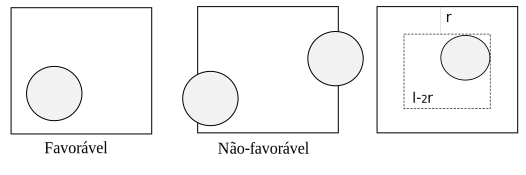
\includegraphics[angle=0, scale=0.5]{fig7.pdf}
\end{center}
\caption{\label{fig7} Representação esquemática do jogo dos ladrilhos.
}
\end{figure} 
Portanto, a probabilidade da moeda cair inteiramente
dentro de um ladrilho é $$ \frac{( l-2r )^2}{l^2}.$$
Se consideramos um piso formado por quadrados de cerâmica de 30 cm de lado e um disco (``moeda'') de raio 5 cm, a probabilidade do disco cair inteiramente dentro de um dos ladrilhos é igual a $(30-10)^2/ 30^2 = 0,4444$ ou 44,44\%.


Nessa situação, o diâmetro $d$ do disco que daria 60\% de chances de vitória ao jogador é $d$ = 6,77 cm.
\end{frame}
%=====================================================================

%=====================================================================
\begin{frame}{Propriedades da probabilidade}
Seja $(\Omega, {\cal F}, P)$ um espaço de probabilidade então $P$ satisfaz as seguintes propriedades:

\begin{enumerate}
\item[P.0] $P(\emptyset)=0.$ De fato, $1=P(\Omega)=P(\Omega \cup \emptyset \cup \emptyset\cup \emptyset\cup \emptyset \cdots )$ $=P(\Omega)+P(\emptyset)+P(\emptyset)+P(\emptyset)+\cdots,$  se e somente se,  $0 \leq P(\emptyset)\leq 1$ caso contrário contradiz [K.2].

\item[P.1] Seja $A$ um evento de ${\cal F}$  e $A^\complement$ o evento complementar, então $$P(A) = 1 - P\left(A^\complement\right).$$ 
De fato, sendo $ \Omega $ o espaço amostral, temos que $\Omega=A\cup A^\complement$ onde a união é disjunta, uma vez que $ A\cap A^\complement=\emptyset $. Utilizando [K.3]  segue que
$$P(\Omega)=P(A)+P\left(A^\complement\right)\Rightarrow P\left(A^\complement\right)=P(\Omega)-P(A)=1-P(A).$$ 


\item[P.2] A probabilidade de ocorrência de eventos associados a um experimento pode ser calculada através da regra da soma da probabilidade para a união de dois eventos. 
Sejam $A$ e $B$  dois eventos em  ${\cal F}$ a probabilidade da união destes dois eventos  é dada por $$ P(A\cup B) = P(A)+P(B)-P(A\cap B).$$ 
De fato, se $ A\cup B=A\cup (B- A) $ e $ A\cap(B - A)=\emptyset $, então $P(A\cup B)=P(A)+P(B - A).$ Agora para $ B=(B- A)\cup(A\cap B) $ com $ (B - A)\cap(A\cap B)=\emptyset $, então
$P(B)=P(B -s A)+P(A\cap B).$ Combinando estes dois resultados, temos que \[P(A\cup B)=P(A)+P(B)-P(A\cap B).\]
\end{enumerate}
\end{frame}
%=====================================================================

%=====================================================================
\begin{frame}
\begin{enumerate}
\item[P.3]  Sejam $A$, $B$ e $C$ três eventos em ${\cal F}$, então 
$$
\begin{aligned}
P(A\cup B\cup C) & = P(A)+P(B)+P(C)-P(A\cap P) \\ &-B(A\cap C)-P(B\cap C)+P(A\cap B\cap C).
\end{aligned}
$$ 
De fato, temos que $A\cup B\cup C=(A\cup B)\cup C=(A\cup B)\cup (C - (A\cup B))$ por ser esta união disjunta. Então por [K.3], temos 
\begin{equation}
\label{eqp1}
P(A\cup B\cup C)=P(A\cup B)+P(C - (A\cup B)) 
\end{equation} 
e utilizando a equação \eqref{eqp1} temos 
$P(A\cup B\cup C)=P(A)+P(B)-P(A\cap B)+P(C - (A\cup B)).$ Mas, $$ C=(C - (A\cup B))\cup(C\cap(A\cup B)),$$ portanto \begin{equation}
\label{eqp2}
P(C - (A\cup B))=P(C)-P(C\cap(A\cup B)).
\end{equation}	
Além disso, temos que $ C\cap (A\cup B)=(C\cap A)\cup (C\cap(B -  A)) $, e esta união é disjunta. Logo,  
\begin{equation}
\label{eqp3}
P(C\cap (A\cup B))=P(A\cup C)+P(C\cap(B - A)).
\end{equation} 	
Finalmente, para $ C\cap B = (A\cap B\cap C)\cup (C\cap(B - A)) $, o que implica que 
\begin{equation}
\label{eqp4}
P(C\cap(B - A))=P(B\cap C) - P(A\cap B\cap C),
\end{equation} 		
já que a união é disjunta. 
\end{enumerate}
\end{frame}
%=====================================================================

%=====================================================================
\begin{frame}


\begin{enumerate}
\item[]	Combinando as equações \eqref{eqp1}, \eqref{eqp2}, \eqref{eqp3} e \eqref{eqp4}, concluímos que 
	\[
	\begin{aligned}
	P(A\cup B\cup C)&=P(A)+P(B)+P(C) - P(A\cap B) \\ & - P(A\cap C)  - P(B\cap C)  +P(A\cap B\cap C).
	\end{aligned}
	\]
\item[P.4] Sejam  $A$ e $B$ eventos de ${\cal F}$ com $A  \subset  B$, então $P(A) \leq P(B).$ De fato, temos que se $ A\subset B $ então $ B = A\cup (B - A) $ e  $ \emptyset = A\cap (B - A) .$  Portanto, utilizando [K.3] segue que 
\[P(B)=P(A)+P(B- A).\] 	 
Como $ P(B - A)\geq 0 $, temos então que $ P(B)\geq P(A).$

\item[P.5] Se $ A\subset B$ então  $$P(B- A)=P(B)-P(A).$$ De fato, note que $ B=A\cup (B- A) $, e ainda que $ A\cap (B - A)=\emptyset $. Assim, ao usarmos [K.3] temos $P(B)=P(A\cup (B- A))=P(A)+P(B- A),$ o que implica $$P(B- A)=P(B)-P(A).$$ 	
\end{enumerate}
\end{frame}



%%=====================================================================
%\begin{frame}{Propriedades de continuidade da probabilidade}
%\begin{enumerate}
%
%\item[P.6] Sejam $ A_1,A_2, \cdots $ eventos aleatórios de ${\cal F}$ tais que $ A_n \downarrow \emptyset $, ou seja, $ A_1 \supseteq A_2 \supseteq \cdots $ e ainda o $ \displaystyle \lim_{n\rightarrow \infty}A_n=\emptyset $, então $ P(A_n)\rightarrow 0.$ 
%$$A_1=(A_1- A_2)\cup (A_2 - A_3)\cup \cdots =  \bigcup_{i=1}^{\infty}(A_i- A_{i+1})$$ 	e  para cada $i$, $ A_i-  A_{i+1} $ são conjuntos disjuntos, pois a sequência é uma sequência decrescente. Por [A.3] temos  que $$P(A_1)=P\left(\bigcup_{i=1}^{\infty}(A_i- A_{i+1})\right)=e\sum_{i=1}^{\infty}P(A_i - A_{i+1}).$$ Por [P.5] temos que $ P(A_i- A_{i+1})=P(A_i)-P(A_{i+1}) $, e portanto 
%$$P(A_1)=\displaystyle \lim_{n \rightarrow \infty} \displaystyle\sum _{i=1}^{n-1}P(A_i-  A_{i+1}).$$ 	Os termos do somatório vão se cancelando restando apenas o primeiro e o último, assim 
%$$
%\begin{aligned}
%P(A_1) & = \displaystyle \lim_{n \rightarrow \infty} P(A_1) - P(A_n)  \\ &=P(A_1) - \lim_{n \rightarrow \infty} P(A_n) \Rightarrow \lim_{n \rightarrow \infty}P(A_n)=0.
%\end{aligned}
%$$ 	 
%Logo  $ P(A_n)\rightarrow 0 $.
%\end{enumerate}
%\end{frame}
%%=====================================================================

%=====================================================================
\begin{frame}


\begin{enumerate}
\item[P.6] No caso geral em que $ A_n \downarrow A $ temos que $(A_n - A) \downarrow \emptyset,$ então, $ P(A_n - A)\rightarrow 0.$  Uma vez que $A \subseteq A_n,$ temos  $P(A_n - A)= P(A_n) - P(A)\rightarrow 0,$ ou seja $ \lim_{n \rightarrow \infty}P(A_n)=P(A).$
	
\item[P.7]   (\textcolor{blue}{Desigualdade de Boole}) Sejam $ A_1, A_2, \cdots , A_n $ uma sequência de eventos aleatórios, então $$ P\left(\bigcup_{i=1}^{n}A_i\right)\leq \sum_{i=1}^{n} P(A_i).$$ Para mostrar esta propriedade vamos usar indução finita. Inicialmente mostremos que $ P(A_1\cup A_2)\leq P(A_1)+P(A_2).$ De fato pela propriedade P.2 
$$
\begin{aligned}
P(A_1\cup A_2)&=P(A_1)+P(A_2)-P(A_1\cap A_2)  \Rightarrow P(A_1\cup A_2)\leq P(A_1)+P(A_2),
\end{aligned}
$$ 
já que $ P(A_1 \cap A_2)\geq 0 $.  Agora vamos supor que esta propriedade seja válida para $n-1$, ou seja, que $ P\left(\displaystyle \bigcup_{i=1}^{n-1}A_i\right)\leq \displaystyle\sum_{i=1}^{n-1} P(A_i) $ e mostremos que é válida para $n.$ $$
\begin{aligned}
P\left(\bigcup_{i=1}^{n}A_i\right)& =P\left(\bigcup_{i=1}^{n-1}A_i \cup A_n\right) =P(C \cup A_n)=P(C)+P(A_n)-P(C\cap A_n) \\ & \leq P(C)+P(A_n),
\end{aligned}
$$ em que $ C= \bigcup_{i=1}^{n-1}A_i $, e ao usarmos a hipótese de indução temos que 
$$ P(C)+P(A_n)\leq \sum_{i=1}^{n-1} P(A_i) + P(A_n)= \sum_{i=1}^{n} P(A_i).$$ 
\end{enumerate}

\end{frame}
%=====================================================================

\begin{frame}
	
	
	\begin{corol} Para $n$ eventos arbitrários $\{A_1,\ldots,A_n\}$,
	$$P(\inter A_i)\geq \sum_{i=1}^{n}P(A_i)-(n-1).$$ \end{corol}
	
	\begin{proof} Utilizando a Lei de De Morgan e a desigualdade de Boole para os
	eventos $\{A_1^c,\ldots,A_n^c\}$, temos
	$$P(\union_{i=1}^{n}A_i^c)=1-P(\inter A_i)\leq \sum_{i=1}^{n}P(A_i^c)=\sum_{i=1}^{n}(1-P(A_i)).$$
	Logo,
	$$P(\inter A_i)\geq \sum_{i=1}^{n}P(A_i)-(n-1).$$ \end{proof}
\end{frame}

%=====================================================================
\begin{frame}
\begin{enumerate}
\item[P.8]  Sejam $ A_1, A_2, \cdots $ eventos de ${\cal F}$, então $ P\left( \bigcup_{i=1}^{\infty}A_i\right)\leq \sum_{i=1}^{\infty} P(A_i).$ 

De fato,  se definimos $ C_n=\displaystyle \bigcup_{i=1}^{n}A_i $, temos que $ C_n\uparrow C $, no qual $C$ é definido como $ C= \bigcup_{i=1}^{\infty}A_i $. Por continuidade sabemos que $ P(C_n)\uparrow P(C) $. Usando a propriedade P.7 temos que $$ P(C_n)= P\left(\displaystyle \bigcup_{i=1}^{n}A_i\right)\leq  \sum_{i=1}^{n} P(A_i),$$ por outro lado 
$$
\begin{aligned}
P\left( \bigcup_{i=1}^{\infty}A_i\right)= P(C)=\lim_{n\rightarrow \infty}P(C_n)  \leq\lim_{n\rightarrow \infty}\sum_{i=1}^{n} P(A_i)= \sum_{i=1}^{\infty} P(A_i),
\end{aligned}$$ 
% ou seja $ P\left( \bigcup_{i=1}^{\infty}A_i\right)\leq \sum_{i=1}^{\infty} P(A_i) $.


%\item[P.9]  $ P\left(\displaystyle \bigcap_{k=1}^{n} A_k\right)\geq 1- \displaystyle\sum_{k=1}^{n} P\left(A_{k}^\complement\right) $. 
%
%De fato, pelas leis de De Morgan temos que 
%$ \displaystyle \bigcup_{k=1}^{n}A_k^\complement=\left(\displaystyle\bigcap_{k=1}^{n}A_k\right)^\complement $. Assim, usando P.8 
%$$1-P\left(\displaystyle\bigcap_{k=1}^{n}A_k\right) = P\left[\left(\displaystyle\bigcap_{k=1}^{n}A_k\right)^\complement\right] = P\left(\bigcup_{k=1}^{n}A_k^\complement\right)$$
%$$\Rightarrow P\left(\displaystyle \bigcap_{k=1}^{n} A_k\right)\geq 1- \displaystyle\sum_{k=1}^{n} P\left(A_{k}^\complement\right).$$ 	
\end{enumerate}
\end{frame}
%=====================================================================

%=====================================================================
\begin{frame}{Princípio da Inclusão-Exclusão:} O princípio da inclusão-exclusão permite determinar o cardinal da união de vários conjuntos tomando como base os cardinais da cada um deles e todas as suas possíveis interseções. 
Sejam  $A_1,\ldots, A_n$  conjuntos finitos,  então:
$$
\begin{aligned} 
\biggl|\bigcup_{i=1}^n A_i\biggr| & =\sum_{i=1}^n\left|A_i\right| - \sum_{i,j\,:\,1 \le i < j \le n}\left|A_i\cap A_j\right| \\ &+\sum_{i,j,k\,:\,1 \le i < j < k \le n}\left|A_i\cap A_j\cap A_k\right| \\
& -\ \cdots\ + \left(-1\right)^{n-1} \left|A_1\cap\cdots\cap A_n\right|. 
\end{aligned}
$$

Para o caso de dois conjuntos $A$ e $B$ finitos temos $|(A - B) \cup (B - A) \cup (A\cap B) = |(A - B)| + |(B - A)|+|(A\cap B)$  por serem disjuntos. 

Por outro lado $|(A - B)|=|A|+|A \cap B|$ e $|(B - A)|=|B|+|A \cap B|.$ 

Juntando essa duas expressões temos que 
$|A \cup B| = |A|-|A \cap B| + |B|-|A\cap B| + |A\cap B|,$ logo $$|A \cup B| = |A|-|B|-|A\cap B|.$$

\end{frame}
%=====================================================================

%=====================================================================
\begin{frame}
Como uma exemplificação verifiquemos a fórmula para o caso de termos três conjuntos $A,$ $B$ e $C$ finitos.  Para isto, observemos o diagrama de Venn-Euler (Figura \ref{fig3}) que representa o conjunto $(A \cup B \cup C)$ o qual permitirá construir o argumento para verificar o princípio de inclusão-exclusão para o caso $n=3.$

\begin{figure}[!htb]
\begin{center}
\includegraphics[angle=0, scale=0.22]{fig3.pdf}
\caption{\label{fig3}  Representação gráfica do conjunto $(A \cup B \cup C)$ para a verificação do princípio de inclusão-exclusão.}
\end{center}
\end{figure} 
Assim, 
$$
\begin{aligned}
|A \cup B \cup C| &= |A \cup (B \cup C)| \\
&= |A| + |B \cup C| - |A \cap (B \cup C)| \\
&= |A| + |B| + |C| - |B \cap C| - |(A \cap B) \cup (A \cap C)| \\
&= |A| + |B| + |C| - |B \cap C| - (|A \cap B| + |A \cap C| - |A \cap B \cap C|) \\
&= |A| + |B| + |C| - |A \cap B| - |A \cap C| - |B \cap C| + |A\cap  B \cap C|. \\
\end{aligned}
$$
O qual verifica a fórmula para $n=3.$
\end{frame}
%=====================================================================

%=====================================================================
\begin{frame}
\begin{exem}
Quantos são os números inteiros positivos menores que 504 e primos com 504? 
Usando a decomposição em fatores primos temos que $504 = 2^3 \times 3^2 \times 7.$ Agora, definimos os conjuntos 

$$
\begin{aligned}
A & = \{1, 2, \ldots , 504\},\\
A_1 &= \{x \in A : x \ \text{é múltiplo de} \ 2\},\\
A_2 &= \{x \in A : x \ \text{é múltiplo de} \ 3\}, \\
A_3 &= \{x \in A : x \ \text{é múltiplo de} \ 7\}. \\
\end{aligned}
$$
Desejamos calcular a cardinalidade do conjunto $A - (A_1 \cup A_2 \cup A_3 )$. Desta forma, 
$|A_1|= 504/2 = 252,$
$|A_2|= 504/3 = 168,$ 
$|A_3|= 504/7 = 72,$ 
$|A_1 \cap A_2 | = 504/ (2\times 3) = 84,$ 
$|A_1 \cap A_3| = 504/  (2\times 7) = 36,$ 
$|A_2 \cap A_3 | = 504/ (3\times 7)=  24,$  
$|A_1 \cap A_2 \cap A_3 | = 504/ (2\times 3\times 7)=  12. $ 
Usando o princípio de inclusão-exclusão
$$|A_1 \cup A_2 \cup A_3 | = 252 + 168 + 72 - 84 - 36 - 24 + 12 = 360.$$
Assim, existem ao todo 144 números inteiros positivos menores que 504 e primos com 504.
\end{exem}
\end{frame}
%=====================================================================



\begin{frame}{Princípio da Inclusão-Exclusão para probabilidade}
	
	O próximo teorema permite que possamos calcular de maneira exata a
	probabilidade $P(\union_{i=1}^{n}A_i)$ para $n$ eventos arbitrários.
	
	\begin{teo} {\bf Princípio da Inclusão-Exclusão.}  Seja $I$ um conjunto
	genérico de índices que é um subconjunto não-vazio qualquer de
	$\{1,2,\ldots,n\}$. Para eventos arbitrários $\{A_1,\ldots,A_n\}$,
	$$P(\union_{i=1}^{n}A_i)=\sum_{\emptyset\ne I\subseteq \{1,\ldots, n\}}(-1)^{|I|+1}P(\inter_{i\in I}A_i),$$
	onde o somatório é sobre todos os $2^n-1$ conjuntos de índices
	excluindo apenas o conjunto vazio. \end{teo}
	
	No caso particular de $n=3$, o princípio de inclusão-exclusão afirma
	que
	\begin{eqnarray}
	& & P(A_1\union A_2\union A_3)=P(A_1)+P(A_2)+P(A_3)\nonumber\\
	& & -P(A_1\inter A_2)-P(A_1\inter A_3)-P(A_2\inter A_3)\nonumber\\
	& & +P(A_1\inter A_2\inter A_3).\nonumber
	\end{eqnarray}
	
\end{frame}

\begin{frame}
\begin{proof} A prova é por indução matemática em $n$. O resultado é
trivialmente verdadeiro para $n=1$ e já foi provado para $n=2$ na propriedade P.2. Assuma que o resultado vale para $n=k$ e
vamos provar que ele é verdadeiro para $n=k+1$. Como na prova da
desigualdade de Boole, $\union_{i=1}^{k+1}A_i=A_{k+1}\union
(\union_{i=1}^{k}A_i)$. Usando o resultado para $n=2$, temos
$$P(\union_{i=1}^{k+1}A_i)=P(A_{k+1})+P(\union_{i=1}^{k}A_i)-P(A_{k+1}\inter (\union_{i=1}^{k}A_1)).$$
Reescrevendo o último termo como $P(\union_{i=1}^{k}(A_{k+1}\inter
A_i))$, nos dá uma expressão que contém uma união de exatamente $k$
conjuntos. Então, usando a hipótese do passo indutivo para os dois
últimos termos
\begin{eqnarray}
& & P(\union_{i=1}^{k+1}A_i)=P(A_{k+1})+\sum_{\emptyset\ne I\subseteq\{1,\ldots,k\}}(-1)^{|I|+1}P(\inter_{i\in I}A_i)\nonumber\\
& & -\sum_{\emptyset\ne I\subseteq\{1,\ldots,k\}}(-1)^{|I|+1}P(\inter_{i\in I}(A_{k+1}\inter A_i)).
\nonumber\end{eqnarray}
O resultado segue ao rearranjarmos os termos destes somatórios.
\end{proof}
\end{frame}





%=====================================================================
\begin{frame}{Variações com repetição: Amostras com ordem e com substituição.} Suponhamos que temos uma gaveta com $n$  objetos distintos. Desejamos realizar $k$ extrações ao acaso de um objeto ao mesmo tempo. Ao efetuar uma extração, registramos o objeto escolhido (marcamos o objeto, isto é o distinguimos) e o devolvemos à gaveta, desta forma o objeto pode ser selecionado várias vezes. Em cada extração temos $n$ objetos possíveis para serem escolhidos e efetuamos $k$ extrações. 

Assim pelo princípio da multiplicação o número total de arranjos que podem ser obtidos desta gaveta ao se fazer $k$ extrações é 
$$\displaystyle{\underbrace{n\cdot n\cdots n}_{\text{\normalsize $n$ vezes}}=n^k.}$$ 
Este número é chamado de {\it ordenações com repetição}. 

\begin{exem}
Suponhamos que temos um conjunto de 60 caracteres distintos. este conjunto contém todas as letras minúsculas e as letras maiúsculas do alfabeto, os dez dígitos e alguns caracteres especias como: $\%, @, \$, \#,$ etc. Quantas senhas de comprimento 6 podem ser construídas usando estes 60 caracteres?

Como cada caracter dos 60 disponíveis pode ser escolhido para ser colocado em cada uma das seis posições da senha, então podemos construir $60 \times 60 \times 60 \times 60 \times 60 \times 60= 60^6 =4.6656\times 10^{10} $ distintas senhas.
\end{exem}


\end{frame}
%=====================================================================

\begin{frame}
\vspace{4cm}
\begin{block}{Extra: Técnicas para contagem }
	{}
\end{block}
\end{frame}
%=====================================================================
\begin{frame}{Variações sem repetição: Amostras com ordem e sem substituição.} Temos uma gaveta com $n$ objetos e dos quais se devem extrair, um a um $k$ objetos. Suponhamos que nesta situação a amostra é {\it sem substituição}, isto quer dizer, uma vez selecionado um  objeto este não é devolvido à gaveta. O total de arranjos distintos que podemos obter é 
\begin{equation}
\label{perm1}
n(n-1)(n-2)\cdots (n-k-1). 
\end{equation}
Pelo princípio da multiplicação notamos que há $k$ fatores na expressão anterior. O primeiro fator é $n$ e isto é devido ao fato que temos qualquer dos $n$ objetos para serem colocados na primeira posição, para a segunda posição temos $(n-1)$ objetos, para a terceira posição $(n-2)$ objetos, e assim por diante. este raciocínio termina ao escolher o $k$-ésimo objeto para o qual temos unicamente $(n-k+1)$ possibilidades. A expressão anterior pode ser escrita como 
$$
P(n,k) = \frac{n!}{(n-k)!}, \quad k \leq n
$$ 
e se chama de {\it permutação de $n$ em $k$}. 
\begin{exem}
De quantas formas podem ser atribuídos ou primeiro, segundo e terceiro prêmio em uma rifa de 10 boletos numerados de 1 até 10? Notemos que de fato este problema é um problema de ordenação sem repetição de 10 objetos em que devem ser extraídos 3 objetos de estes. Daí, existem $10\times 9\times 8=720 $ distintas atribuições para os três primeiros números na rifa. 
\end{exem}


\end{frame}
%=====================================================================


%=====================================================================
\begin{frame}{Permutações: Amostras exaustivas com ordem e sem substituição.} A pergunta básica a respeito do número total de formas em que podemos colocar em um ordem linear (um  elemento após o outro e portanto sem repetição) $n$ objetos distintos tem com resposta o chamado {\it fatorial} de| $n,$ o qual é denotado por $$n! = n(n-1)(n-2)\cdots 3\cdot 2 \cdot 1.$$ Por definição temos que $0!=1.$

\begin{exem}
Suponhamos que queremos acomodar algumas crianças em uma fila, quatro meninas e três meninos. Se os meninos e meninas podem ser alocados em qualquer ordem então há $7!=5040$ formas de acomodar as crianças. Agora se queremos que os meninos e as meninas fiquem alternados na fila então há 
$(4\times 3) \times (3\times 2) \times (2\times 1) \times 1 = 144$ formas de organizá-los. Se desejamos que os meninos formem um grupo e as meninas formem outro grupo na fila temos $2\times 4! \times 3! =288$ formas de acomodá-los. 
\end{exem}

\end{frame}
%=====================================================================


%=====================================================================
\begin{frame}{Combinações: Amostras sem ordem e sem substituição} Suponhamos  que temos um conjunto de $n$ objetos distinguíveis e estamos interessados em obter uma amostra (subconjunto)  de tamanho $k.$ Suponhamos que as amostras agora devem ser {\it sem ordem e sem repetição}.  Lembremos que quando a ordem importa temos ${n!}/{(n-k)!}$ possibilidades. Agora, como não estamos interessados na ordem observamos que um dos arranjos desta fórmula está sendo contado $k!$ vezes. As vezes em que os mesmos $k$ elementos podem ser permutados uns com os outros, uma vez que o conjunto de dados é o mesmo. Assim, para obter arranjos em que a ordem não importa devemos então dividir por $k!.$ Está fórmula se chama de {\it combinações de $n$ em $k$} a qual é denotada por 
\begin{equation}
\label{comb}
C_n^k = {n\choose k} = \frac{n!}{k!\cdot\left(n - k\right)!}, 
\end{equation}
em que  $n$ é o total de elementos e $k$ é o número de elementos escolhidos. 

Note que da equação \ref{comb} pode ser deduzido que 
\begin{equation}
\label{comb2}
{n \choose k} = {n \choose n-k} .
\end{equation}
De fato, se o número $\displaystyle{{n \choose k}}$ representa o número de subconjuntos de $k$ elementos
de um conjunto de $n$ elementos, então, se inicialmente escolhemos $k$ objetos estamos deixando de lado $n-k$ objetos, que é equivalente a escolher $n-k$ objetos que logo serão deixados de lado.

\end{frame}
%=====================================================================

%=====================================================================
\begin{frame}
\begin{exem}{Megassena}
Uma importante aplicação de combinação  é nas loterias:
Megassena, quina entre outras. A megassena consiste em uma cartela de 60
números dentre os quais devemos acertar 6 (prêmio principal). Calcule a
quantidade total de resultados possíveis para o prêmio principal.

Para marcar um cartão, precisamos escolher 6 entre 60 números, em que a
ordem de escolha não interfere no cartão que será marcado. Trata-se portanto, de
acordo com a definição, de um problema de combinação (devemos
combinar 60 números, em grupos de 6 números, ou seja, queremos subconjuntos
de 6 elementos de um conjunto de 10 elementos). O número de cartões é 
$$\displaystyle
{60 \choose 6} = 50063860
$$

\end{exem}

\begin{exem}
Seja $A$ um conjunto finito com $n$ elementos, então $A$ possui $2^n$ subconjuntos. De fato, sabemos que o coeficiente  
$\displaystyle{{n \choose k}}$ representa o número de subconjuntos de $k$ elementos de um conjunto de $n$ elementos. 
Então, se somamos em $k$ ($k=0$ elementos, $k=1$ elementos, e assim por diante ate $k=n$ elementos ) obtemos o número de subconjuntos do conjunto $A$. 
$$
{n \choose 0} + {n \choose 1} + {n \choose 2} + \cdots + {n \choose n} = (1+1)^n = 2^n.
$$
\end{exem}

\end{frame}
%=====================================================================



\begin{frame}
\vspace{4cm}
\begin{block}{Extra: Exercícios - Exemplos }
	{}
\end{block}
\end{frame}


\begin{frame}
\begin{exem}{Modelos de gavetas} Suponhamos que em uma caixa há $N$ bolas do mesmo tipo, mas de cores diferentes, a saber: $R$ bolas
vermelhas e $N-R$ brancas. Se extraem ao  acaso $n$ bolas. Qual é  a probabilidade de extrair exatamente $k \leq n$ bolas vermelhas?
\end{exem}

\begin{block}{Caso I}
Suponhamos que as bolas se encontram  enumeradas de 1 até $N$ e que a enumeração das bolas vermelhas vá de 1 até $R$. Nesta situação devemos lembrar que é necessário distinguir dois casos. A extração é feita com substituição  e a  extração é feita sem substituição. No primeiro caso podemos considerar duas alternativas: 

\begin{enumerate}
\item[i)] As bolas são retiradas uma após a outra : As $n$ bolas são extraídas uma a uma da caixa e deixadas fora da caixa. Neste caso o espaço 
amostral está dado por:
$$\Omega= \{ (a_1, a_2, \dots \, , a_n): a_j \in \{1,2,\dots \, , N \} \, , a_i \not= a_j, i \not= j, j=1,2, \dots , n \}$$  
Então, definimos os eventos 
\begin{center}
$A_k$=``exatamente $k \leq n$ bolas vermelhas são extraídas''.
\end{center}
Note que $A_k$ é uma $n$-upla em $\Omega ,$ que contém exatamente $k$ componentes menores ou iguais a $R$. Temos desta forma que: 



\end{enumerate}
\end{block}
\end{frame}
%=====================================================================


%=====================================================================
\begin{frame}
\begin{block}{}
	\begin{equation*}\displaystyle
	\begin{aligned}
	\left| \Omega \right| &=  N(N-1)...(N-(n-1))=(N)_n \\
	\left| A_k \right| &= \binom{n}{k} R(R-1) ... (R-k+1)(N-R)...(N-R-(n-k)+1) \\
	&=\binom{n}{k}P(R,k) P(N-R, n-k). \\
	\end{aligned}
	\end{equation*}
	
Agora, ao supormos que o experimento é Laplaciano, tem-se
\begin{equation*}
P(A_k)=\frac{\left|A_k \right|}{ \left|\Omega\right|}= \displaystyle{\frac{\binom{R}{k} \binom{N-R}{n-k} }{ \binom{N}{n}}} .
\end{equation*}
\begin{enumerate}
\item[ii)] As bolas são todas retiradas ao mesmo tempo: As $n$ bolas são todas extraídas ao tempo; neste caso temos que 
$\Omega =\{T:T \subseteq\{1,2,\ldots,N \}, \text{com}  \left|T\right|=n\}$ e $A_k$ definido como em i) consta de
todos os subconjuntos de  $\{1,2,  \dots ,N\}$ que contém  exatamente $k$ componentes menores ou iguais a $R$. Desta
forma  $\left| \Omega\right|= \binom{N}{n} $  e $\left| A_k\right|= \binom{R}{k} \binom{N-R}{n-k}.$ Ao supor novamente que o experimento é Laplaciano 
\begin{equation*} 
\displaystyle{P(A_k)=\frac{\binom{R}{k} \binom{N-R}{n-k} } { \binom{N}{n}}}.
\end{equation*}

%Se unicamente interessa o número $k$ de bolas vermelhas entre as $n$
%bolas extraídas da caixa, temos que
%\begin{equation*} 
%\displaystyle{p_k= \frac{\binom{R}{k} \binom{N-R}{n-k}}{
%\binom{N}{n}}  , \quad k = 0,1,2, \dots , n}
%\end{equation*} 
Aqui, $p_k=P(A_k)$ define uma medida de probabilidade sobre o conjunto $\Omega^\prime=\{0,1, \dots  , n\} $, chamada de \textit{distribuição
hipergeométrica} com parâmetros $n$, $R$ e $N$, a qual é denotada por $H_g (n,R,N)$. 
\end{enumerate}
\end{block}
\end{frame}
%=====================================================================

%=====================================================================
\begin{frame}
\begin{block}{Caso II}
No segundo caso, a extração é com substituição, cada bola extraída  é devolvida imediatamente à caixa; depois de misturar as bolas, extrai-se aleatoriamente a seguinte bola e  assim por diante. Neste caso, temos que o espaço amostral é igual a: 
$$
\begin{aligned}
\Omega &= \{(a_1, a_2, \ldots \, , a_n) : a_j \in \{1,2, \dots , N\},\ j= 1,2, \dots , n\}\\
&=\{1,\dots , N\}\times \{1, \dots , N\}\times \cdots \times\{1, \dots , N\} =\{1, \dots , N\}^n,  
\end{aligned}
$$
e o evento $A_k$ consta de todos os elementos $ (a_1, a_2, \ldots \, , a_n) \in \Omega$ com exatamente 
$k$ componentes menores ou iguais a $R$. Temos assim, $ \left| \Omega \right| =  N\cdot N \, \cdots \, N=N^n$ e $$\left|A_k \right|=\binom{n}{k}R^k(N-R)^{n-k}. $$ Portanto, se supursemos que todas as bolas têm a mesma chance de serem extraídas, então 
$$p_k=P(A_k)=\binom{n}{k}\frac{R^k(N-R)^{n-k}}{N^n}=\binom{n}{k}p^k q^{n-k},$$ em que $p=R/N$ e $q=1-p.$ 
Se estamos interessados unicamente no número $k$ de bolas vermelhas entre as $n$ bolas extraídas,  temos que

$$p_k= \binom{n}{k}p^k q^{n-k}, \qquad k=0,1,2,\dots , n, \qquad 0<p<1, q=1-p$$ define una medida de probabilidade sobre o conjunto 
$\Omega^\prime =\{0,1,2, \dots ,n\}$  chamada de  \textit{distribuição binomial} com parâmetros $n$ e $p$ a qual é denotada por ${\cal B}(n,p).$ 
\end{block}
\end{frame}
%=====================================================================



\begin{frame}
\vspace{-0.3cm}
\begin{exer}
		Se $A$, $B$ e $C$ forem eventos mutuamente excludentes, com $P(A)=0{,}2$, $P(B)=0{,}3$ e $P(C)=0{,}4$, determine:
		\begin{enumerate}
			\item[(a)] $P(A\inter B\inter C)$.
			\item[(b)] $P(A^c\union(B\union C))$.
			\item[(c)] $P((A\union B)\inter C)$.
		\end{enumerate}
		
	\end{exer}
	
	\begin{exer}
		Se $A$, $B$ e $C$ forem eventos mutuamente excludentes, será possível obter $P(A)=0{,}3$, $P(B)=0{,}4$ e $P(C)=0{,}5$? Justifique.
	\end{exer}

\begin{exer}
Se $\Omega=\{a,b,c\}$, e a álgebra $\A$ é o conjunto das partes de
$\Omega$, e a medida de probabilidade $P$ é parcialmente definida
por
$$P(\{a,b\})=0.5\mbox{,  }P(\{b,c\})=0.8\mbox{,  }P(\{a,c\})=0.7,$$
então complete a especificação de $P$ para todos os eventos em $\A$.
\end{exer}

\begin{exer}
Se $\{A_i\}$ for uma partição enumerável de $\Omega$ e
$P(A_i)=ab^i$, $i\geq 1$, então quais as condições que $a$ e $b$
devem satisfazer para que $P$ seja uma medida de probabilidade?
\end{exer}

%\end{block}
\end{frame}

\begin{frame}

\begin{exem}
Em um grupo de $r$ pessoas qual a probabilidade de haver pelo menos
duas pessoas que façam aniversário no mesmo dia, assumindo que a
distribuição de aniversários é uniforme ao longo do ano e
desprezando a existência de anos bissextos?
\end{exem}

{\bf Solução:} O número de resultados possíveis para os
aniversários de $r$ pessoas é $365^r$. O número de casos possíveis
onde todas as pessoas fazem aniversário em dias diferentes é dado
por $365\times 364\times \cdots\times(365-(r-1))$. Portanto, o
número de casos possíveis onde pelo menos duas pessoas fazem
aniversário no mesmo dia é a diferença entre o número total de
aniversários possíveis e o número de casos onde as pessoas têm
aniversários em datas diferentes, ou seja, é igual a
$$365^r-365\times 364\times \cdots\times(365-(r-1)).$$
Logo, a probabilidade deste evento é:
$$1-\frac{365\times 364\times \cdots\times(365-(r-1))}{365^r}.$$
Para $r=23$, temos que essa probabilidade é aproximadamente igual a
$0,51$. E para $r=50$, essa probabilidade é igual a $0,97$.

%\end{block}
\end{frame}

\begin{frame}
\begin{exem}
Em uma loteria de $N$ números há um só prêmio. Salvador compra $n$
$(1<n<N)$ bilhetes para uma só extração e Sílvio compra $n$
bilhetes, um para cada uma de $n$ extrações. Qual dos dois jogadores
têm mais chances de ganhar algum prêmio?
\end{exem}

{\bf Solução:} A probabilidade de Salvador ganhar algum prêmio é
$\frac{n}{N}$. O número total de $n$ extrações possíveis é $N^n$. O
número de casos onde Sílvio não ganha nenhum prêmio é $(N-1)^n$,
logo o número de casos onde Sílvio ganha algum prêmio é igual a
$N^n-(N-1)^n$. Logo, a probabilidade de Sílvio ganhar algum prêmio é
$1-\frac{(N-1)^n}{N^n}$.

Vamos provar por indução que Salvador tem mais chance de ganhar, ou
seja, $\frac{n}{N}>1-\frac{(N-1)^n}{N^n}$, que equivale a
$$\frac{(N-1)^n}{N^n}>1-\frac{n}{N}.$$
Para $n=2$, temos:
$$\frac{(N-1)^2}{N^2}=1-\frac{2}{N}+\frac{1}{N^2}>1-\frac{2}{N}.$$
\end{frame}

\begin{frame}

{\bf Solução (cont.)} Suponha que para $n=k$, temos que
$$\frac{(N-1)^k}{N^k}>1-\frac{k}{N}.$$
Multiplicando esta expressão por $\frac{N-1}{N}$, obtemos:
\begin{eqnarray}
& & \frac{(N-1)^{k+1}}{N^{k+1}}>(\frac{N-1}{N})(1-\frac{k}{N})\nonumber\\
& & =1-\frac{1}{N}-\frac{k}{N}+\frac{k}{N^2}>1-\frac{k+1}{N}.\nonumber
\end{eqnarray}


\begin{exem}
Doze pessoas são divididas em três grupos de 4. Qual é a
probabilidade de duas determinadas dessas pessoas ficarem no mesmo
grupo?
\end{exem}

{\bf Solução: } O número total de divisões de doze pessoas em 3
grupos de 4 é igual a $\binom{12}{4}\binom{8}{4}\binom{4}{4}$. Vamos
agora contar o número de casos favoráveis ao nosso evento. Existem 3 opções de escolhermos em qual grupo as duas pessoas determinadas
podem ficar. 
\end{frame}

\begin{frame}
{\bf Solução (cont.)}
Das 10 pessoas restantes, temos que escolher mais duas
para estarem neste grupo, o que podemos fazer de $\binom{10}{2}$
maneiras diferentes. E temos $\binom{8}{4}\binom{4}{4}$ maneiras
diferentes de dividir as outras 8 pessoas nos dois grupos restantes.
Portanto, a probabilidade de duas determinadas pessoas ficarem no
mesmo grupo é:
$$\frac{3\binom{10}{2}\binom{8}{4}\binom{4}{4}}{\binom{12}{4}\binom{8}{4}\binom{4}{4}}=\frac{3}{11}.$$


\begin{exem}
Suponha que temos em uma sala $n$ mães cada uma com um filho. Suponha formemos duplas aleatoriamente, onde cada dupla contém uma mãe e um filho, qual a probabilidade de que pelo menos uma mãe forme uma dupla com seu próprio filho?
\end{exem}

{\bf Solução: } 
Seja $A_i$ o evento que a $i$-ésima mãe forma dupla com seu filho. Queremos determinar
$$P(\cup_{i=1}^{n}A_i).$$
Vamos calcular esta probabilidade utilizando a fórmula da inclusão exclusão. 

\end{frame}

\begin{frame}

{\bf Solução: (cont.)}  Note que:
\begin{eqnarray}
& & P(A_i)=\frac{(n-1)!}{n!}=\frac{1}{n}\mbox{ para todo } i\in\{1,2,\ldots,n\} \nonumber\\
& & P(A_i\cap A_j)=\frac{(n-2)!}{n!}=\frac{1}{n(n-1)}\mbox{ para }i\ne j \nonumber
\end{eqnarray}
e em geral, para um grupo $I\in\{1,2,\ldots,n\}$ de mães temos que
$$P(\cap_{i\in I}A_i)=\frac{(n-|I|)!}{n!}.$$

Como existem $\binom{n}{|I|}$ grupos de mães com cardinalidade $||I||$, temos que
\begin{eqnarray}
& & P(\cup_{i=1}^{n}A_i)=\sum_{i=1}^{n}(-1)^{i+1}\binom{n}{i}\frac{(n-i)!}{n!} \nonumber\\
& & = \sum_{i=1}^{n}(-1)^{i+1}\frac{1}{i!}\nonumber
\end{eqnarray}
Note que quando $n\rightarrow\infty$, temos que esta probabilidade tende a $1-\frac{1}{e}$.
%\end{block}
\end{frame}

\begin{frame}

\begin{exem}
Demonstre que se $P(A_i)=1$ para $i=1,2,\ldots$, então $P(\cap_{i=1}^{\infty}A_i)=1$.
\end{exem}
{\bf Solução: } Como $P(A_i)=1$, temos que $P(A_i^c)=1-P(A_i)=0$. Logo pela não-negatividade e pela desigualdade de Boole, temos
$0\leq P(\cup_{i=1}^{\infty}A_i^c)\leq \sum_{i=1}^{\infty}P(A_i^c)=0$. Portanto, como pela Lei de De'Morgan, $\cap_{i=1}^{\infty}A_i=(\cup_{i=1}^{\infty}A_i^c)^c$, temos que
$P(\cap_{i=1}^{\infty}A_i)=1-P(\cup_{i=1}^{\infty}A_i^c)=1$.


\begin{exem}
Demonstre: se $A_1,A_2,\ldots$ e $B_1,B_2,\ldots$ são eventos aleatórios do mesmo espaço de probabilidade tais que
$P(A_n)\rightarrow 1$ e $P(B_n)\rightarrow p$, então $P(A_n\cap B_n)\rightarrow p$.
\end{exem}

{\bf Solução: } Note que
\begin{eqnarray}
& & P(A_n\cap B_n)=1-P((A_n\cap B_n)^c)=1-P(A_n^c\cup B_n^c) \nonumber \\
& & \geq 1-P(A_n^c)-P(B_n^c)=P(A_n)+P(B_n)-1.
\end{eqnarray}
Como $P(A_n)+P(B_n)-1\rightarrow p$, temos que $\liminf P(A_n\cap B_n)\geq p$. Por outro lado, como $P(A_n\cap B_n)\leq P(B_n)$ e $P(B_n)\rightarrow p$, temos que $\limsup P(A_n\cap B_n)\leq p$. Portanto, $\lim P(A_n\cap B_n)=p$.


%\end{block}
\end{frame}




%
%\begin{frame}
%\frametitle{\textbf{Exemplos de Medida de Probabilidade}}
%\baselineskip=13pt
%%\begin{block}{Exemplos}
%
%\begin{example}
%Se $\Omega$ for um conjunto finito, então temos que a probabilidade
%clássica que assume que todos os resultados são igualmente
%prováveis, é um exemplo de uma medida de probabilidade. Neste caso,
%temos que
%$$P(A)=\frac{||A||}{||\Omega||}$$
%definido para qualquer subconjunto $A$ de $\Omega$. O fato que
%$0\leq ||A||\leq ||\Omega||$ e que
%$$||A\union B||=||A||+||B||-||A\inter B||,$$
%permitem que verifiquemos que $P$ satisfaz os axiomas de Kolmogorov.
%\end{example}
%
%\end{frame}
%
%\begin{frame}
%\frametitle{\textbf{Exemplos de Medida de Probabilidade}}
%\baselineskip=13pt
%
%\begin{example}
%Se $\Omega=\{\omega_1,\omega_2,\ldots,\omega_n\}$ um conjunto
%finito, e seja $P(\{\omega_i\})=p_i$, onde $p_i\geq 0,i\geq 1$ e
%$\sum_{i=1}^{n}p_i=1$, e $P(A)=\sum_{\omega_i\in A}P(\{\omega_i\})$.
%Neste caso, também é fácil verificar que $P$ é uma medida de
%probabilidade verificando os axiomas.
%\end{example}
%
%\begin{example}
%Seja $\Omega=[0,1]$ e $\B_0$ a $\sigma$-álgebra de Borel restrita a eventos contidos em $[0,1]$. Pode-se provar que existe uma medida de probabilidade $\mu$ em $(\Omega,\B_0)$ tal que para todo intervalo $I$ em $[0,1]$ $\mu(I)$ é igual ao comprimento de $I$. Esta medida de probabilidade $\mu$ é conhecida como {\em medida de Lebesgue}.
%\end{example}
%
%%\end{block}
%\end{frame}
%
%\section{Propriedades}
%\begin{frame}
%\frametitle{\textbf{Propriedades de Medida de Probabilidade}}
%\baselineskip=13pt
%\begin{block}{}
%
%\thm Se $P$ é uma medida de probabilidade, então
%\begin{enumerate}
%\item $P(A^c)=1-P(A)$.
%
%\item $P(\emptyset)=0$.
%
%\item $P(A)\leq 1$.
%\end{enumerate}
%\ethm
%\end{block}
%
%\begin{block}{}
%\prv Parte 1, segue do fato que $\Omega=A\union A^c$, K2, e K3, pois
%$$1=P(\Omega)=P(A)+P(A^c).$$
%Parte 2, segue da Parte 1, do fato que $\Omega^c=\emptyset$, e K2,
%K3, pois
%$$P(\emptyset)=1-P(\Omega)=0.$$
%Parte 3, segue do fato que $1=P(\Omega)=P(A)+P(A^c)\geq P(A)$, já
%que $P(A^c)\geq 0$ por K1. \eprv
%
%\end{block}
%\end{frame}
%
%\begin{frame}
%\frametitle{\textbf{Propriedades de Medida de Probabilidade}}
%\baselineskip=13pt
%\begin{block}{}
%
%
%\thm {\bf Monotonicidade.} Se $A\subseteq B$, então $P(A)\leq P(B)$.
%\ethm
%
%\prv Note que $B=A\union(B-A)$, onde $A$ e $B-A$ são disjuntos.
%Então K3 implica que $P(B)=P(A)+P(B-A)$. O resultado segue do fato
%que $P(B-A)\geq 0$. \eprv
%
%\cor $P(A\union B)\geq \max(P(A),P(B))\geq \min(P(A),P(B))\geq
%P(A\inter B)$. \ecor
%
%\end{block}
%\end{frame}
%
%\begin{frame}
%\frametitle{\textbf{Propriedades de Medida de Probabilidade}}
%\baselineskip=13pt
%\begin{block}{}
%
%
%\thm\label{thm:union} Uma expressão exata para a probabilidade de
%uma união não-disjunta é dada por
%$$P(A\union B)=P(A)+P(B)-P(A\inter B).$$
%\ethm
%
%\prv Como $A\union B=A\union (B-A),$ e $A$ e $B-A$ são disjuntos, K3
%implica que $P(A\union B)=P(A)+P(B-A)$. E como $B=(A\inter
%B)\union(B-A)$, $A\inter B$ e $B-A$ são disjuntos, K3 implica que
%$P(B)=P(A\inter B)+P(B-A)$. Logo, $$P(A\union B)=P(A)+P(B)-P(A\inter
%B).$$
%\eprv
%
%\end{block}
%\end{frame}
%
%\begin{frame}
%\frametitle{\textbf{Propriedades de Medida de Probabilidade}}
%\baselineskip=13pt
%\begin{block}{}
%
%\thm {\bf Probabilidade de Partições.} Se $\{A_i\}$ é uma partição
%enumerável de $\Omega$ feita de conjuntos em $\A$, então para todo
%$B\in\A$
%$$P(B)=\sum_i P(B\inter A_i).$$
%\ethm
%
%\prv Como $\{A_i\}$ é uma partição, segue que $$B=B\inter
%\Omega=B\inter (\union_i A_i)=\union_i(B\inter A_i).$$  O resultado
%segue então por K4$'$. \eprv
%
%\end{block}
%\end{frame}
%
%\begin{frame}
%\frametitle{\textbf{Propriedades de Medida de Probabilidade}}
%\baselineskip=13pt
%\begin{block}{}
%
%
%\thm {\bf Desigualdade de Boole.} Para $n$ eventos arbitrários
%$\{A_1,\ldots,A_n\}$, a desigualdade de Boole é
%$$P(\union_{i=1}^{n}A_i)\leq \sum_{i=1}^{n}P(A_i).$$
%\ethm
%
%\end{block}
%\end{frame}
%
%\begin{frame}
%\frametitle{\textbf{Prova da Desigualdade de Boole}}
%\baselineskip=13pt
%\begin{block}{}
%
%%\prv
%Provaremos por indução matemática em $n$. A desigualdade é
%trivialmente verdadeira para $n=1$ e verdadeira para $n=2$, pois é
%uma consequência imediata do Teorema~\ref{thm:union}. Assuma que a
%desigualdade é válida para $n=k$ e vamos provar que ela é válida
%para $n=k+1$. Para ver isto, escrevemos
%$\union_{i=1}^{k+1}A_i=A_{k+1}\union \union_{i=1}^{k}A_i$.
%
%Pela desigualdade para $n=2$,
%$$P(\union_{i=1}^{k+1}A_i)\leq P(A_{k+1})+P(\union_{i=1}^{k}A_i).$$
%Pela hipótese do passo indutivo, para $n=k$,
%$$P(\union_{i=1}^{k}A_i)\leq \sum_{i=1}^{k}P(A_i),$$
%portanto, a desigualdade de Boole é verdadeira.
%%\eprv
%
%\end{block}
%\end{frame}
%
%\begin{frame}
%\frametitle{\textbf{Propriedades de Medida de Probabilidade}}
%\baselineskip=13pt
%\begin{block}{}
%
%
%\cor Para $n$ eventos arbitrários $\{A_1,\ldots,A_n\}$,
%$$P(\inter A_i)\geq \sum_{i=1}^{n}P(A_i)-(n-1).$$ \ecor
%
%\prv Utilizando a Lei de De Morgan e a desigualdade de Boole para os
%eventos $\{A_1^c,\ldots,A_n^c\}$, temos
%$$P(\union_{i=1}^{n}A_i^c)=1-P(\inter A_i)\leq \sum_{i=1}^{n}P(A_i^c)=\sum_{i=1}^{n}(1-P(A_i)).$$
%Logo,
%$$P(\inter A_i)\geq \sum_{i=1}^{n}P(A_i)-(n-1).$$ \eprv
%\end{block}
%
%\begin{block}{}
%
%
%\end{block}
%\end{frame}
%
%\begin{frame}
%\frametitle{\textbf{Propriedades de Medida de Probabilidade}}
%\baselineskip=13pt
%\begin{block}{}
%
%O próximo teorema permite que possamos calcular de maneira exata a
%probabilidade $P(\union_{i=1}^{n}A_i)$ para $n$ eventos arbitrários.
%
%\thm {\bf Princípio da Inclusão-Exclusão.}  Seja $I$ um conjunto
%genérico de índices que é um subconjunto não-vazio qualquer de
%$\{1,2,\ldots,n\}$. Para eventos arbitrários $\{A_1,\ldots,A_n\}$,
%$$P(\union_{i=1}^{n}A_i)=\sum_{\emptyset\ne I\subseteq \{1,\ldots, n\}}(-1)^{||I||+1}P(\inter_{i\in I}A_i),$$
%onde o somatório é sobre todos os $2^n-1$ conjuntos de índices
%excluindo apenas o conjunto vazio. \ethm
%
%No caso particular de $n=3$, o princípio de inclusão-exclusão afirma
%que
%\begin{eqnarray}
%& & P(A_1\union A_2\union A_3)=P(A_1)+P(A_2)+P(A_3)\nonumber\\
%& & -P(A_1\inter A_2)-P(A_1\inter A_3)-P(A_2\inter A_3)\nonumber\\
%& & +P(A_1\inter A_2\inter A_3).\nonumber
%\end{eqnarray}
%
%\end{block}
%\end{frame}
%
%\begin{frame}
%\frametitle{\textbf{Propriedades de Medida de Probabilidade}}
%\baselineskip=13pt
%\begin{block}{}
%
%
%\prv A prova é por indução matemática em $n$. O resultado é
%trivialmente verdadeiro para $n=1$ e já foi provado para $n=2$ no
%Teorema\ref{thm:union}. Assuma que o resultado vale para $n=k$ e
%vamos provar que ele é verdadeiro para $n=k+1$. Como na prova da
%desigualdade de Boole, $\union_{i=1}^{k+1}A_i=A_{k+1}\union
%\union_{i=1}^{k}A_i$. Usando o resultado para $n=2$, temos
%$$P(\union_{i=1}^{k+1}A_i)=P(A_{k+1})+P(\union_{i=1}^{k}A_i)-P(A_{k+1}\inter \union_{i=1}^{k}A_1).$$
%Reescrevendo o último termo como $P(\union_{i=1}^{k}(A_{k+1}\inter
%A_i))$, nos dá uma expressão que contém uma união de exatamente $k$
%conjuntos. Então, usando a hipótese do passo indutivo para os dois
%últimos termos
%\begin{eqnarray}
%& & P(\union_{i=1}^{k+1}A_i)=P(A_{k+1})+\sum_{\emptyset\ne I\subseteq\{1,\ldots,k\}}(-1)^{||I||+1}P(\inter_{i\in I}A_i)\nonumber\\
%& & -\sum_{\emptyset\ne I\subseteq\{1,\ldots,k\}}(-1)^{||I||+1}P(\inter_{i\in I}(A_{k+1}\inter A_i)).
%\nonumber\end{eqnarray}
%O resultado segue ao rearranjarmos os termos destes somatórios.
%\eprv
%
%\end{block}
%\end{frame}
%
%\begin{frame}
%\frametitle{\textbf{Exercícios}}
%\baselineskip=13pt
%\begin{block}{}
%
%
%
%\begin{example}
%Se $A$, $B$ e $C$ forem eventos mutuamente excludentes, com $P(A)=0{,}2$, $P(B)=0{,}3$ e $P(C)=0{,}4$, determine:
%\begin{enumerate}
%\item[(a)] $P(A\inter B\inter C)$.
%\item[(b)] $P(A^c\union(B\union C))$.
%\item[(c)] $P((A\union B)\inter C)$.
%\end{enumerate}
%
%\end{example}
%
%\begin{example}
%Se $A$, $B$ e $C$ forem eventos mutuamente excludentes, será possível obter $P(A)=0{,}3$, $P(B)=0{,}4$ e $P(C)=0{,}5$? Justifique.
%\end{example}
%
%\end{block}
%\end{frame}
%
%
%\begin{frame}
%\frametitle{\textbf{Exercícios}}
%\baselineskip=13pt
%%\begin{block}{}
%
%\begin{example}
%Se $\Omega=\{a,b,c\}$, e a álgebra $\A$ é o conjunto das partes de
%$\Omega$, e a medida de probabilidade $P$ é parcialmente definida
%por
%$$P(\{a,b\})=0.5\mbox{,  }P(\{b,c\})=0.8\mbox{,  }P(\{a,c\})=0.7,$$
%então complete a especificação de $P$ para todos os eventos em $\A$.
%\end{example}
%
%\begin{example}
%Se $\{A_i\}$ for uma partição enumerável de $\Omega$ e
%$P(A_i)=ab^i$, $i\geq 1$, então quais as condições que $a$ e $b$
%devem satisfazer para que $P$ seja uma medida de probabilidade?
%\end{example}
%
%%\end{block}
%\end{frame}
%
%\begin{frame}
%\frametitle{\textbf{Exercícios}}
%\baselineskip=13pt
%%\begin{block}{}
%
%
%\begin{example}
%Em um grupo de $r$ pessoas qual a probabilidade de haver pelo menos
%duas pessoas que façam aniversário no mesmo dia, assumindo que a
%distribuição de aniversários é uniforme ao longo do ano e
%desprezando a existência de anos bissextos?
%\end{example}
%
%\end{frame}
%
%\begin{frame}
%\frametitle{\textbf{Solução}}
%\baselineskip=13pt
%
%
%O número de resultados possíveis para os
%aniversários de $r$ pessoas é $365^r$. O número de casos possíveis
%onde todas as pessoas fazem aniversário em dias diferentes é dado
%por $365\times 364\times \cdots\times(365-(r-1))$. Portanto, o
%número de casos possíveis onde pelo menos duas pessoas fazem
%aniversário no mesmo dia é a diferença entre o número total de
%aniversários possíveis e o número de casos onde as pessoas têm
%aniversários em datas diferentes, ou seja, é igual a
%$$365^r-365\times 364\times \cdots\times(365-(r-1)).$$
%Logo, a probabilidade deste evento é:
%$$1-\frac{365\times 364\times \cdots\times(365-(r-1))}{365^r}.$$
%Para $r=23$, temos que essa probabilidade é aproximadamente igual a
%$0,51$. E para $r=50$, essa probabilidade é igual a $0,97$.
%
%%\end{block}
%\end{frame}
%
%\begin{frame}
%\frametitle{\textbf{Exercícios}}
%\baselineskip=13pt
%%\begin{block}{}
%
%
%\begin{example}
%Em uma loteria de $N$ números há um só prêmio. Salvador compra $n$
%$(1<n<N)$ bilhetes para uma só extração e Sílvio compra $n$
%bilhetes, um para cada uma de $n$ extrações. Qual dos dois jogadores
%têm mais chances de ganhar algum prêmio?
%\end{example}
%\end{frame}
%
%\begin{frame}
%\frametitle{\textbf{Solução}}
%\baselineskip=13pt
%
%A probabilidade de Salvador ganhar algum prêmio é
%$\frac{n}{N}$. O número total de $n$ extrações possíveis é $N^n$. O
%número de casos onde Sílvio não ganha nenhum prêmio é $(N-1)^n$,
%logo o número de casos onde Sílvio ganha algum prêmio é igual a
%$N^n-(N-1)^n$. Logo, a probabilidade de Sílvio ganhar algum prêmio é
%$1-\frac{(N-1)^n}{N^n}$.
%
%Vamos provar por indução que Salvador tem mais chance de ganhar, ou
%seja, $\frac{n}{N}>1-\frac{(N-1)^n}{N^n}$, que equivale a
%$$\frac{(N-1)^n}{N^n}>1-\frac{n}{N}.$$
%Para $n=2$, temos:
%$$\frac{(N-1)^2}{N^2}=1-\frac{2}{N}+\frac{1}{N^2}>1-\frac{2}{N}.$$
%\end{frame}
%
%\begin{frame}
%\frametitle{\textbf{Solução (cont.)}}
%\baselineskip=13pt
%
%Suponha que para $n=k$, temos que
%$$\frac{(N-1)^k}{N^k}>1-\frac{k}{N}.$$
%Multiplicando esta expressão por $\frac{N-1}{N}$, obtemos:
%\begin{eqnarray}
%& & \frac{(N-1)^{k+1}}{N^{k+1}}>(\frac{N-1}{N})(1-\frac{k}{N})\nonumber\\
%& & =1-\frac{1}{N}-\frac{k}{N}+\frac{k}{N^2}>1-\frac{k+1}{N}.\nonumber
%\end{eqnarray}
%
%%\end{block}
%\end{frame}
%
%\begin{frame}
%\frametitle{\textbf{Exercícios}}
%\baselineskip=13pt
%%\begin{block}{}
%
%
%\begin{example}
%Doze pessoas são divididas em três grupos de 4. Qual é a
%probabilidade de duas determinadas dessas pessoas ficarem no mesmo
%grupo?
%\end{example}
%\end{frame}
%
%
%\begin{frame}
%\frametitle{\textbf{Solução}}
%\baselineskip=13pt
%
%O número total de divisões de doze pessoas em 3
%grupos de 4 é igual a $\binom{12}{4}\binom{8}{4}\binom{4}{4}$. Vamos
%agora contar o número de casos favoráveis ao nosso evento. Existem 3
%opções de escolhermos em qual grupo as duas pessoas determinadas
%podem ficar. Das 10 pessoas restantes, temos que escolher mais duas
%para estarem neste grupo, o que podemos fazer de $\binom{10}{2}$
%maneiras diferentes. E temos $\binom{8}{4}\binom{4}{4}$ maneiras
%diferentes de dividir as outras 8 pessoas nos dois grupos restantes.
%Portanto, a probabilidade de duas determinadas pessoas ficarem no
%mesmo grupo é:
%$$\frac{3\binom{10}{2}\binom{8}{4}\binom{4}{4}}{\binom{12}{4}\binom{8}{4}\binom{4}{4}}=\frac{3}{11}.$$
%
%%\end{block}
%\end{frame}
%
%\begin{frame}
%\frametitle{\textbf{Exercícios}}
%\baselineskip=13pt
%%\begin{block}{}
%
%
%\begin{example}
%Suponha que temos em uma sala $n$ mães cada uma com um filho. Suponha formemos duplas aleatoriamente, onde cada dupla contém uma mãe e um filho, qual a probabilidade de que pelo menos uma mãe forme uma dupla com seu próprio filho?
%\end{example}
%
%\end{frame}
%
%\begin{frame}
%\frametitle{\textbf{Solução}}
%\baselineskip=13pt
%
%Seja $A_i$ o evento que a $i$-ésima mãe forma dupla com seu filho. Queremos determinar
%$$P(\cup_{i=1}^{n}A_i).$$
%Vamos calcular esta probabilidade utilizando a fórmula da inclusão exclusão. Note que:
%\begin{eqnarray}
%& & P(A_i)=\frac{(n-1)!}{n!}=\frac{1}{n}\mbox{ para todo } i\in\{1,2,\ldots,n\} \nonumber\\
%& & P(A_i\cap A_j)=\frac{(n-2)!}{n!}=\frac{1}{n(n-1)}\mbox{ para }i\ne j \nonumber
%\end{eqnarray}
%e em geral, para um grupo $I\in\{1,2,\ldots,n\}$ de mães temos que
%$$P(\cap_{i\in I}A_i)=\frac{(n-||I||)!}{n!}.$$
%
%\end{frame}
%
%\begin{frame}
%\frametitle{\textbf{Solução (cont.)}}
%\baselineskip=13pt
%
%Como existem $\binom{n}{||I||}$ grupos de mães com cardinalidade $||I||$, temos que
%\begin{eqnarray}
%& & P(\cup_{i=1}^{n}A_i)=\sum_{i=1}^{n}(-1)^{i+1}\binom{n}{i}\frac{(n-i)!}{n!} \nonumber\\
%& & = \sum_{i=1}^{n}(-1)^{i+1}\frac{1}{i!}\nonumber
%\end{eqnarray}
%Note que quando $n\rightarrow\infty$, temos que esta probabilidade tende a $1-\frac{1}{e}$.
%
%
%%\end{block}
%\end{frame}
%
%\begin{frame}
%\frametitle{\textbf{Exercícios}}
%\baselineskip=13pt
%%\begin{block}{}
%
%
%\begin{example}
%Demonstre que se $P(A_i)=1$ para $i=1,2,\ldots$, então $P(\cap_{i=1}^{\infty}A_i)=1$.
%
%{\bf Solução: } Como $P(A_i)=1$, temos que $P(A_i^c)=1-P(A_i)=0$. Logo pela não-negatividade e pela desigualdade de Boole, temos
%$0\leq P(\cup_{i=1}^{\infty}A_i^c)\leq \sum_{i=1}^{\infty}P(A_i^c)=0$. Portanto, como pela Lei de De'Morgan, $\cap_{i=1}^{\infty}A_i=(\cup_{i=1}^{\infty}A_i^c)^c$, temos que
%$P(\cap_{i=1}^{\infty}A_i)=1-P(\cup_{i=1}^{\infty}A_i^c)=1$.
%\end{example}
%
%\end{frame}
%
%\begin{frame}
%\frametitle{\textbf{Exercícios}}
%\baselineskip=13pt
%
%\begin{example}
%Demonstre: se $A_1,A_2,\ldots$ e $B_1,B_2,\ldots$ são eventos aleatórios do mesmo espaço de probabilidade tais que
%$P(A_n)\rightarrow 1$ e $P(B_n)\rightarrow p$, então $P(A_n\cap B_n)\rightarrow p$.
%
%{\bf Solução: } Note que
%\begin{eqnarray}
%& & P(A_n\cap B_n)=1-P((A_n\cap B_n)^c)=1-P(A_n^c\cup B_n^c) \nonumber \\
%& & \geq 1-P(A_n^c)-P(B_n^c)=P(A_n)+P(B_n)-1.
%\end{eqnarray}
%Como $P(A_n)+P(B_n)-1\rightarrow p$, temos que $\liminf P(A_n\cap B_n)\geq p$. Por outro lado, como $P(A_n\cap B_n)\leq P(B_n)$ e $P(B_n)\rightarrow p$, temos que $\limsup P(A_n\cap B_n)\leq p$. Portanto, $\lim P(A_n\cap B_n)=p$.
%\end{example}
%
%%\end{block}
%\end{frame}	
%

\end{document}
%
%%=====================================================================
%\begin{frame}
%\begin{defi}[Função Indicadora]
%	Seja $\Omega$ o espaço amostral e ${\cal F}$ uma coleção de subconjuntos de $\Omega.$ A função indicadora de um conjunto $A \in {\cal F} $ é denotada por $_A(x)$ e é definida por 
%	$$
%	_A(x) = 
%	\begin{cases}
%	1 &\text{se}\ x \in A, \\
%	0 &\text{se}\ x \notin A. 
%	\end{cases} = 
%	\begin{cases}
%	1 &\text{se}\ x \in A, \\
%	0 &\text{se}\ x \in A^c = X - A. 
%	\end{cases}
%	$$
%\end{defi}
%
%
%Note que podemos determinar $A$ a partir de sua função indicadora:
%$A=\{\omega:\mathbf{1}_A(\omega)=1\}$.
%
%\begin{exem}
%	Se $\mathbf{1}_A(\omega)$ for identicamente igual a 1, ou seja,
%	$\mathbf{1}_A(\omega)=1$, $\forall\omega\in\Omega$, então $A$ é igual ao espaço
%	amostral $\Omega$. Se $\mathbf{1}_A(\omega)$ for identicamente igual a 0,
%	então $A$ é igual ao conjunto vazio $\emptyset$. Se $\mathbf{1}_A(\omega)$ for igual
%	a 1 somente quando $\omega=\omega_0$, então $A$ é o evento
%	$\{\omega_0\}$ que contém somente o elemento $\omega_0$.
%\end{exem}
%
%
%%Sejam $A$ e $B$ subconjuntos de $\Omega$ então:
%%\begin{enumerate}
%%	\item $_{A\cap B} = \min\{_A,_B\} = _A \cdot_B,\,$ (interseção de conjuntos)
%%	\item $_{A\cup B} = \max\{{_A,_B}\} = _A + _B - _A \cdot_B,$ (união de conjuntos)
%%	\item $_{A\Delta B} = \max\{{_A,_B}\} = _A + _B - 2 \cdot _A \cdot_B, $(diferença simétrica de conjuntos)
%%	\item $_{A^\complement} = 1-_A.$ (complemento de um conjunto)
%%	\item Suponhamos que $A_1, \ldots, A_n$ é uma coleção de subconjuntos de $ {\cal F}  $ e seja $\mathbf{1}_n = \{1,2,3,...,n\}$ como o conjunto de índices, então
%%	$$ \prod_{k \in \mathbf{1}_n} ( 1 - _{A_k}(\omega)),$$  para todo $\omega \in \Omega. $
%%	é claramente um produto de 0's e 1's. Este produto vale 1 precisamente para os $\omega \in \Omega$ que não pertencem a nenhum dos conjuntos $A_k$ e 0 em caso contrário. Isto é,
%%	$$\prod_{k \in \mathbf{1}_n} ( 1 - _{A_k}) = _{\Omega - \bigcup_{k} A_k} = 1 - _{\bigcup_{k} A_k}.$$
%%\end{enumerate}
%% 
%% 
%% 
%\end{frame}
%
%
%
% \begin{frame}
% \begin{defi}[Função Indicadora]
% Seja $\Omega$ o espaço amostral e ${\cal F}$ uma coleção de subconjuntos de $\Omega.$ A função indicadora de um conjunto $A \in {\cal F} $ é denotada por $_A(x)$ e é definida por 
% $$
%_A(x) = 
%\begin{cases}
%1 &\text{se}\ x \in A, \\
%0 &\text{se}\ x \notin A. 
%\end{cases} = 
%\begin{cases}
%1 &\text{se}\ x \in A, \\
%0 &\text{se}\ x \in A^c = X - A. 
%\end{cases}
% $$
% \end{defi}
% 
%Sejam $A$ e $B$ subconjuntos de $\Omega$ então:
% \begin{enumerate}
%\item $_{A\cap B} = \min\{_A,_B\} = _A \cdot_B,\,$ (interseção de conjuntos)
%\item $_{A\cup B} = \max\{{_A,_B}\} = _A + _B - _A \cdot_B,$ (união de conjuntos)
%\item $_{A\Delta B} = \max\{{_A,_B}\} = _A + _B - 2 \cdot _A \cdot_B, $(diferença simétrica de conjuntos)
%\item $_{A^\complement} = 1-_A.$ (complemento de um conjunto)
% \item Suponhamos que $A_1, \ldots, A_n$ é uma coleção de subconjuntos de $ {\cal F}  $ e seja $\mathbf{1}_n = \{1,2,3,...,n\}$ como o conjunto de índices, então
% $$ \prod_{k \in \mathbf{1}_n} ( 1 - _{A_k}(\omega)),$$  para todo $\omega \in \Omega. $
% é claramente um produto de 0's e 1's. Este produto vale 1 precisamente para os $\omega \in \Omega$ que não pertencem a nenhum dos conjuntos $A_k$ e 0 em caso contrário. Isto é,
%  $$\prod_{k \in \mathbf{1}_n} ( 1 - _{A_k}) = _{\Omega - \bigcup_{k} A_k} = 1 - _{\bigcup_{k} A_k}.$$
%\end{enumerate}
%% 
%% 
%% 
% \end{frame}
%%=====================================================================
%
%%=====================================================================
%\begin{frame}
%\begin{exem}
%$$f(x)= \begin{cases}
%0 \ , & x <-1\\
%1+x \ , & -1 \leq x < 0\\
%1-x \ , & 0 \leq x < 1\\
%0 \ , & x \geq 1
%\end{cases} $$
%Note que $f(x)$ pode ser escrita como 
%$$
%f(x)=(1+x)_{[-1,0)}(x)+(1-x)_{[0,1)}(x),
%$$
%ou de forma mais compacta como
%$$f(x)=(1-\vert x\vert)_{[-1,1]}(x) $$
%\end{exem}
%\end{frame}
%%=====================================================================
%%=====================================================================
%\begin{frame}{Elementos de probabilidade}
%\begin{enumerate}
% \item A teoria da probabilidade é uma parte da matemática que nasceu no esforço de modelar {\it jogos de azar}
% \item A teoria da probabilidade se ocupa do estudo dos fenômenos ou experimentos aleatórios (experimentos nos quais é impossível prever com antecipação o seu resultado ao serem repetidos inúmeras vezes sob as mesmas condições).
% 
%\end{enumerate}
%\begin{block}{Algumas definições}
%\begin{enumerate}
% \item O conjunto $\Omega$ (omega) de todos os possíveis resultados do experimento é chamado de {\it espaço  amostral}. Este conjunto não necessariamente é único e sua determinação depende do interesse do observador ou pessoa que realiza o experimento aleatório.
% \item O conjunto $\Omega$ (omega) de todos os possíveis resultados do experimento é chamado de {\it espaço  amostral}.  Este conjunto não necessariamente é único e sua determinação depende do interesse do observador ou pessoa que realiza o experimento aleatório.
% \item  o elemento $\omega \in \Omega$ é chamado de
%{\it evento elementar}, e todo subconjunto do espaço amostral  $A\subset\Omega$ é dito de  {\it evento}.
%\item  Um evento $B$ é dito que aconteceu, se e somente se, o resultado observado $\omega$ do experimento é um elemento de $B.$
% \end{enumerate}
%\end{block}
%\end{frame}
%%=====================================================================
%
%
%
%%=====================================================================
%\begin{frame}
%Em um experimento aleatório nem  todos os subconjuntos do espaço amostral são eventos. Para
%tanto, exigimos que a classe de subconjuntos para os quais estará definida a
%``chance'' de ocorrência seja uma {$\sigma$-álgebra}.
%
%\begin{defi}[{$\sigma$-álgebra}]
%Seja $\Omega\neq \emptyset.$  Uma classe (família) de eventos ${\cal F}$  é uma {$\sigma$-álgebra} sobre $\Omega,$  se e somente se, são satisfeitas as 
%as seguintes propriedades: 
%\begin{enumerate}
%
%\item Se $A\in{\cal F},$ então $A^c\in{\cal
%F},$  
%\item $\Omega \in {\cal F},$ 
%\item  Se $A_1, A_2, \ldots, \in {\cal F},$ 
%então \ $\bigcup_{i=1}^\infty A_i \in {\cal F}.$ 
%\end{enumerate}
%\end{defi}
%
%Da definição de  $\sigma$-álgebra é claro que $\Omega$ e $\emptyset$ pertencem a qualquer $\sigma$-álgebra definida sobre $\Omega.$
%No caso dos eventos,  $\Omega$ é chamado de {\it evento certo} e $\emptyset$ é chamado de {\it evento impossível}.
%
%\begin{exem}
%\begin{enumerate}
%\item  Se $\Omega\neq \emptyset,$ então $\{\Omega, \emptyset \}$ é a menor
%$\sigma$-álgebra que pode ser definida sobre $\Omega.$  ($\sigma$-álgebra trivial). 
%
%\item Se $\Omega  = \{ 1, 2, 3 \},$ então ${\cal F} = \{  \emptyset, \{ 1 \}, \{ 2, 3 \}, \Omega \} $ é uma $\sigma$-álgebra sobre $\Omega.$ 
%% No entanto, a família 
%% ${\cal G} = \{  \emptyset, \{ 1 \}, \{ 2 \},  \{ 3\}, \Omega \} $ não é uma $\sigma$-álgebra. 
%
%\item  Se $\Omega\neq \emptyset,$ então $ \mathcal{P}(\Omega )$ a coleção de todos os subconjuntos de $\Omega$ (partes de $\Omega$) é uma $\sigma$-álgebra ($\sigma$-álgebra total). Em particular, seja $\Omega\neq \emptyset,$ finito e enumerável (caso discreto), e seja ${\cal F}$ uma 
%$\sigma$-álgebra que contém todos todos os conjuntos da forma $\{ \omega \}$ com $\omega \in \Omega.$ Então, 
%${\cal F} = \mathcal{P}(\Omega )$ é uma $\sigma$-álgebra.
%
%
%
% \end{enumerate} 
%\end{exem} 
% 
%
%\end{frame}
%%=====================================================================
%
%%=====================================================================
%\begin{frame}
%\begin{exem}
%\begin{enumerate}
%
%\item ($\sigma$-álgebra gerada). Seja $\Omega\neq \emptyset$ e ${\cal L}$ uma coleção de subconjuntos de $\Omega.$ Seja $${\cal  M}=\{{\cal F}: {\cal F} \ \text{é uma $\sigma$-álgebra que contem a} \quad {\cal L}  \},$$ então, 
%$$\sigma({\cal L}) = \bigcap_{{\cal F} \in {\cal M}}{\cal F}$$ é a menor $\sigma$-álgebra sobre $\Omega$ que contem a ${\cal L}.$ Esta $\sigma$-álgebra é a $\sigma$-álgebra gerada por ${\cal L}.$
%
%\item  Se $\Omega =\mathbb{R}$ é o conjunto dos números reais. Seja ${\cal U}$ a
%coleção formada por uniões disjuntas de intervalos da forma $(a,b]$, então
%${\cal U}$  é uma $\sigma$-álgebra. Em particular, a menor $\sigma$-álgebra
%sobre $\mathbb{R}$ que contém todos os intervalos da forma $(-\infty,a]$ com $a
%\in \mathbb{R}$ se chama $\sigma$-álgebra de Borel e a denotamos por ${\cal
%B}.$ Sendo $\mathbb{Q}$ o conjunto dos números racionais, temos que, os conjuntos 
%$(a, \infty)=\mathbb{R}-(-\infty,a],$ 
%$(a,b]=(-\infty, b]\cap (a, \infty),$  
%$(-\infty,a)=\bigcup_{n=1}^\infty(-\infty,a- 1/n],$ $[a,\infty) = \mathbb{R}-(-\infty, a),$
%$(a,b) = (-\infty, b)\cup (a, \infty),$ $[a,b] = \mathbb{R}-((-\infty, a)\cup
%(b, \infty)),$  $\{a\}=[a,a],$ $\mathbb{N}=\bigcup_{n=0}^\infty\{n\},$
%$\mathbb{Q}=\bigcup_{r \in \mathbb{Q}}\{r\}$ e
%$\mathbb{Q}^c=\mathbb{R}-\mathbb{Q}$  são conjuntos da $\sigma$-álgebra de Borel
%em $\mathbb{R}.$
%
% \end{enumerate} 
%
%\end{exem} 
% \begin{nota}
%  Nem todos os subconjuntos de $\mathbb{R}$ pertencem à $\sigma$-álgebra de Borel. Exemplo o conjunto de {\it Cantor.} Maiores detalhes ver [Gary L. Wise and Eric B. Hall, Counterexamples in Probability and Real Analysis. Oxford University Press, New York 1993]
% \end{nota}
%
% 
%\end{frame}
%%=====================================================================
%
%%=====================================================================
%\begin{frame}
%\begin{defi}[Espaço mensurável]
%Se ${\cal F}$ é uma $\sigma$-álgebra
%não vazia de subconjuntos de $\Omega,$  a dupla $(\Omega, {\cal F})$ é chamada
%de {\it espaço mensurável} e os subconjuntos de $\Omega$ são chamados de
%{\it conjuntos mensuráveis}. 
%\end{defi}
%
%
%
%\begin{defi}[Medida] Seja  $(\Omega, {\cal F})$  um espaço mensurável. Uma {\bf medida} sobre  $(\Omega, {\cal F})$  é uma função $\mu$ 
%definida sobre ${\cal F}$ que assume valores em $\mathbb{R} \cup \{\infty\}$ tais que:
%\begin{enumerate}
%\item  $\mu (A) \geq 0$ para todo $A \in {\cal F},$
%
%\item  $\mu(\emptyset)$ = 0,
%\item  ($\sigma$-aditividade)   Para toda sequência $E_{1},E_{2},\ldots$ de conjuntos disjuntos dois a dois de ${\cal F} $ $$\mu \left( \bigcup _{i=1}^{\infty }E_{i}\right) =\overset{\infty }{%
%\underset{i=1}{\sum }}\mu \left( E_{i}\right) .$$ 
%\end{enumerate}
%\end{defi}
%
%Intuitivamente, a medida de um conjunto pode ser interpretada como o seu tamanho. Neste sentido, uma medida é uma generalização dos conceitos de comprimento, área e volume.
%
%\begin{nota}
%Para cada $A\in \frak{F}$,  o número $\mu \left( A\right) $ se chama a {\it medida de $A$} e a tripla $\left( \Omega ,\frak{F,\mu }\right) $ recebe o nome de
%{\it espaço de medida.} Além disso, dizemos que a medida $\mu $ é {\it finita} se $\mu \left( \Omega \right) <\infty .$
%\end{nota}
% 
%\end{frame}
%%=====================================================================
%
%%=====================================================================
%\begin{frame}
%\begin{exem}
%
%\begin{enumerate}
%\item  Seja $\Omega \neq \emptyset $ e seja ${\cal F}$ $\ $ uma $\sigma$-álgebra em $\Omega $, se fixamos um ponto $\omega\in \Omega ,$ definimos para cada $E\in {\cal F}$ : 
%\begin{equation*}
%\mu (E)=\delta_{\omega}(E)=\left\{ 
%\begin{array}{c}
%0,\text{ se} \ \omega\notin E \\ 
%1,\text{ se}\ \omega\in E
%\end{array}
%\right.
%\end{equation*} então $\mu $ é uma medida finita chamada de \emph{ medida de Dirac.}
%
%\item  Seja $\Omega =\mathbb{N}$ e ${\cal F}=\mathcal{P}(\mathbb{N})$, para
%cada $E\subseteq \mathbb{N}$ definimos uma medida $\mu (E)$ como o
%n\'{u}mero de elementos de $E,$ se $E$  é finito e como $+\infty $ se $E$ é
%infinito. Como podemos ver esta medida não é finita. Esta medida é chamada de \emph{medida de contagem} em  $\mathbb{N}.$
%
%\item Seja $\Omega =\mathbb{R}$ e ${\cal F} = {\cal B}$ a $\sigma$-álgebra de Borel. Definimos $\mu((a, b]) = b - a$, (comprimento do
%intervalo $(a,b]$) em que $a, b \in  \mathbb{R}.$ Esta medida é chamada de {\it medida de Lebesgue} na reta real.
%
%\end{enumerate}
%\end{exem}
%
%\end{frame}
%%=====================================================================
%
%%=====================================================================
%\begin{frame}
%
%
%\begin{defi}[Frequência relativa] 
%Para cada evento $A \in {\cal A}$ o número $f_r(A)={n(A)}/{n}$ se chama frequência
%relativa de $A,$ onde $n(A)$ indica o número de vezes que ocorre o evento $A.$
%\end{defi}
%
%\begin{exem}
%\begin{enumerate}
%\item Uma moeda foi lançada 1000 vezes e forneceu 502 caras. Então a frequência relativa de ``caras'' é: 
%$f_r(A) = 502 / 1000 = 0,502 = 50.2\%.$
%\item Um dado foi lançado 1000 vezes e a face 6 apareceu 20 vezes. Então a frequência relativa do evento $A = \{ \text{face} \ 6 \}$ é: 
%$f_r(A)  = 20 / 1000 = 0,02 = 2\% .$
%\end{enumerate}
%\end{exem}
%
% \begin{block}{Propriedades da frequência relativa:} 
%Sejam $A$ e $B$ dois eventos do espaço amostral associado $\Omega$. Sejam $f_r(A)$   e $f_r(B)$ as frequências relativas de $A$ e $B$ respectivamente. Então, 
%\begin{enumerate}
%\item $ 0 \leq f_r(A) \leq 1$, isto é, a frequência relativa do evento $A$ é um número que varia entre 0 e 1. 
%\item  $f_r(A)=1,$  se e somente se, $A$ ocorre em todas as $n$ repetições do experimento aleatório. 
%\item  $f_r(A)=0$, se e somente se, $A$ nunca ocorre nas $n$ repetições do experimento aleatório. 
%\item  $f_r(A \cup B)= f_r(A) + f_r(B),$ se $A$ e $B$ forem eventos mutuamente excludentes. 
%\end{enumerate}
% \end{block}
% 
%
%
%\end{frame}
%%=====================================================================
%
%%=====================================================================
%\begin{frame}
%
% \begin{defi}
%Seja $A$ um evento de um espaço amostral $\Omega$. Suponhamos que o experimento  é repetido $n$ vezes e seja $f_r(A)$ a frequência relativa do evento. Então, a probabilidade de $A$ é definida por 
%$$
%P(A) = \lim_{n \rightarrow \infty} f_r(A) = \lim_{n \rightarrow \infty} \frac{n(A)}{n}.
%$$
%\end{defi}
%
%Note que a frequência relativa do evento $A$ é uma aproximação da probabilidade de $A$.  Em geral, para um valor de $n$, razoavelmente grande, a $f_r(A)$ é uma boa aproximação de $P(A).$
%
% \begin{nota}[Crítica à definição frequentista da probabilidade]
%A definição frequentista da probabilidade, embora útil na prática, apresenta dificuldades matemáticas, pois o limite pode não existir.
%\end{nota}
%
%\end{frame}
%%=====================================================================
%
%%=====================================================================
%\begin{frame}{Definição de probabilidade}
%O objetivo da probabilidade é atribuir a cada evento $A$ um número real
%não-negativo que indique a ``chance'' que $A$ tem de acontecer. Suponhamos que
%realizamos um experimento aleatório $n$ vezes e que as condições em que é
%realizado permanecem relativamente constantes.
%
%\begin{defi}[Medida de Probabilidade (Kolmogorov - 1956)] 
%Seja $(\Omega, {\cal F})$ um espaço mensurável, uma função $P$ definida sobre
%${\cal F}$ a valores reais que satisfaz (os axiomas):
%\begin{enumerate}
% \item[A.1]$P(A)\geq 0,$ para todo $ A\in {\cal F},$
%\item[A.2] $P(\Omega)=1,$ (medida finita).
%\item[A.3] ($\sigma$-aditividade) Se $A_1, A_2, \ldots$ é uma sequência de eventos de
%${\cal F}$  mutuamente excludentes, i.e., $A_i\cap A_j=\emptyset$ para todo
%$i\neq j,$ então 
%\begin{equation}
%\displaystyle
%\label{ax3}
%P\left(\bigcup_{i=1}^\infty A_i\right)=\sum_{i=1}^\infty P(A_i)
%\end{equation}
%\end{enumerate}
%se chama {\it medida de probabilidade} sobre $(\Omega, {\cal F})$  e a
%tripla $(\Omega, {\cal F}, P)$ se chama {\it espaço de probabilidade}.
%\end{defi}
%
%Note que  uma vez que $P(\Omega)=1,$ o conjunto $\Omega$ é chamado de {\it evento certo} e $\emptyset$ é chamado de {\it evento impossível}.
%\end{frame}
%%=====================================================================
%
%%=====================================================================
%\begin{frame}
% \begin{exem}
% Seja $\Omega=\{ \clubsuit,  \heartsuit, \spadesuit \},$ ${\cal F}= \{ \emptyset, \Omega, \{ \clubsuit \}, \{  \heartsuit, \spadesuit \}    \}$ e $P$ a aplicação
%definida sobre ${\cal F}$ da seguinte forma: 
%\begin{equation}
%\label{medp1}
%P(A)=
%\begin{cases}
% 1, & \text{se} \quad \heartsuit \in A, \\
%0, & \text{se} \quad \heartsuit \notin A \\
%\end{cases}
%\end{equation}
%então, $P$ é uma medida de probabilidade sobre $(\Omega, {\cal F}).$
%\end{exem}
%
%\begin{exem}
% Seja $\Omega=\{ \clubsuit,  \heartsuit   \},$ ${\cal F}=\mathcal{P}(\Omega )$ e $P$ a aplicação
%definida sobre ${\cal F}$ da seguinte forma: 
%\begin{equation}
%\label{medp2}
%P(A)=
%\begin{cases}
% 0, & \text{se} \quad A =\emptyset, \\
%2/5, & \text{se} \quad A =\{\heartsuit\}, \\
%3/5, & \text{se} \quad A =\{\clubsuit\}, \\
%1, & \text{se} \quad A =\{\clubsuit,  \heartsuit\}, \\
%\end{cases}
%\end{equation}
%então, $P$ é uma medida de probabilidade.
%\end{exem}
%
%\begin{defi}[Espaço de probabilidade completo]
%Seja $(\Omega, {\cal F}, P)$ um espaço de probabilidade. Qualquer evento $A$ tal
%que $P(A)=0$ se chama evento nulo e o espaço $(\Omega, {\cal F}, P)$ se diz que é completo se
%todos os subconjuntos de eventos nulos são eventos nulos.
%\end{defi}
%
%\end{frame}
%%=====================================================================
%% 
%%=====================================================================
%\begin{frame}{Propriedades da probabilidade}
%Seja $(\Omega, {\cal F}, P)$ um espaço de probabilidade então $P$ satisfaz as seguintes propriedades:
%
%\begin{enumerate}
%\item[P.0] $P(\emptyset)=0.$ De fato, $1=P(\Omega)=P(\Omega \cup \emptyset \cup \emptyset\cup \emptyset\cup \emptyset \cdots )$ $=P(\Omega)+P(\emptyset)+P(\emptyset)+P(\emptyset)+\cdots,$  se e somente se,  $0 \leq P(\emptyset)\leq 1$ caso contrário contradiz [A.2].
%
%\item[P.1] Seja $A$ um evento de ${\cal F}$  e $A^\complement$ o evento complementar, então $$P(A) = 1 - P\left(A^\complement\right).$$ 
%De fato, sendo $ \Omega $ o espaço amostral, temos que $\Omega=A\cup A^\complement$ onde a união é disjunta, uma vez que $ A\cap A^\complement=\emptyset $. Utilizando [A.3]  segue que
%$$P(\Omega)=P(A)+P\left(A^\complement\right)\Rightarrow P\left(A^\complement\right)=P(\Omega)-P(A)=1-P(A).$$ 
%
%
%\item[P.2] A probabilidade de ocorrência de eventos associados a um experimento pode ser calculada através da regra da soma da probabilidade para a união de dois eventos. 
%Sejam $A$ e $B$  dois eventos em  ${\cal F}$ a probabilidade da união destes dois eventos  é dada por $$ P(A\cup B) = P(A)+P(B)-P(A\cap B).$$ 
%De fato, se $ A\cup B=A\cup (B- A) $ e $ A\cap(B - A)=\emptyset $, então $P(A\cup B)=P(A)+P(B - A).$ Agora para $ B=(B- A)\cup(A\cap B) $ com $ (B - A)\cap(A\cap B)=\emptyset $, então
%$P(B)=P(B -s A)+P(A\cap B).$ Combinando estes dois resultados, temos que \[P(A\cup B)=P(A)+P(B)-P(A\cap B).\]
%\end{enumerate}
% \end{frame}
%%=====================================================================
%
%%=====================================================================
%\begin{frame}
%\begin{enumerate}
%\item[P.3]  Sejam $A$, $B$ e $C$ três eventos em ${\cal F}$, então 
%$$
%\begin{aligned}
%P(A\cup B\cup C) & = P(A)+P(B)+P(C)-P(A\cap P) \\ &-B(A\cap C)-P(B\cap C)+P(A\cap B\cap C).
%\end{aligned}
%$$ 
%De fato, temos que $A\cup B\cup C=(A\cup B)\cup C=(A\cup B)\cup (C - (A\cup B))$ por ser esta união disjunta. Então por [A.3], temos 
%\begin{equation}
%\label{eqp1}
%P(A\cup B\cup C)=P(A\cup B)+P(C - (A\cup B)) 
%\end{equation} 
%e utilizando a equação \eqref{eqp1} temos 
%$P(A\cup B\cup C)=P(A)+P(B)-P(A\cap B)+P(C - (A\cup B)).$ Mas, $$ C=(C - (A\cup B))\cup(C\cap(A\cup B)),$$ portanto \begin{equation}
%\label{eqp2}
%P(C - (A\cup B))=P(C)-P(C\cap(A\cup B)).
%\end{equation}	
%Além disso, temos que $ C\cap (A\cup B)=(C\cap A)\cup (C\cap(B -  A)) $, e esta união é disjunta. Logo,  
%\begin{equation}
%\label{eqp3}
%P(C\cap (A\cup B))=P(A\cup C)+P(C\cap(B - A)).
%\end{equation} 	
%Finalmente, para $ C\cap B = (A\cap B\cap C)\cup (C\cap(B - A)) $, o que implica que 
%\begin{equation}
%\label{eqp4}
%P(C\cap(B - A))=P(B\cap C) - P(A\cap B\cap C),
%\end{equation} 		
%já que a união é disjunta. Combinando as equações \eqref{eqp1}, \eqref{eqp2}, \eqref{eqp3} e \eqref{eqp4}, concluímos que 
%\[
%\begin{aligned}
%P(A\cup B\cup C)&=P(A)+P(B)+P(C) - P(A\cap B) \\ & - P(A\cap C)  - P(B\cap C)  +P(A\cap B\cap C).
%\end{aligned}
%\]
%\end{enumerate}
% \end{frame}
%%=====================================================================
%
%%=====================================================================
%\begin{frame}
%\begin{enumerate}
%\item[P.4] Sejam  $A$ e $B$ eventos de ${\cal F}$ com $A  \subset  B$, então $P(A) \leq P(B).$ De fato, temos que se $ A\subset B $ então $ B = A\cup (B - A) $ e  $ \emptyset = A\cap (B - A) .$  Portanto, utilizando [A.3] segue que 
%\[P(B)=P(A)+P(B- A).\] 	 
%Como $ P(B - A)\geq 0 $, temos então que $ P(B)\geq P(A).$
%
%\item[P.5] Se $ A\subset B$ então  $$P(B- A)=P(B)-P(A).$$ De fato, note que $ B=A\cup (B- A) $, e ainda que $ A\cap (B - A)=\emptyset $. Assim, ao usarmos [A.3] temos $P(B)=P(A\cup (B- A))=P(A)+P(B- A),$ o que implica $$P(B- A)=P(B)-P(A).$$ 	
%\end{enumerate}
%\begin{block}{Sequências monótonas}
% \begin{itemize}
%\item Sejam  $A_1, A_2, \ldots$ uma sequência de eventos de
%${\cal F}$ e suponhamos que $\bigcup _{i=1}^{\infty }A_i=A,$ dizemos que os
%conjuntos $A_{n}$ formam uma sequência crescente de conjuntos com limite $A$, se
%$A_{1}\subseteq A_{2}\subseteq
%...,$  e  o denotaremos por $A_{i}\uparrow A.$ 
%
%\item Se $A_{1}\supseteq
%A_{2}\supseteq ...$ e $\bigcap _{i=1}^{\infty }A_{i}=A,$ dizemos que os $A_{i}$
%formam una sequência decrescente de conjuntos com limite $A$ e o
%denotamos por $A_{i}\downarrow A.$ 
%
%\item Aplicando as lei de De Morgan a estas
%sequências temos que se $A_{i}\uparrow A,$ então $A_{i}^\complement\downarrow
%A^\complement$ e se $A_{i}\downarrow A,$ então $A_{i}^\complement\uparrow A^\complement $. 
%
%\item As sequências
%decrescentes $\left( crescentes\right) $ de conjuntos as denotamos por
%{\it sequências monótonas.}
%
% \end{itemize}
% \end{block}
%\end{frame}
%%=====================================================================
%
%%=====================================================================
%\begin{frame}{Propriedades de continuidade da probabilidade}
% \begin{enumerate}
%
%\item[P.6] Sejam $ A_1,A_2, \cdots $ eventos aleatórios de ${\cal F}$ tais que $ A_n \downarrow \emptyset $, ou seja, $ A_1 \supseteq A_2 \supseteq \cdots $ e ainda o $ \displaystyle \lim_{n\rightarrow \infty}A_n=\emptyset $, então $ P(A_n)\rightarrow 0.$ 
%$$A_1=(A_1- A_2)\cup (A_2 - A_3)\cup \cdots =  \bigcup_{i=1}^{\infty}(A_i- A_{i+1})$$ 	e  para cada $i$, $ A_i-  A_{i+1} $ são conjuntos disjuntos, pois a sequência é uma sequência decrescente. Por [A.3] temos  que $$P(A_1)=P\left(\bigcup_{i=1}^{\infty}(A_i- A_{i+1})\right)=e\sum_{i=1}^{\infty}P(A_i - A_{i+1}).$$ Por [P.5] temos que $ P(A_i- A_{i+1})=P(A_i)-P(A_{i+1}) $, e portanto 
%$$P(A_1)=\displaystyle \lim_{n \rightarrow \infty} \displaystyle\sum _{i=1}^{n-1}P(A_i-  A_{i+1}).$$ 	Os termos do somatório vão se cancelando restando apenas o primeiro e o último, assim 
%$$
%\begin{aligned}
%P(A_1) & = \displaystyle \lim_{n \rightarrow \infty} P(A_1) - P(A_n)  \\ &=P(A_1) - \lim_{n \rightarrow \infty} P(A_n) \Rightarrow \lim_{n \rightarrow \infty}P(A_n)=0.
%\end{aligned}
%$$ 	 
%Logo  $ P(A_n)\rightarrow 0 $.
%\end{enumerate}
%\end{frame}
%%=====================================================================
%
%%=====================================================================
%\begin{frame}
%\begin{nota}
%No caso geral em que $ A_n \downarrow A $ temos que $(A_n - A) \downarrow \emptyset,$ então, $ P(A_n - A)\rightarrow 0.$  Uma vez que $A \subseteq A_n,$ temos  $P(A_n - A)=P P(A_n) - P(A)\rightarrow 0,$ ou seja $ \lim_{n \rightarrow \infty}P(A_n)=P(A).$
% \end{nota}
%\vspace{0.4cm}
%
%\begin{enumerate}
% \item[P.7]   (\textcolor{blue}{Desigualdade de Boole}) Sejam $ A_1, A_2, \cdots , A_n $ uma sequência de eventos aleatórios, então $ P\left(\bigcup_{i=1}^{n}A_i\right)\leq \sum_{i=1}^{n} P(A_i).$ Para mostrar esta propriedade vamos usar indução finita. Inicialmente mostremos que $ P(A_1\cup A_2)\leq P(A_1)+P(A_2).$ De fato pela propriedade P.2 
%$$
%\begin{aligned}
%P(A_1\cup A_2)&=P(A_1)+P(A_2)-P(A_1\cap A_2)  \Rightarrow P(A_1\cup A_2)\leq P(A_1)+P(A_2),
%\end{aligned}
%$$ 
%já que $ P(A_1 \cap A_2)\geq 0 $.  Agora vamos supor que esta propriedade seja válida para $n-1$, ou seja, que $ P\left(\displaystyle \bigcup_{i=1}^{n-1}A_i\right)\leq \displaystyle\sum_{i=1}^{n-1} P(A_i) $ e mostremos que é válida para $n.$ $$
%\begin{aligned}
%P\left(\bigcup_{i=1}^{n}A_i\right)& =P\left(\bigcup_{i=1}^{n-1}A_i \cup A_n\right) =P(C \cup A_n)=P(C)+P(A_n)-P(C\cap A_n) \\ & \leq P(C)+P(A_n),
%\end{aligned}
%$$ em que $ C= \bigcup_{i=1}^{n-1}A_i $, e ao usarmos a hipótese de indução temos que 
%$$ P(C)+P(A_n)\leq \sum_{i=1}^{n-1} P(A_i) + P(A_n)= \sum_{i=1}^{n} P(A_i).$$ 
%\end{enumerate}
%
%\end{frame}
%%=====================================================================
%
%%=====================================================================
%\begin{frame}
%\begin{enumerate}
% \item[P.8]  Sejam $ A_1, A_2, \cdots $ eventos de ${\cal F}$, então $ P\left( \bigcup_{i=1}^{\infty}A_i\right)\leq \sum_{i=1}^{\infty} P(A_i).$ 
% 
% De fato,  se definimos $ C_n=\displaystyle \bigcup_{i=1}^{n}A_i $, temos que $ C_n\uparrow C $, no qual $C$ é definido como $ C= \bigcup_{i=1}^{\infty}A_i $. Por contínuidade sabemos que $ P(C_n)\uparrow P(C) $. Usando a propriedade P.7 temos que $$ P(C_n)= P\left(\displaystyle \bigcup_{i=1}^{n}A_i\right)\leq  \sum_{i=1}^{n} P(A_i),$$ por outro lado 
%$$
%\begin{aligned}
%P\left( \bigcup_{i=1}^{\infty}A_i\right)= P(C)=\lim_{n\rightarrow \infty}P(C_n)  \leq\lim_{n\rightarrow \infty}\sum_{i=1}^{n} P(A_i)= \sum_{i=1}^{\infty} P(A_i),
%\end{aligned}$$ 
%% ou seja $ P\left( \bigcup_{i=1}^{\infty}A_i\right)\leq \sum_{i=1}^{\infty} P(A_i) $.
%
%
%\item[P.9]  $ P\left(\displaystyle \bigcap_{k=1}^{n} A_k\right)\geq 1- \displaystyle\sum_{k=1}^{n} P\left(A_{k}^\complement\right) $. 
%
%De fato, pelas leis de De Morgan temos que 
%$ \displaystyle \bigcup_{k=1}^{n}A_k^\complement=\left(\displaystyle\bigcap_{k=1}^{n}A_k\right)^\complement $. Assim, usando P.8 
%$$1-P\left(\displaystyle\bigcap_{k=1}^{n}A_k\right) = P\left[\left(\displaystyle\bigcap_{k=1}^{n}A_k\right)^\complement\right] = P\left(\bigcup_{k=1}^{n}A_k^\complement\right)$$
%$$\Rightarrow P\left(\displaystyle \bigcap_{k=1}^{n} A_k\right)\geq 1- \displaystyle\sum_{k=1}^{n} P\left(A_{k}^\complement\right).$$ 	
%\end{enumerate}
%\end{frame}
%%=====================================================================

%=====================================================================
\begin{frame}

\begin{defi}[Vetor de probabilidades] Seja  $(\Omega, {\cal F}, P)$ um espaço de probabilidade com $\Omega$ finito ou
enumerável e  ${\cal F}=\mathcal{P}(\Omega ).$ Seja $A \in {\cal F}$ não vazio. É
evidente que $A=\bigcup_{\omega\in A}\cor{\omega}$ e portanto, $P(A) = \sum_{\omega\in
A}{P(\omega)},$ em que $P(\omega)=P(\{\omega\}),$ i.e., $P$ está totalmente
determinada pelas probabilidades  $p_j=P(\{\omega_j\}),$ em que $\omega_j,$ $j=1,2,\ldots$ são
elementos de $\Omega.$ Além disso, o vetor $p=(p_1, p_2, \ldots)$ de dimensão 
$|\Omega|,$  satisfaz: 

\begin{enumerate}
\item $p_j\geq 0,$ para todo $j.$
\item  $\sum_{j=1}^\infty p_j=1,$ 
\end{enumerate}
em que $|\Omega|$ denota o número de elementos de $\Omega.$ Um vetor $p$ que satisfaz
as condições anteriores se chama \emph{ vetor de probabilidades.}
\end{defi}


\begin{defi}[Espaço de probabilidade discreto] Consideramos $\emptyset\neq\Omega=\{\omega_1,\omega_2,\ldots\}$ um conjunto finito ou
enumerável, $ \mathcal{P}(\Omega )$  a $\sigma$-álgebra total sobre $\Omega$ e
$p$ um vetor de probabilidades de dimensão $|\Omega|.$ Facilmente podemos ver
que a aplicação $P$ definida sobre  $\mathcal{P}(\Omega )$ na forma:
\begin{enumerate}
\item $P(\emptyset)=0,$ 
\item $P(\omega_j) =p_j \ \text{com} \  j=1, \ldots ,$
\item $P(A)  =\sum_{j:\omega_j \in A}p_j, \ \text{para cada} \  \emptyset\neq A \subset \Omega$
\end{enumerate}
é uma medida de probabilidade. O espaço de probabilidade $(\Omega, \mathcal{P}(\Omega ), P)$ se
chama \textcolor{red}{espaço de probabilidade discreto.}
\end{defi}
\end{frame}
%=====================================================================

%=====================================================================
\begin{frame}
 \begin{exem}
  Escolhemos um inteiro positivo ao acaso, a probabilidade de escolher ${i}$ é ${(\frac 12)^i}$. Estendemos a probabilidade a qualquer evento ${A}$ através de $$\displaystyle \mathop{\ P}(A) = \sum_{a\in A} \mathop{P}\big(\{a\}\big).$$ A probabilidade de escolher um número par é 
  $$\displaystyle  \sum_{\substack{a\in A\\a\textrm{ par}}} \mathop{ P}\big(\{a\}\big) = \sum_{k\geq 1} \left( \frac 12 \right)^{2k} = \sum_{k\geq 1} \left( \frac 14 \right)^{k} = \frac 13.$$
 \end{exem}
 \begin{exem}
Um casal é escolhido ao acaso e ${(i,j)\in{\mathbb N}\times{\mathbb N}}$ representa o número de filhos e o número de filhas do casal. Admitamos que

$$\displaystyle  \mathop{ P}\big(\{(i,j)\}\big) = \frac 1{2^{i+j+2}}$$

qual é a probabilidade de um casal não ter filho? O evento é dado por $ {A=\big\{(0,j)\colon j\in{\mathbb N}\big\}} $e

$$\displaystyle \mathop{ P}(A) = \sum_{j\geq 0} \frac 1{2^{j+2}} = \frac 12.$$
\end{exem}
\end{frame}
%=====================================================================

%=====================================================================
\begin{frame}{Espaços amostrais finitos - Espaços de Probabilidade Laplacianos}
\begin{defi}[Espaço Laplaciano]
 Um espaço de probabilidade $(\Omega, {\cal F}, P)$  se chama laplaciano, se
$\Omega$ é finito,  ${\cal F}=\mathcal{P}(\Omega )$ e $P(\omega)=1/|\Omega|$
para todo $\omega \in \Omega.$ A medida de probabilidade $P$ se chama
distribuição Laplaciana (ou uniforme ) em $\Omega.$
\end{defi}
\begin{nota}
 Se $(\Omega, {\cal F}, P)$ é um espaço de probabilidade Laplaciano e $A \subset \Omega,$ então 
 $$
 P(A)= P\left(\bigcup_{\omega\in A} \cor{\omega}\right) = \sum_{\omega\in A}\frac{1}{|\Omega|}=\frac{|A|}{|\Omega|}, 
 $$
Em outras palavras, 
\begin{equation}
\label{flap}
P(A) = \frac{\text{``número de casos favoráveis a $A$''}}{\text{``número de
casos possíveis''}}.
\end{equation}
\end{nota}

A última expressão não é uma definição de probabilidade e sim uma consequência
ao supor que todos os resultados são igualmente prováveis. Assim, em um espaço de
probabilidade laplaciano o cálculo das probabilidades de um evento se reduz à
contagem do número de elementos num conjunto finito, i.e., o cálculo se reduz a
um problema de análise combinatória.
\end{frame}
%=====================================================================

%=====================================================================
\begin{frame}{Princípio da Inclusão-Exclusão:} O princípio da inclusão-exclusão permite determinar o cardinal da união de vários conjuntos tomando como base os cardinais da cada um deles e todas as suas possíveis interseções. 
Sejam  $A_1,\ldots, A_n$  conjuntos finitos,  então:
$$
\begin{aligned} 
\biggl|\bigcup_{i=1}^n A_i\biggr| & =\sum_{i=1}^n\left|A_i\right| - \sum_{i,j\,:\,1 \le i < j \le n}\left|A_i\cap A_j\right| \\ &+\sum_{i,j,k\,:\,1 \le i < j < k \le n}\left|A_i\cap A_j\cap A_k\right| \\
& -\ \cdots\ + \left(-1\right)^{n-1} \left|A_1\cap\cdots\cap A_n\right|. 
\end{aligned}
$$

Para o caso de dois conjuntos $A$ e $B$ finitos temos $|(A - B) \cup (B - A) \cup (A\cap B) = |(A - B)| + |(B - A)|+|(A\cap B)$  por serem disjuntos. 

Por outro lado $|(A - B)|=|A|+|A \cap B|$ e $|(B - A)|=|B|+|A \cap B|.$ 

Juntando essa duas expressões temos que 
$|A \cup B| = |A|-|A \cap B| + |B|-|A\cap B| + |A\cap B|,$ logo $$|A \cup B| = |A|-|B|-|A\cap B|.$$

\end{frame}
%=====================================================================

%=====================================================================
\begin{frame}
Como uma exemplificação verifiquemos a fórmula para o caso de termos três conjuntos $A,$ $B$ e $C$ finitos.  Para isto, observemos o diagrama de Venn-Euler (Figura \ref{fig3}) que representa o conjunto $(A \cup B \cup C)$ o qual permitirá construir o argumento para verificar o princípio de inclusão-exclusão para o caso $n=3.$

\begin{figure}[!htb]
\begin{center}
\includegraphics[angle=0, scale=0.22]{fig3.pdf}
\caption{\label{fig3}  Representação gráfica do conjunto $(A \cup B \cup C)$ para a verificação do princípio de inclusão-exclusão.}
\end{center}
\end{figure} 
Assim, 
$$
\begin{aligned}
|A \cup B \cup C| &= |A \cup (B \cup C)| \\
&= |A| + |B \cup C| - |A \cap (B \cup C)| \\
&= |A| + |B| + |C| - |B \cap C| - |(A \cap B) \cup (A \cap C)| \\
&= |A| + |B| + |C| - |B \cap C| - (|A \cap B| + |A \cap C| - |A \cap B \cap C|) \\
&= |A| + |B| + |C| - |A \cap B| - |A \cap C| - |B \cap C| + |A\cap  B \cap C|. \\
\end{aligned}
$$
O qual verifica a fórmula para $n=3.$
\end{frame}
%=====================================================================

%=====================================================================
\begin{frame}
\begin{exem}
Quantos são os números inteiros positivos menores que 504 e primos com 504? 
Usando a decomposição em fatores primos temos que $504 = 2^3 \times 3^2 \times 7.$ Agora, definimos os conjuntos 

$$
\begin{aligned}
A & = \{1, 2, \ldots , 504\},\\
A_1 &= \{x \in A : x \ \text{é múltiplo de} \ 2\},\\
A_2 &= \{x \in A : x \ \text{é múltiplo de} \ 3\}, \\
A_3 &= \{x \in A : x \ \text{é múltiplo de} \ 5\}. \\
\end{aligned}
$$
Desejamos calcular a cardinalidade do conjunto $A - (A_1 \cup A_2 \cup A_3 )$. Desta forma, 
$|A_1|= 504/2 = 252,$
$|A_2|= 504/3 = 168,$ 
$|A_3|= 504/7 = 72,$ 
$|A_1 \cap A_2 | = 504/ (2\times 3) = 84,$ 
$|A_1 \cap A_3| = 504/  (2\times 7) = 36,$ 
$|A_2 \cap A_3 | = 504/ (3\times 7)=  24,$  
$|A_1 \cap A_2 \cap A_3 | = 504/ (2\times 3\times 7)=  12. $ 
Usando o princípio de inclusão-exclusão
$$|A_1 \cup A_2 \cup A_3 | = 252 + 168 + 72 - 84 - 36 - 24 + 12 = 360.$$
Assim, existem ao todo 144 números inteiros positivos menores que 504 e primos com 504.
\end{exem}
\end{frame}
%=====================================================================




%=====================================================================
\begin{frame}{Variações com repetição: Amostras com ordem e com substituição.} Suponhamos que temos uma gaveta com $n$  objetos distintos. Desejamos realizar $k$ extrações ao acaso de um objeto ao mesmo tempo. Ao efetuar uma extração, registramos o objeto escolhido (marcamos o objeto, isto é o distinguimos) e o devolvemos à gaveta, desta forma o objeto pode ser selecionado várias vezes. Em cada extração temos $n$ objetos possíveis para serem escolhidos e efetuamos $k$ extrações. 

Assim pelo princípio da multiplicação o número total de arranjos que podem ser obtidos desta gaveta ao se fazer $k$ extrações é 
$$\displaystyle{\underbrace{n\cdot n\cdots n}_{\text{\normalsize $n$ vezes}}=n^k.}$$ 
Este número é chamado de {\it ordenações com repetição}. 

\begin{exem}
Suponhamos que temos um conjunto de 60 caracteres distintos. este conjunto contém todas as letras minúsculas e as letras maiúsculas do alfabeto, os dez dígitos e alguns caracteres especias como: $\%, @, \$, \#,$ etc. Quantas senhas de comprimento 6 podem ser construídas usando estes 60 caracteres?

Como cada caracter dos 60 disponíveis pode ser escolhido para ser colocado em cada uma das seis posições da senha, então podemos construir $60 \times 60 \times 60 \times 60 \times 60 \times 60= 60^6 =4.6656\times 10^{10} $ distintas senhas.
\end{exem}

 
\end{frame}
%=====================================================================

%=====================================================================
\begin{frame}{Variações sem repetição: Amostras com ordem e sem substituição.} Temos uma gaveta com $n$ objetos e dos quais se devem extrair, um a um $k$ objetos. Suponhamos que nesta situação a amostra é {\it sem substituição}, isto quer dizer, uma vez selecionado um  objeto este não é devolvido à gaveta. O total de arranjos distintos que podemos obter é 
\begin{equation}
\label{perm1}
n(n-1)(n-2)\cdots (n-k-1). 
\end{equation}
Pelo princípio da multiplicação notamos que há $k$ fatores na expressão anterior. O primeiro fator é $n$ e isto é devido ao fato que temos qualquer dos $n$ objetos para serem colocados na primeira posição, para a segunda posição temos $(n-1)$ objetos, para a terceira posição $(n-2)$ objetos, e assim por diante. este raciocínio termina ao escolher o $k$-ésimo objeto para o qual temos unicamente $(n-k+1)$ possibilidades. A expressão anterior pode ser escrita como 
$$
P(n,k) = \frac{n!}{(n-k)!}, \quad k \leq n
$$ 
e se chama de {\it permutação de $n$ em $k$}. 
 \begin{exem}
De quantas formas podem ser atribuídos ou primeiro, segundo e terceiro prêmio em uma rifa de 10 boletos numerados de 1 até 10? Notemos que de fato este problema é um problema de ordenação sem repetição de 10 objetos em que devem ser extraídos 3 objetos de estes. Daí, existem $10\times 9\times 8=720 $ distintas atribuições para os três primeiros números na rifa. 
\end{exem}

 
\end{frame}
%=====================================================================


%=====================================================================
\begin{frame}{Permutações: Amostras exaustivas com ordem e sem substituição.} A pergunta básica a respeito do número total de formas em que podemos colocar em um ordem linear (um  elemento após o outro e portanto sem repetição) $n$ objetos distintos tem com resposta o chamado {\it fatorial} de| $n,$ o qual é denotado por $$n! = n(n-1)(n-2)\cdots 3\cdot 2 \cdot 1.$$ Por definição temos que $0!=1.$

\begin{exem}
Suponhamos que queremos acomodar algumas crianças em uma fila, quatro meninas e três meninos. Se os meninos e meninas podem ser alocados em qualquer ordem então há $7!=5040$ formas de acomodar as crianças. Agora se queremos que os meninos e as meninas fiquem alternados na fila então há 
$(4\times 3) \times (3\times 2) \times (2\times 1) \times 1 = 144$ formas de organizá-los. Se desejamos que os meninos formem um grupo e as meninas formem outro grupo na fila temos $2\times 4! \times 3! =288$ formas de acomodá-los. 
\end{exem}

\end{frame}
%=====================================================================


%=====================================================================
\begin{frame}{Combinações: Amostras sem ordem e sem substituição} Suponhamos  que temos um conjunto de $n$ objetos distinguíveis e estamos interessados em obter uma amostra (subconjunto)  de tamanho $k.$ Suponhamos que as amostras agora devem ser {\it sem ordem e sem repetição}.  Lembremos que quando a ordem importa temos ${n!}/{(n-k)!}$ possibilidades. Agora, como não estamos interessados na ordem observamos que um dos arranjos desta fórmula está sendo contado $k!$ vezes. As vezes em que os mesmos $k$ elementos podem ser permutados uns com os outros, uma vez que o conjunto de dados é o mesmo. Assim, para obter arranjos em que a ordem não importa devemos então dividir por $k!.$ Está fórmula se chama de {\it combinações de $n$ em $k$} a qual é denotada por 
\begin{equation}
\label{comb}
    C_n^k = {n\choose k} = \frac{n!}{k!\cdot\left(n - k\right)!}, 
\end{equation}
em que  $n$ é o total de elementos e $k$ é o número de elementos escolhidos. 

Note que da equação \ref{comb} pode ser deduzido que 
\begin{equation}
\label{comb2}
{n \choose k} = {n \choose n-k} .
\end{equation}
De fato, se o número $\displaystyle{{n \choose k}}$ representa o número de subconjuntos de $k$ elementos
de um conjunto de $n$ elementos, então, se inicialmente escolhemos $k$ objetos estamos deixando de lado $n-k$ objetos, que é equivalente a escolher $n-k$ objetos que logo serão deixados de lado.
 
\end{frame}
%=====================================================================

%=====================================================================
\begin{frame}
\begin{exem}{Megassena}
Uma importante aplicação de combinação  é nas loterias:
Megassena, quina entre outras. A megassena consiste em uma cartela de 60
números dentre os quais devemos acertar 6 (prêmio principal). Calcule a
quantidade total de resultados possíveis para o prêmio principal.

Para marcar um cartão, precisamos escolher 6 entre 60 números, em que a
ordem de escolha não interfere no cartão que será marcado. Trata-se portanto, de
acordo com a definição, de um problema de combinação (devemos
combinar 60 números, em grupos de 6 números, ou seja, queremos subconjuntos
de 6 elementos de um conjunto de 10 elementos). O número de cartões é 
$$\displaystyle
{60 \choose 6} = 50063860
$$
 
\end{exem}

\begin{exem}
Seja $A$ um conjunto finito com $n$ elementos, então $A$ possui $2^n$ subconjuntos. De fato, sabemos que o coeficiente  
$\displaystyle{{n \choose k}}$ representa o número de subconjuntos de $k$ elementos de um conjunto de $n$ elementos. 
Então, se somamos em $k$ ($k=0$ elementos, $k=1$ elementos, e assim por diante ate $k=n$ elementos ) obtemos o número de subconjuntos do conjunto $A$. 
$$
{n \choose 0} + {n \choose 1} + {n \choose 2} + \cdots + {n \choose n} = (1+1)^n = 2^n.
$$
\end{exem}
 
\end{frame}
%=====================================================================


%=====================================================================
\begin{frame}
\begin{block}{Modelos de gavetas}
Suponhamos que em uma caixa há $N$ bolas do mesmo tipo, mas de cores diferentes, a saber: $R$ bolas
vermelhas e $N-R$ brancas. Se extraem ao  acaso $n$ bolas. Qual é  a probabilidade de extrair exatamente $k \leq n$ bolas vermelhas?

Suponhamos que as bolas se encontram  enumeradas de 1 até $N$ e que a enumeração das bolas vermelhas vá de 1 até $R$. Nesta situação devemos lembrar que é necessário distinguir dois casos. A extração é feita com substituição  e a  extração é feita sem substituição. No primeiro caso podemos considerar duas alternativas: 

\begin{enumerate}
\item[i)] As bolas são retiradas uma após a outra : As $n$ bolas são extraídas uma a uma da caixa e deixadas fora da caixa. Neste caso o espaço 
amostral está dado por:
$$\Omega= \{ (a_1, a_2, \dots \, , a_n): a_j \in \{1,2,\dots \, , N \} \, , a_i \not= a_j, i \not= j, j=1,2, \dots , n \}$$  
Então, definimos os eventos 
\begin{center}
$A_k$=``exatamente $k \leq n$ bolas vermelhas são extraídas''.
\end{center}
Note que $A_k$ é uma $n$-upla em $\Omega ,$ que contém exatamente $k$ componentes menores ou iguais a $R$. Temos desta forma que: 

\begin{equation*}\displaystyle
\begin{aligned}
\left| \Omega \right| &=  N(N-1)...(N-(n-1))=(N)_n \\
\left| A_k \right| &= \binom{n}{k} R(R-1) ... (R-k+1)(N-R)...(N-R-(n-k)+1) \\
&=\binom{n}{k}P(R,k) P(N-R, n-k). \\
\end{aligned}
\end{equation*}

\end{enumerate}

 \end{block}
\end{frame}
%=====================================================================

%=====================================================================
\begin{frame}
\begin{block}{}
 Agora, ao supormos que o experimento é Laplaciano, tem-se
\begin{equation*}
 P(A_k)=\frac{\left|A_k \right|}{ \left|\Omega\right|}= \displaystyle{\frac{\binom{R}{k} \binom{N-R}{n-k} }{ \binom{N}{n}}} .
\end{equation*}
\begin{enumerate}
\item[ii)] As bolas são todas retiradas ao mesmo tempo: As $n$ bolas são todas extraídas ao tempo; neste caso temos que 
$\Omega =\{T:T \subseteq\{1,2,\ldots,N \}, \text{com}  \left|T\right|=n\}$ e $A_k$ definido como em i) consta de
todos os subconjuntos de  $\{1,2,  \dots ,N\}$ que contém  exatamente $k$ componentes menores ou iguais a $R$. Desta
forma  $\left| \Omega\right|= \binom{N}{n} $  e $\left| A_k\right|= \binom{R}{k} \binom{N-R}{n-k}.$ Se supursemos novamente que o experimento é Laplaciano 
\begin{equation*} 
\displaystyle{P(A_k)=\frac{\binom{R}{k} \binom{N-R}{n-k} } { \binom{N}{n}}}.
\end{equation*}

Se unicamente interessa o número $k$ de bolas vermelhas entre as $n$
bolas extraídas da caixa, temos que
\begin{equation*} 
\displaystyle{p_k= \frac{\binom{R}{k} \binom{N-R}{n-k}}{
\binom{N}{n}}  , \quad k = 0,1,2, \dots , n}
\end{equation*} 
define uma medida de probabilidade sobre o conjunto $\Omega^\prime=\{0,1, \dots  , n\} $, chamada de \textit{distribuição
hipergeométrica} com parâmetros $n$, $R$ e $N$, a qual é denotada por $H_g (n,R,N)$. 
\end{enumerate}
\end{block}
\end{frame}
%=====================================================================

%=====================================================================
\begin{frame}
\begin{block}{}
 No segundo caso, a extração é com substituição, cada bola extraída  é devolvida imediatamente à caixa; depois de misturar as bolas, extrai-se aleatoriamente a seguinte bola e  assim por diante. Neste caso, temos que o espaço amostral é igual a: 
$$
\begin{aligned}
\Omega &= \{(a_1, a_2, \ldots \, , a_n) : a_j \in \{1,2, \dots , N\},\ j= 1,2, \dots , n\}\\
&=\{1,\dots , N\}\times \{1, \dots , N\}\times \cdots \times\{1, \dots , N\} \\ 
&=\{1, \dots , N\}^n,  
\end{aligned}
$$
e o evento $A_k$ consta de todos os elementos $ (a_1, a_2, \ldots \, , a_n) \in \Omega$ com exatamente 
$k$ componentes menores ou iguais a $R$. Temos assim, $ \left| \Omega \right| =  N\cdot N \, \cdots \, N=N^n$ e $$\left|A_k \right|=\binom{n}{k}R^k(N-R)^{n-k}. $$ Portanto, se supursemos que todas as bolas têm a mesma chance de serem extraídas, então 
$$P(A_k)=\binom{n}{k}\frac{R^k(N-R)^{n-k}}{N^n}=\binom{n}{k}p^k q^{n-k},$$ em que $p=R/N$ e $q=1-p.$ 
Se estamos interessados unicamente no número $k$ de bolas vermelhas entre as $n$ bolas extraídas,  temos que

$$p_k= \binom{n}{k}p^k q^{n-k}, \qquad k=0,1,2,\dots , n, \qquad 0<p<1, q=1-p$$ define una medida de probabilidade sobre o conjunto 
$\Omega^\prime =\{0,1,2, \dots ,n\}$  chamada de  \textit{distribuição binomial} com parâmetros $n$ e $p$ a qual é denotada por ${\cal B}(n,p).$ 
\end{block}
\end{frame}
%=====================================================================


%=====================================================================
\begin{frame}{Probabilidade condicional}
\vspace{1cm}
\begin{itemize}
 
\item A probabilidade é uma forma de quantificar a incerteza de um fenômeno. Naturalmente se obtemos mais informações sobre o fenômeno em estudo essa nova informação pode alterar,  e por vezes de forma muito significativa a avaliação da probabilidade. 


\item Desde o ponto de vista frequentista, seja $A$  um evento aleatório, cuja ``chance'' de acontecer deve ser medida sob a suposição de que um evento $B$ tenha sido observado. Suponhamos que o experimento é repetido $n$ vezes sob as mesmas condições. Então, a frequência relativa de $A$ sob a condição $B$ é definida como 
$$
fr(A|\,B)=\frac{|A \cap B|} {|B|} \ \ \text{se} \ \ |B| > 0 
$$
em que $|B|$ é o cardinal do conjunto $B$ e $|A \cap B |$ é o número de casos favoráveis (cardinal do conjunto) ao evento $(A \cap B).$ 

\item É evidente que  $fr(A|B)$ depende de $n$. Contudo, se o experimento foi  observado para $n$ suficientemente grande, as frequências relativas tendem a se estabilizar  ao redor de um valor específico entre 0 e 1. Este valor é conhecido como 
probabilidade condicional  de $A$ dado $B.$ 
\end{itemize}
\end{frame}
%=====================================================================

%=====================================================================
\begin{frame}
\begin{defi}[Probabilidade condicional]
Sejam $(\Omega , {\cal F},P)$ um espaço de probabilidade e $B \in {\cal F}$
tal que  $P(B)>0$. A \textit{probabilidade condicional de $A$ sob a condição $B$}, $P(A|B)$ é definida como sendo
$$P(A|B)=\frac{P(A \cap B)}{P(B)}.$$
\end{defi}

\begin{exem}
Se atiram dois dados honestos ao ar. Qual é a probabilidade condicional de que pelo menos um resultado seja 6 dado que as faces dos dados são diferentes? Para solucionar este problema note que $\Omega =\{(a,b):a,b\in \{1,2,\ldots ,6\}\}$ e definamos os eventos 
$$
\begin{aligned}
A &=\text{``Pelo menos um dado cai com a face igual a 6''} \\
B &=\text{``As faces dos dois dados são distintas''} \\
\end{aligned}
$$

Neste caso, 
$$
\begin{aligned}
A = &\{(1,6),(2,6),(3,6),(4,6),(5,6),(6,1),(6,2),(6,3),(6,4), (6,5),(6,6)\}, \\ 
B = &\{(a,b) \in \Omega\,:\,a  \neq  b\}.
\end{aligned}
$$
Assim,  $$P(A|B)=\frac{P(A\cap B)}{P(B)}=\frac{\frac{10}{36}}{\frac{30}{36}}= \frac{1}{3}.$$
\end{exem}

 
\end{frame}
%=====================================================================

%=====================================================================
\begin{frame}
 \begin{teo}[Medida de probabilidade condicional]
 Dado que $B$ occore, os eventos favoráveis as $A$ são aqueles que pertencem a $A\cap B.$ Assim, para $(\Omega ,{\cal F}, P)$ um espaço de probabilidade em que $B\in {\cal F}$ com $ P(B)>0$. Então:

\begin{enumerate}
\item[A.1]$P(A|B)\geq 0,$ para todo $ A\in {\cal F},$
\item[A.2] $P(\Omega|B)=1,$ (medida finita).
\item[A.3] ($\sigma$-aditividade) Se $A_1, A_2, \ldots$ é uma sequência de eventos de
${\cal F}$  mutuamente excludentes, i.e., $A_i\cap A_j=\emptyset$ para todo
$i\neq j,$ então 
$$
\displaystyle
\label{ax3}
P\left(\bigcup_{i=1}^\infty A_i \Big | B \right)=\sum_{i=1}^\infty P(A_i|B)
$$
\end{enumerate}
\end{teo}
\begin{block}{Outras propriedades}
\begin{itemize}

\item[i)]$P(\ \cdot \ |A)$ é uma medida de probabilidade sobre $\Omega $, que está 
``concentrada'' em $A$, isto quer dizer, $P(A|A)=1$.

\item[ii)] Se $A\cap B=\emptyset $, então  $P(B|A)=0.$

 \item[iii)] $P(B\cap C|A)=P(B|A\cap C)P(C|A)$ se $P(A \cap C)>0.$ 
% 
% \item[iv)] Sejam $A_{1},A_{2},\ldots ,A_{n}\subseteq \Omega $, então 
% $$
% \begin{aligned}
% &P( A_{1}\cap A_{2}\cap \ldots \cap A_{n})\\ & =P( A_{1}\,|A_{2}\cap A_{3}\cap
% \ldots \cap A_{n})P( A_{2}\,|A_{3}\cap A_{4}\cap \ldots \cap A_{n})\cdots P(A_{n-1}\,|A_{n})P(A_{n}),
% \end{aligned}
% $$
% sempre e quando as probabilidades envolvidas estejam bem definidas.
\end{itemize}
\end{block}

\end{frame}
%=====================================================================

%=====================================================================
\begin{frame}
 \begin{teo}[Regra da multiplicação]
Consideremos uma sequência finita de  eventos aleatórios $A_1, A_2,\ldots, A_n$ tais que os eventos condicionais $ A_i|A_1\cap A_2\cap\ldots\cap A_{i-1} $ tenham probabilidades positivas. Então temos que a probabilidade de acontecerem todos os eventos é 
\[P\left(\bigcap_{i=1}^nA_i\right)=P(A_1)P(A_2|A_1)P(A_3|A_1\cap A_2)\ldots P(A_n|\cap_{i=1}^{n-1}A_i).\] 	
\end{teo}

\begin{proof}\[P\left(\bigcap_{i=1}^nA_i\right)=P(A_1)\frac{P(A_1\cap A_2)}{P(A_1)}\frac{P(A_1\cap A_2\cap A_3)}{P(A_1\cap A_2)}\ldots \frac{P(\bigcap_{i=1}^n A_i)}{P(\bigcap_{i=1}^{n-1} A_i)},\] 	
e usando a definição de probabilidade condicional, podemos reescrever o lado direito da igualdade acima como
\[P(A_1)P(A_2|A_1)P(A_3|A_1\cap A_2)\ldots P(A_n|\cap_{i=1}^{n-1}A_i)\]
o qual verifica a regra. 	
\end{proof}

Como caso particular temos que para  dois eventos $A$ e $B$ a probabilidade de ocorrência simultânea destes dois eventos dado que ocorreu o evento $B$ (ou $A$) é 
% é igual a probabilidade de ocorrência do evento $A$ (ou $B$) vezes a probabilidade de ocorrência do evento $A$ (ou B) dado que ocorreu o evento $B$ (ou $A$), ou seja
\[P(A\cap B)=P(B)P(A|B).\]
\end{frame}
%=====================================================================

%=====================================================================
\begin{frame}
 \begin{exem}
Num jogo de cartas, três cartas, são retiradas sem substituição de um baralho (52
cartas). Qual a probabilidade de que nenhuma das cartas retiradas seja um ouro?
Note que qualquer carta tem a mesma probabilidade de ser retirada. Agora definamos  o evento 
$$A_i = \{ \text{a $i$-ésima carta não é ouro}\},$$ para $i = 1, 2, 3$. Desejamos obter 
obter $P(A_1\cap  A_2 \cap A_3)$. Lembremos que cada naipe possui 13 cartas. 
As probabilidades condicionais deste experimento são 
$$
\begin{aligned}
P(A_1) &=\frac{39}{52}, \\
P(A_2 | A_1) &= \frac{38}{51}, \\
P(A_3 | A_1 \cap  A_2) &= \frac{37}{50}.
\end{aligned}
$$
Logo, pela regra da multiplicação
$$P(A_1 \cap A_2 \cap A_3) =\frac{39}{52}\times\frac{38}{51}\times\frac{37}{50} \approx 0,41.$$
\end{exem}

\end{frame}
%=====================================================================

%=====================================================================
\begin{frame}
\begin{teo}[Teorema da probabilidade total] 
\label{teoBayes}
Sejam $A_1, A_2, \ldots, A_n$ eventos dois a dois disjuntos que formam uma partição do espaço amostral, isto é, $ \displaystyle \bigcup_{i=1}^nA_i=\Omega $ e assuma que $P(A_i) > 0$  para $i = 1, 2, \ldots, n.$ Então, para qualquer evento $B$, temos que

\[
\begin{aligned}
P(B)&=P(A_1\cap B) + \cdots + P( A_n \cap B) \\ &= P(A_1) P(B|A_1) + \cdots + P(A_n)P(B|A_n)= \displaystyle \sum_{i}P(A_i)P(B|A_i).
\end{aligned}
\] 	
\end{teo}
Uma representação esquemática do teorema anterior pode ser vista no gráfico da Figura \ref{fig5}.
\begin{figure}[!htb]
\begin{center}
\includegraphics[angle=0, scale=0.4]{fig5.pdf}
\end{center}
\caption{\label{fig5}  Representação esquemática do teorema da probabilidade total para $n=7$.}
\end{figure} 
 
\end{frame}
%=====================================================================


%=====================================================================
\begin{frame}
 \begin{proof}
Para demonstrarmos o teorema anterior basta observarmos (ajudando pelo gráfico da Figura \ref{fig5}) que a sequência de eventos $ A_1, A_2, \ldots $ forma uma partição, então para qualquer $ B\subset \Omega $, segue que,  $ B=\displaystyle\bigcup_{i}(A_i\cap B) $ e como os $ A_i $ são disjuntos dois a dois temos que $ B\cap A_i $ também são disjuntos e pelo axioma 3 e pelo teorema anterior concluímos que
$$P(B)=\displaystyle \sum_{i}P(A_i\cap B)=\sum_{i}P(A_i)P(B|A_i).$$ 	
\end{proof}




Como corolário do teorema \ref{teoBayes} obtemos a muito famosa regra de Bayes, a qual constituí o alicerce da inferência Bayesiana. 

\begin{corol}[{\bf Teorema de Bayes ou regra de Bayes}] Seja $(\Omega ,{\cal F}, P)$ um espaço de probabilidade e $A_{1},A_{2},\ldots,$ uma partição 
finita de $\Omega$, então  é satisfeita para cada
$B\in {\cal F}$  com $P(B)>0$ a fórmula:
$$
P(A_{n}|B)=\frac{P(B|A_{n})P(A_{n})}{\sum_{j}P(B|A_{j})P(A_j)}, \quad \text{para todo} \quad  n.
$$
\end{corol}


\end{frame}
%=====================================================================

%=====================================================================
\begin{frame}
 \begin{proof}
$$P(A_{n}|B)=\frac{P(A_{n}\cap B)}{P(B)}=
\frac{P(B|A_{n})P(A_{n})}{\sum_{j}P(B|A_{j})P(A_{j})}.$$
\end{proof}
Para dar uma interpretação à regra de Bayes, suponhamos que os eventos $A_1, A_2, \ldots $ são todas as possíveis causas, mutuamente excludentes de um evento $B.$ Sob a suposição de que o evento $B$ tenha sido observado, a fórmula de Bayes permite conhecer qual dessas causas é a mais provável de haver produzido o evento $B.$

\begin{defi}[Distribuição a priori e a posteriori]
Seja $A_{1},A_{2},\ldots ,$ uma partição finita ou enumerável de $\Omega $, e seja $B \in {\cal F}$ com $P(B)>0$. Então 
$(P(A_{n}))_{n}$ é chamada  de \textit{distribuição ``a priori''}, isto é, antes de que aconteça $B.$ A probabilidade $(P(A_{n}|B))_{n}$ é chamada de 
\textit{distribuição ``a posteriori''}, isto significa, depois que aconteceu $B.$
\end{defi}

Uma possível e muito clara regra de decisão diante uma situação de interesse, digamos a presença do evento $B$ se considere como ocorrido o evento $A_n$ como aquele que tem a maior probabilidade sob a hipótese de que o evento $B$ acontece, portanto, elege-se entre os possíveis eventos $A_n$ aquele que dando por acontecido $B$ tem a maior probabilidade de ocorrer. Naturalmente, esta decisão não está eximida de erro, mas pode ajudar a indicar a probabilidade de uma decisão falsa.
\end{frame}
%=====================================================================

%=====================================================================
\begin{frame}
\begin{exem}
Numa determinada cidade são feitos testes para detectar uma determinada doença. Suponhamos que  1\% das pessoas sadias são registradas como doentes,  0,1\% da população está realmente doente e  90\% dos doentes são de fato registrados como doentes. Qual é a probabilidade de que um cidadão seja registrado como doente? Qual é a probabilidade de que uma pessoa registrada como doente esteja  realmente doente?  
 \end{exem}
 
 Definamos os seguintes eventos $S$= ``sadio'', $E$= ``realmente doente'' e $T$=``registrado como doente''.  Então $P(T|\,S)=0.01$ e $P(T|\,E)=0,9$. Assim,  $$P(T)=P(T\cap (S{\huge \cup} E))=P(T|\,S)P(S)+P(T|\,E)P(E)=0,01\times 0,999+0.9\times 0,001\approx 0,01$$ e $$P(E|\,T)=P(T|\,E)P(E)/P(T)\approx 0,083.$$ Com estes resultados deduz-se que para este exemplo,  as distribuições a priori  e as distribuições a posteriori são respectivamente, (0,001, 0,999) e  (0,083, 0,917). 
\end{frame}
%=====================================================================

%%=====================================================================
%\begin{frame}
%\begin{exem}
%Um curso de economia possui três disciplinas de probabilidade obrigatórias (Prob I, II e III) no núcleo básico. Na primeira disciplina há 50\% dos estudantes, na segunda há 25\% dos estudantes e na terceira há 25\% dos estudantes. Todos eles pertencendo ao núcleo básico. As mulheres (M) se encontram distribuídas uniformemente, sendo que elas constituem  60\% dos alunos do núcleo básico. No gráfico da Figura \ref{arvore} estão representadas as probabilidades para este exemplo.
%\end{exem}
%
%
%
%% Set the overall layout of the tree
%\tikzstyle{level 1}=[level distance=3cm, sibling distance=1.5cm]
%\tikzstyle{level 2}=[level distance=3cm, sibling distance=1cm]
%
%% Define styles for bags and leafs
%\tikzstyle{bag} = [circle, text width=4em, text centered]
%\tikzstyle{end} = [minimum width=4pt,fill, inner sep=0pt]
%
%
%\begin{figure}[!htbp]
%\begin{center}
%{\footnotesize
%
%% The sloped option gives rotated edge labels. Personally
%% I find sloped labels a bit difficult to read. Remove the sloped options
%% to get horizontal labels. 
%\begin{tikzpicture}[grow=right, sloped]
%
%
%\node[bag] { Cursos}
%    child {
%        node[bag] {Alunos}        
%            child {
%                node[end] {}
%                edge from parent
%                node[above] {M}
%                node[below]  {$P(M | $Prob III $)=$ 0,6}
%            }
%            child {
%                node[end] {}
%                edge from parent
%                node[above] {H}
%                node[below]  {$P(H | $Prob III $)=$ 0,4}
%            }
%            edge from parent 
%            node[above] {Prob III}
%            node[below]  {$P($Prob III $)=$ 0,25}
%    }
%    child {
%        node[bag] {Alunos}        
%        child {
%                node[end] {}
%                edge from parent
%                node[above] {M}
%                node[below]  {$P(M | $Prob II $)=$ 0,6}
%            }
%            child {
%                node[end] {}
%                edge from parent
%                node[above] {H}
%                node[below]  {$P(H | $Prob II $)=$ 0,4}
%            }
%        edge from parent         
%            node[above] { \ \ Prob II}
%            node[below]  {$P($Prob II $)=$ 0,25}
%    }
%    child {
%        node[bag] {Alunos}        
%            child {
%                node[end] {}
%                edge from parent
%                node[above] {M}
%                node[below]  {$P(M | $Prob I $)=$ 0,6}
%            }
%            child {
%                node[end] {}
%                edge from parent
%                node[above] {H}
%                node[below]  {$P(H | $Prob I $)=$0,4}
%            }
%            edge from parent 
%            node[above] {Prob I}
%            node[below]  {$P($Prob I $)=$ 0,50}
%    }
%%\caption{Diagrama de árvore para o exemplo das disciplinas.}
%;
%%
%\end{tikzpicture}
%\caption{\label{arvore} Diagrama de árvore para o exemplo das disciplinas de probabilidade.}
%}
%\end{center}
%
%\end{figure}
%\end{frame}
%%=====================================================================

%=====================================================================
\begin{frame}{Independência de eventos}

Em algumas situações a ocorrência de um evento $B$ não afeta a ocorrência de um evento $A$ isto é, $P(A|B) = P(A)$ e neste caso dizemos que o evento $A$ é ``independente'' do evento $B.$ Contudo, está definição é válida unicamente se $P(B)>0.$ %Para contornar esta situação se assume a seguinte definição de independência  


\begin{defi}
Dois eventos $A$ e $B$ são ditos \textit{independentes} se 
$$P(A\cap B)=P(A)P(B).$$ Em caso contrário se diz que os eventos são dependentes.
\end{defi}


\begin{exem}
Um dado honesto é atirado ao ar duas vezes consecutivas.  Definamos os eventos $A= \ $ ``a soma dos resultados obtidos é um número par'' e $B= \ $ `` o segundo lançamento resulta ser um n\'{u}mero par''. Para este caso temos que $P(A)=P(B)=1/2$ e $P(A\cap B)=1/4$. Portanto $A$ e $B$ são eventos independentes. 
\end{exem}

\begin{exem}
Consideremos novamente o lançamento dos dados. Mas agora carregamos o dado de tal maneira que a probabilidade de obter um n\'{u}mero par é 2/5. Se consideramos os eventos do exemplo anterior temos que $P(B)=2/5,$   $P(A)=13/25$ e $P(A\cap B)=4/25$.  Assim, $A$ e $B$ não são independentes.
\end{exem}
 
\end{frame}
%=====================================================================


%=====================================================================
\begin{frame}
%\vspace{-0.5cm}
\begin{defi}
Os $n$ eventos $A_{1},A_{2},\ldots ,A_{n}$ são 
ditos \textit{(completamente) independentes} se para todo $1\leq
j_{1}\leq j_{2}\leq \cdots \leq j_{k}\leq n$, $2\leq k\leq n$ satisfaz-se 
$$P(A_{j_{1}}\cap A_{j_{2}}\cap \ldots \cap A_{j_{k}})=P(
A_{_{j_{1}}})\cdots P(A_{_{j_{k}}}).$$
\end{defi}

Se segue da definição que:
\begin{enumerate}
\item[(1)] $P(A_{1}\cap A_{2}\cap \ldots \cap A_{n})=P($ $A_{1})P(A_{2})\cdots
P(A_{n}).$ 
\item[(2)] $P(A_{i}\cap A_{j})=P($ $A_{i})P(A_{j})$ \ para todo $i\neq j$.
\end{enumerate}
Note que nem (1) nem (2) sozinhas  implicam a independência dos eventos $A_{1},A_{2},\ldots ,A_{n}$ para o caso $n>2$. Ainda mais, o fato de que 
(1) e (2) sejam satisfeitos não implicam na independência total de $A_{1},A_{2},\ldots ,A_{n}$  para o caso $n>3$, como o ilustramos no seguinte exemplo:


\begin{exem}
Consideremos os seguintes eventos relacionados com o lançamento de um dado corrente duas vezes consecutivas. Definamos os eventos  
$A = \text{`` no primero lançamento é obtido um dois''}, $ $B =\text{`` no segundo lançamento é obtido um cinco''}$ e 
$C =$ {`` a soma dos resultados em ambos os lançamentos é sete ''}.

Neste caso, $P(A)=P(B)=P(C)=1/6$. Por outro lado, $P(A\cap B)=P(A\cap C)=P(B\cap C)=P((2,5))=1/36$. Portanto, satisfaz-se que 
$P(A\cap B)=P(A)P(B),$ $P(A\cap C)=P(A)P(C)$ e $P(B\cap C)=P(B)P(C).$ Contudo $$P(A\cap B\cap C)=P((2,5))\neq P(A)P(B)P(C).$$
\end{exem}
 
\end{frame}
%=====================================================================


%=====================================================================
\begin{frame}
 \begin{defi}[Probabilidade Geométrica]  Seja $(\Omega ,{\cal F}, P)$ um espaço de probabilidade e  $A \in {\cal F}$ um evento aleatório. Suponhamos que sobre $(\Omega ,{\cal F})$ seja definida uma medida geométrica $\mu$ tal como o comprimento, a área, o volume, etc. Definimos a probabilidade do evento $A$ como 
\begin{equation}
\label{pgeo}
P(A) = \frac{\mu(A)}{\mu(\Omega)}.
\end{equation}
\end{defi}

\begin{exem}[O jogo do ladrilho ] 
Uma moeda de raio $r$ é lançada ao acaso no chão o qual é coberto por
ladrilhos quadrados de lado $l$ $(l > 2r)$ como descrito na Figura \ref{fig7}. As crianças francesas no século XVIII apostavam que a moeda
cairia inteiramente dentro de um ladrilho. 

Buffon observou, que a probabilidade de a moeda cair inteiramente dentro
de um ladrilho era a probabilidade do centro da moeda cair dentro de um
quadrado de lado $l - 2r$. Essa probabilidade é a razão entre as áreas do quadrado e do ladrilho,
pois a probabilidade do centro da moeda cair em uma região é proporcional
à área dessa região.


\end{exem}
\end{frame}
%=====================================================================

%=====================================================================
\begin{frame}

\begin{figure}[!htb]
\begin{center}
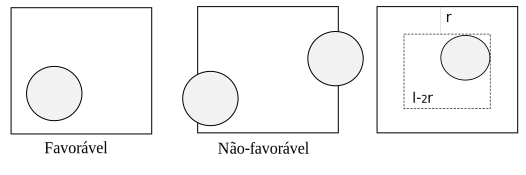
\includegraphics[angle=0, scale=0.5]{fig7.pdf}
\end{center}
\caption{\label{fig7} Representação esquemática do jogo dos ladrilhos.
}
\end{figure} 
  Portanto, a probabilidade da moeda cair inteiramente
dentro de um ladrilho é $$ \frac{( l-2r )^2}{l^2}.$$
Se consideramos um piso formado por quadrados de cerâmica de 30 cm de lado e um disco (``moeda'') de raio 5 cm, a probabilidade do disco cair inteiramente dentro de um dos ladrilhos é igual a $(30-10)^2/ 30^2 = 0,4444$ ou 44,44\%.


Nessa situação, o diâmetro $d$ do disco que daria 60\% de chances de vitória ao jogador é $d$ = 6,77 cm.
\end{frame}
%=====================================================================



\begin{frame}
\frametitle{\textbf{Exercícios}}
\baselineskip=13pt
\begin{block}{}
	
	
	
	\begin{example}
		Se $A$, $B$ e $C$ forem eventos mutuamente excludentes, com $P(A)=0{,}2$, $P(B)=0{,}3$ e $P(C)=0{,}4$, determine:
		\begin{enumerate}
			\item[(a)] $P(A\inter B\inter C)$.
			\item[(b)] $P(A^c\union(B\union C))$.
			\item[(c)] $P((A\union B)\inter C)$.
		\end{enumerate}
		
	\end{example}
	
	\begin{example}
		Se $A$, $B$ e $C$ forem eventos mutuamente excludentes, será possível obter $P(A)=0{,}3$, $P(B)=0{,}4$ e $P(C)=0{,}5$? Justifique.
	\end{example}
	
\end{block}
\end{frame}


\begin{frame}
\frametitle{\textbf{Exercícios}}
\baselineskip=13pt
%\begin{block}{}

\begin{example}
Se $\Omega=\{a,b,c\}$, e a álgebra $\A$ é o conjunto das partes de
$\Omega$, e a medida de probabilidade $P$ é parcialmente definida
por
$$P(\{a,b\})=0.5\mbox{,  }P(\{b,c\})=0.8\mbox{,  }P(\{a,c\})=0.7,$$
então complete a especificação de $P$ para todos os eventos em $\A$.
\end{example}

\begin{example}
Se $\{A_i\}$ for uma partição enumerável de $\Omega$ e
$P(A_i)=ab^i$, $i\geq 1$, então quais as condições que $a$ e $b$
devem satisfazer para que $P$ seja uma medida de probabilidade?
\end{example}

%\end{block}
\end{frame}

\begin{frame}
\frametitle{\textbf{Exercícios}}
\baselineskip=13pt
%\begin{block}{}


\begin{example}
Em um grupo de $r$ pessoas qual a probabilidade de haver pelo menos
duas pessoas que façam aniversário no mesmo dia, assumindo que a
distribuição de aniversários é uniforme ao longo do ano e
desprezando a existência de anos bissextos?
\end{example}

\end{frame}

\begin{frame}
\frametitle{\textbf{Solução}}
\baselineskip=13pt


O número de resultados possíveis para os
aniversários de $r$ pessoas é $365^r$. O número de casos possíveis
onde todas as pessoas fazem aniversário em dias diferentes é dado
por $365\times 364\times \cdots\times(365-(r-1))$. Portanto, o
número de casos possíveis onde pelo menos duas pessoas fazem
aniversário no mesmo dia é a diferença entre o número total de
aniversários possíveis e o número de casos onde as pessoas têm
aniversários em datas diferentes, ou seja, é igual a
$$365^r-365\times 364\times \cdots\times(365-(r-1)).$$
Logo, a probabilidade deste evento é:
$$1-\frac{365\times 364\times \cdots\times(365-(r-1))}{365^r}.$$
Para $r=23$, temos que essa probabilidade é aproximadamente igual a
$0,51$. E para $r=50$, essa probabilidade é igual a $0,97$.

%\end{block}
\end{frame}

\begin{frame}
\frametitle{\textbf{Exercícios}}
\baselineskip=13pt
%\begin{block}{}


\begin{example}
Em uma loteria de $N$ números há um só prêmio. Salvador compra $n$
$(1<n<N)$ bilhetes para uma só extração e Sílvio compra $n$
bilhetes, um para cada uma de $n$ extrações. Qual dos dois jogadores
têm mais chances de ganhar algum prêmio?
\end{example}
\end{frame}

\begin{frame}
\frametitle{\textbf{Solução}}
\baselineskip=13pt

A probabilidade de Salvador ganhar algum prêmio é
$\frac{n}{N}$. O número total de $n$ extrações possíveis é $N^n$. O
número de casos onde Sílvio não ganha nenhum prêmio é $(N-1)^n$,
logo o número de casos onde Sílvio ganha algum prêmio é igual a
$N^n-(N-1)^n$. Logo, a probabilidade de Sílvio ganhar algum prêmio é
$1-\frac{(N-1)^n}{N^n}$.

Vamos provar por indução que Salvador tem mais chance de ganhar, ou
seja, $\frac{n}{N}>1-\frac{(N-1)^n}{N^n}$, que equivale a
$$\frac{(N-1)^n}{N^n}>1-\frac{n}{N}.$$
Para $n=2$, temos:
$$\frac{(N-1)^2}{N^2}=1-\frac{2}{N}+\frac{1}{N^2}>1-\frac{2}{N}.$$
\end{frame}

\begin{frame}
\frametitle{\textbf{Solução (cont.)}}
\baselineskip=13pt

Suponha que para $n=k$, temos que
$$\frac{(N-1)^k}{N^k}>1-\frac{k}{N}.$$
Multiplicando esta expressão por $\frac{N-1}{N}$, obtemos:
\begin{eqnarray}
& & \frac{(N-1)^{k+1}}{N^{k+1}}>(\frac{N-1}{N})(1-\frac{k}{N})\nonumber\\
& & =1-\frac{1}{N}-\frac{k}{N}+\frac{k}{N^2}>1-\frac{k+1}{N}.\nonumber
\end{eqnarray}

%\end{block}
\end{frame}

\begin{frame}
\frametitle{\textbf{Exercícios}}
\baselineskip=13pt
%\begin{block}{}


\begin{example}
Doze pessoas são divididas em três grupos de 4. Qual é a
probabilidade de duas determinadas dessas pessoas ficarem no mesmo
grupo?
\end{example}
\end{frame}


\begin{frame}
\frametitle{\textbf{Solução}}
\baselineskip=13pt

O número total de divisões de doze pessoas em 3
grupos de 4 é igual a $\binom{12}{4}\binom{8}{4}\binom{4}{4}$. Vamos
agora contar o número de casos favoráveis ao nosso evento. Existem 3
opções de escolhermos em qual grupo as duas pessoas determinadas
podem ficar. Das 10 pessoas restantes, temos que escolher mais duas
para estarem neste grupo, o que podemos fazer de $\binom{10}{2}$
maneiras diferentes. E temos $\binom{8}{4}\binom{4}{4}$ maneiras
diferentes de dividir as outras 8 pessoas nos dois grupos restantes.
Portanto, a probabilidade de duas determinadas pessoas ficarem no
mesmo grupo é:
$$\frac{3\binom{10}{2}\binom{8}{4}\binom{4}{4}}{\binom{12}{4}\binom{8}{4}\binom{4}{4}}=\frac{3}{11}.$$

%\end{block}
\end{frame}

\begin{frame}
\frametitle{\textbf{Exercícios}}
\baselineskip=13pt
%\begin{block}{}


\begin{example}
Suponha que temos em uma sala $n$ mães cada uma com um filho. Suponha formemos duplas aleatoriamente, onde cada dupla contém uma mãe e um filho, qual a probabilidade de que pelo menos uma mãe forme uma dupla com seu próprio filho?
\end{example}

\end{frame}

\begin{frame}
\frametitle{\textbf{Solução}}
\baselineskip=13pt

Seja $A_i$ o evento que a $i$-ésima mãe forma dupla com seu filho. Queremos determinar
$$P(\cup_{i=1}^{n}A_i).$$
Vamos calcular esta probabilidade utilizando a fórmula da inclusão exclusão. Note que:
\begin{eqnarray}
& & P(A_i)=\frac{(n-1)!}{n!}=\frac{1}{n}\mbox{ para todo } i\in\{1,2,\ldots,n\} \nonumber\\
& & P(A_i\cap A_j)=\frac{(n-2)!}{n!}=\frac{1}{n(n-1)}\mbox{ para }i\ne j \nonumber
\end{eqnarray}
e em geral, para um grupo $I\in\{1,2,\ldots,n\}$ de mães temos que
$$P(\cap_{i\in I}A_i)=\frac{(n-||I||)!}{n!}.$$

\end{frame}

\begin{frame}
\frametitle{\textbf{Solução (cont.)}}
\baselineskip=13pt

Como existem $\binom{n}{||I||}$ grupos de mães com cardinalidade $||I||$, temos que
\begin{eqnarray}
& & P(\cup_{i=1}^{n}A_i)=\sum_{i=1}^{n}(-1)^{i+1}\binom{n}{i}\frac{(n-i)!}{n!} \nonumber\\
& & = \sum_{i=1}^{n}(-1)^{i+1}\frac{1}{i!}\nonumber
\end{eqnarray}
Note que quando $n\rightarrow\infty$, temos que esta probabilidade tende a $1-\frac{1}{e}$.


%\end{block}
\end{frame}

\begin{frame}
\frametitle{\textbf{Exercícios}}
\baselineskip=13pt
%\begin{block}{}


\begin{example}
Demonstre que se $P(A_i)=1$ para $i=1,2,\ldots$, então $P(\cap_{i=1}^{\infty}A_i)=1$.

{\bf Solução: } Como $P(A_i)=1$, temos que $P(A_i^c)=1-P(A_i)=0$. Logo pela não-negatividade e pela desigualdade de Boole, temos
$0\leq P(\cup_{i=1}^{\infty}A_i^c)\leq \sum_{i=1}^{\infty}P(A_i^c)=0$. Portanto, como pela Lei de De'Morgan, $\cap_{i=1}^{\infty}A_i=(\cup_{i=1}^{\infty}A_i^c)^c$, temos que
$P(\cap_{i=1}^{\infty}A_i)=1-P(\cup_{i=1}^{\infty}A_i^c)=1$.
\end{example}

\end{frame}

\begin{frame}
\frametitle{\textbf{Exercícios}}
\baselineskip=13pt

\begin{example}
Demonstre: se $A_1,A_2,\ldots$ e $B_1,B_2,\ldots$ são eventos aleatórios do mesmo espaço de probabilidade tais que
$P(A_n)\rightarrow 1$ e $P(B_n)\rightarrow p$, então $P(A_n\cap B_n)\rightarrow p$.

{\bf Solução: } Note que
\begin{eqnarray}
& & P(A_n\cap B_n)=1-P((A_n\cap B_n)^c)=1-P(A_n^c\cup B_n^c) \nonumber \\
& & \geq 1-P(A_n^c)-P(B_n^c)=P(A_n)+P(B_n)-1.
\end{eqnarray}
Como $P(A_n)+P(B_n)-1\rightarrow p$, temos que $\liminf P(A_n\cap B_n)\geq p$. Por outro lado, como $P(A_n\cap B_n)\leq P(B_n)$ e $P(B_n)\rightarrow p$, temos que $\limsup P(A_n\cap B_n)\leq p$. Portanto, $\lim P(A_n\cap B_n)=p$.
\end{example}

%\end{block}
\end{frame}


% % 
% % %=====================================================================
% % \begin{frame}
% %  
% % \end{frame}
% % %=====================================================================
% % 
% % %=====================================================================
% % \begin{frame}
% %  
% % \end{frame}
% % %=====================================================================
% % 
% % 
% % %=====================================================================
% % \begin{frame}
% %  
% % \end{frame}
% % %=====================================================================
% % 
% % 
% % %=====================================================================
% % \begin{frame}
% %  
% % \end{frame}
% % %=====================================================================
% % 
% % %=====================================================================
% % \begin{frame}
% %  
% % \end{frame}
% % %=====================================================================
% % 
% % %=====================================================================
% % \begin{frame}
% %  
% % \end{frame}
% % %=====================================================================
% % 
% % %=====================================================================
% % \begin{frame}
% %  
% % \end{frame}
% % %=====================================================================
% % 
% % 
% % %=====================================================================
% % \begin{frame}
% %  
% % \end{frame}
% % %=====================================================================
% % 
% % 
% % %=====================================================================
% % \begin{frame}
% %  
% % \end{frame}
% % %=====================================================================
% % 
% % %=====================================================================
% % \begin{frame}
% %  
% % \end{frame}
% % %=====================================================================
\end{document}

